\DocumentMetadata{
  pdfversion=2.0,
  lang=es-MX,
  pdfstandard=ua-2
}

\documentclass{sener2025}

\addbibresource{referencias.bib}

% --- Metadatos PDF/UA (Accesibilidad Universal) ---
\hypersetup{
  pdftitle={Plan de Desarrollo del Sector Hidrocarburos},
  pdfauthor={SENER},
  pdfsubject={PLADESHI 2025},
  pdfkeywords={Energía},
  pdfcreationdate={D:20260130185400},
  pdfversion={1}
}

% --- Metadatos del Documento ---
\title{Plan de Desarrollo del Sector Hidrocarburos}
\subtitle{PLADESHI 2025}
\author{SENER}
\date{27/1/2026}
\institucion{Secretaría de Energía (SENER)}
\unidad{Subsecretaria de Planeación y Transición Energética}
\setDocumentoCorto{PLADESHI 2025}
\palabrasclave{Energía}
\version{1}

\begin{document}

\portadafondo[img/PLADESHIportada.jpg]

\tableofcontents
\newpage

\listafiguras
\newpage

\listatablas
\newpage

\clearpage
\begin{center}
{\Large\patriafont\bfseries\color{gobmxGuinda}Presentación}\\[1cm]
\end{center}

El sector de hidrocarburos constituye un componente fundamental del sistema energético nacional y un elemento esencial para la seguridad, la soberanía y la estabilidad económica del país. Su desarrollo ordenado y sustentable resulta indispensable para asegurar el abastecimiento energético, fortalecer la industria nacional y garantizar la continuidad de las actividades productivas que sustentan el bienestar de la población.

En congruencia con los objetivos establecidos en el Plan Nacional de Desarrollo 2025–2030 (PND 2025–2030), el Gobierno de México impulsa una política energética integral que promueve el aprovechamiento eficiente y responsable que contribuye al fortalecimiento de la soberanía energética de la Nación.

El Plan de Desarrollo del Sector de Hidrocarburos (en adelante, PLADESHi) es el instrumento de planeación de largo plazo previsto en la Ley de Planeación y Transición Energética publicada en el Diario Oficial de la Federación el 18 de marzo de 2025 (en adelante, LPTE), mediante el cual se orienta la expansión y modernización de la infraestructura del sector. Su propósito es prever y coordinar las acciones necesarias para garantizar el suministro oportuno, suficiente y sostenible de hidrocarburos y sus derivados, con un horizonte de planeación de quince años y revisiones anuales que permitan su adecuación a la evolución tecnológica, económica y ambiental del país.

La elaboración del PLADESHi reconoce que los hidrocarburos continúan desempeñando un papel relevante en la matriz energética nacional durante el proceso de transición hacia el aprovechamiento de fuentes de energía más limpias y sostenibles. En este sentido, se establecen las directrices para optimizar la utilización de los recursos nacionales, incrementar la eficiencia de las operaciones, reducir las emisiones asociadas y fortalecer la seguridad energética bajo criterios de responsabilidad ambiental y social.

Así, el PLADESHi articula, en un marco único de planeación, las acciones estratégicas de exploración, extracción, procesamiento, refinación, formulación, tratamiento, transporte, almacenamiento, distribución, expendio, comercialización de hidrocarburos, importación, exportación, así como la modernización de la infraestructura, el fortalecimiento tecnológico y la integración de cadenas de valor que impulsen la competitividad nacional. Conforme a lo establecido en la LPTE, la Secretaría de Energía (en adelante, SENER) conduce su elaboración y actualización, con la participación de las entidades y empresas públicas del Estado, particularmente Petróleos Mexicanos (en adelante, PEMEX) y sus empresas filiales, en coordinación con otros participantes del sector.

El PLADESHi se alinea con el PND 2025-2030, principalmente en lo correspondiente al Eje 4 Desarrollo Sustentable, y contribuye a los ejes transversales: 2 Innovación pública para el desarrollo tecnológico nacional y 3 Derechos de los pueblos y las comunidades indígenas y agromexicanas. Esta alineación se realiza en cumplimiento del artículo 21, fracción V de la Ley de Planeación y Transición Energética (LPTE), la cual es reglamentaria de los artículos 25 (párrafo tercero), 27 (párrafos sexto y séptimo) y 28 (párrafo cuarto) de la Constitución Política de los Estados Unidos Mexicanos. Asimismo, en concordancia con el artículo 8 de la Ley del Sector Hidrocarburos, el PLADESHi considera los siguientes principios rectores:

\begin{itemize}
  \item Soberanía y seguridad energética, mediante el fortalecimiento de la producción nacional, la confiabilidad del suministro y la reducción de la dependencia externa.
  \item Eficiencia y modernización del sector, promoviendo la innovación tecnológica, la mejora continua de los procesos y la reducción de pérdidas.
  \item Transición energética ordenada y sustentable, que impulse la descarbonización progresiva y el aprovechamiento más limpio de los hidrocarburos.
  \item Desarrollo productivo y regional, orientado a generar valor agregado nacional, empleo digno y encadenamientos industriales estratégicos.
  \item Transparencia, rendición de cuentas y gobernanza institucional, que consoliden la legitimidad de las decisiones públicas y la participación informada de la sociedad.
\end{itemize}
El PLADESHi representa un instrumento de Estado que orienta la política pública y las inversiones estratégicas en el país en materia de hidrocarburos. Constituye, al mismo tiempo, una expresión del compromiso del Gobierno de México con la seguridad energética, la soberanía nacional y la transición hacia un sistema energético con infraestructura moderna, eficiente y sostenible, en beneficio del pueblo de México.



\portadaseccion{1}{Introducción}{}

\section{Introducción}




\subsection{Marco jurídico}

Los artículos 25, 27 y 28 de la Constitución Política de los Estados Unidos Mexicanos establecen los principios y mandatos rectores, así como la base del marco jurídico para la planeación en el sector hidrocarburos, al definir la propiedad de la Nación y el control del Estado sobre estos recursos estratégicos.

El artículo 25 constitucional confiere al Estado la rectoría del desarrollo nacional, lo que implica la responsabilidad de planear, conducir y orientar la actividad económica de manera integral y sustentable, que fortalezca la soberanía de la Nación. Dentro de este mandato constitucional, se precisa que el Estado planeará, conducirá, coordinará y orientará la actividad económica nacional, y llevará a cabo la regulación y fomento de las actividades que demande el interés general.

Bajo esta tesitura, el sector hidrocarburos se define como un área estratégica que está a cargo del Estado y que debe ser impulsada y organizada por éste, en concurrencia con los sectores público y privado, siempre con el objetivo de fortalecer la soberanía de la Nación y el bienestar social.

De forma complementaria, el artículo 27 de la Constitución establece la propiedad de la Nación sobre los yacimientos de petróleo y demás hidrocarburos, señalando su naturaleza jurídica imprescriptible e inalienable. En consecuencia, el Estado tiene la atribución exclusiva para realizar las actividades de exploración y extracción, mediante empresas públicas del Estado o a través de contratos con particulares.

Por otro lado, el artículo 28 constitucional mandata la prohibición de los monopolios y las prácticas monopólicas en los Estados Unidos Mexicanos, a fin de promover la competencia económica como un principio general. No obstante, el mismo precepto contempla una excepción a dicho principio y establece que no constituirán monopolios las funciones que el Estado ejerza en diversas áreas estratégicas, entre las cuales, se encuentra el sector energético, particularmente, las relativas a la exploración y extracción del petróleo y de los demás hidrocarburos. Esto con el objetivo de preservar la seguridad y autosuficiencia energética de la Nación, evitando el lucro, así como garantizar la seguridad nacional y soberanía a través de la Empresa Pública del Estado que se establezca para tal efecto. Esta disposición, mantiene al Estado como el agente rector y planificador que asegura el control estratégico del sector.

En resumen, este conjunto de mandatos constitucionales previstos para el sector fortalece las condiciones y capacidades del Estado en las actividades de exploración y extracción del petróleo y de los demás hidrocarburos, además, ordena e incentiva la participación de los privados a través de la implementación de diversos esquemas, bajo la premisa de que dicha participación no puede ser mayor a la del Estado.

De igual forma, la Ley Orgánica de la Administración Pública Federal, señala en su artículo 33, fracciones I, II, IV, V y XXV que, corresponde a la SENER, entre otras atribuciones: establecer, conducir y coordinar la política energética del país; ejercer los derechos de la Nación mediante la exploración y extracción del petróleo y de los demás hidrocarburos; promover la participación de los particulares en las actividades del sector; llevar a cabo la planeación vinculante en el sector energético, que atienda la preservación de la soberanía y seguridad energéticas, el mejoramiento de la productividad energética, la restitución de reservas de hidrocarburos, la diversificación de las fuentes de combustibles, la reducción progresiva de impactos ambientales de la producción y consumo de energía, la mayor participación de las energías renovables en el balance energético nacional, la satisfacción de las necesidades energéticas básicas de la población, el ahorro de energía y la mayor eficiencia de su producción y uso, el fortalecimiento de las Empresas Públicas del Estado del sector energético, entre otras; así como procurar, fomentar y vigilar el adecuado suministro de los combustibles en el territorio nacional.

Asimismo, la LPTE, establece en su artículo 2 que la SENER está a cargo de la planeación vinculante en el Sector Energético, que incluye el desarrollo de las áreas estratégicas para preservar la soberanía, la seguridad, la autosuficiencia y la Justicia Energética de la Nación. En particular, para el sector hidrocarburos, la LPTE dispone en sus artículos 3, fracción XIX, 8, fracción I, 21, fracción V, y 31, primer párrafo, que corresponde a la SENER elaborar y publicar, entre otros instrumentos, el Plan de Desarrollo del Sector Hidrocarburos (en adelante PLADESHi), así como coordinar su ejecución y vigilar su cumplimiento.

Así, el PLADESHi es el instrumento rector de planeación para el desarrollo y modernización de la infraestructura del sector hidrocarburos a nivel nacional. De conformidad con el artículo 31 de la LPTE, el PLADESHi es de carácter vinculante y se constituye como el documento de desarrollo y modernización de la infraestructura del sector hidrocarburos con un horizonte de quince años, que debe ser congruente con la Estrategia Nacional de Transición Energética, el PND 2025–2030, el Programa Sectorial de Energía y el Plan para la Transición Energética y el Aprovechamiento Sustentable de la Energía.

En consonancia con lo anterior, la Ley del Sector Hidrocarburos establece, en su artículo 7, que la regulación de las actividades del sector hidrocarburos debe sujetarse y contribuir a los objetivos y acciones determinados en el PND y la política pública que determine la persona Titular del Ejecutivo Federal, a través de la SENER. Además, el artículo 8 de la mencionada Ley señala que la planeación del sector hidrocarburos tiene carácter vinculante, misma que debe promover la justicia energética, la transición y eficiencia energéticas, la sustentabilidad y el desarrollo de energías limpias y renovables; preservar la soberanía y seguridad energética, así como proveer al pueblo combustibles de la mejor calidad y al menor precio posible; e incentivar el desarrollo, modernización de la infraestructura del sector, tomando en cuenta la seguridad, eficiencia y sustentabilidad operativa de este.

De esta forma, el carácter vinculante de la planeación del sector hidrocarburos se reitera con lo establecido en el artículo 336 del Reglamento de la Ley del Sector Hidrocarburos, el cual señala que las actividades reguladas deben realizarse con base en criterios de eficiencia, eficacia, mejores prácticas, sustentabilidad y seguridad operativa, a fin de contribuir a la justicia energética, conforme los instrumentos en materia de planeación y transición energética.

Finalmente, el PLADESHi se alinea con los Cien Compromisos para el Segundo Piso de la Cuarta Transformación, apartado X. “República soberana y con energía sustentable” y con el Eje General 4. “Desarrollo Sustentable” del PND 2025–2030, el cual establece como objetivo recuperar la rectoría del sector energético, lo que implica fortalecer a las Empresas Públicas del Estado, que en materia de hidrocarburos es PEMEX, a través de inversión, eficiencia, sustentabilidad, austeridad y combate a la corrupción, asegurando su solidez financiera.

En línea con el PND y el Programa Sectorial de Energía 2025-2030, el PLADESHi contempla el desarrollo de petroquímica nacional y la producción de fertilizantes, lo que es congruente con el principio de soberanía alimentaria y los criterios de planeación de “máximo beneficio colectivo, aprovechamiento inteligente del patrimonio energético, cohesión social, equilibrios regionales. Además, enfatiza la necesidad de reducir emisiones de efecto invernadero y adoptar tecnologías limpias para avanzar hacia la descarbonización en el sector hidrocarburos.

De esta manera, el PLADESHi no sólo cumple un mandato jurídico, sino que constituye una herramienta estratégica para consolidar la seguridad del abastecimiento nacional de hidrocarburos, reducir la dependencia de importaciones críticas, modernizar la infraestructura del sector e impulsar un aprovechamiento responsable de estos recursos en el marco de la transición energética.

La Secretaría de Energía, en el ámbito de sus atribuciones emitirá las disposiciones administrativas que establezcan los criterios de planeación vinculante aplicables al otorgamiento de permisos, a efecto de asegurar que los proyectos sean congruentes con los objetivos, prioridades y metas del presente plan, así como a los demás Instrumentos de Planeación del Sector Energético.


\subsection{Alcances}

El PLADESHi considera los "Cien Compromisos para el Segundo Piso de la Cuarta Transformación", específicamente los compromisos incluidos en el apartado República Soberana y con Energía Sustentable que son los siguientes:

\begin{itemize}
  \item Fortalecimiento de PEMEX y la Comisión Federal de Electricidad (CFE) como empresas públicas del Estado.
  \item La producción de PEMEX priorizará el consumo nacional.
  \item Fuerte impulso a la eficiencia y racionalidad energéticas.
  \item Aumento de producción nacional de petroquímicos y fertilizantes.
\end{itemize}
De igual forma, se alinea con el Eje General 4 Desarrollo sustentable, del PND:

\begin{itemize}
  \item Mantener e incrementar la producción de hidrocarburos para reducir la dependencia externa y asegurar el abastecimiento energético.
  \item Ampliar las reservas de hidrocarburos de forma sustentable mediante proyectos estratégicos de exploración y producción.
  \item Fortalecer las capacidades operativas y financieras de las empresas públicas del Estado, priorizando la eficiencia y el desempeño ambiental.
  \item Consolidar la producción de biofertilizantes en la petroquímica de PEMEX para fortalecer la producción agroecológica y el desarrollo sustentable en comunidades con mayor rezago.
\end{itemize}
Conforme al PND se consideran también las siguientes Estrategias:

\begin{itemize}
  \item 4.2.1 Fomentar la transición gradual de combustibles fósiles a energías renovables para fortalecer la sustentabilidad económica y ambiental.
  \item 4.2.3 Fomentar el aprovechamiento eficiente y sustentable de los recursos energéticos para fortalecer la seguridad energética y reducir el impacto ambiental.
  \item 4.2.4 Promover la integración de energías limpias y renovables en todas las etapas de las cadenas de valor para garantizar un suministro energético sustentable y competitivo.
  \item 4.3.1. Reducir las emisiones de gases de efecto invernadero para mitigar el cambio climático y sus impactos en la sociedad, la economía y el medio ambiente.
  \item 4.3.2. Implementar políticas de mitigación y adaptación al cambio climático con enfoque en derechos humanos, igualdad y justicia ambiental para fortalecer la resiliencia de la sociedad y los ecosistemas.
  \item 4.4.1. Desarrollar esquemas que amplíen el acceso a la energía en comunidades y regiones con pobreza energética, garantizando un suministro confiable, asequible y sustentable.
  \item 4.4.2 Garantizar el suministro de electricidad y combustibles a toda la población mediante mecanismos de ajuste de precios que aseguren su asequibilidad y estabilidad.
  \item 4.4.3 Facilitar trámites y procesos administrativos para comunidades rurales e industrias con infraestructura de autoabastecimiento energético, asegurando un acceso eficiente y sustentable a la energía.
\end{itemize}
En congruencia con la política energética nacional, el presente Plan incorpora las directrices y medidas anunciadas por la persona Titular del Ejecutivo Federal, la Doctora Claudia Sheinbaum Pardo, tales como:

\begin{itemize}
  \item Plan Nacional de Desarrollo 2025–2030.
  \item Plan México.
  \item Plan de Trabajo 2025-2030 de Petróleos Mexicanos.
  \item Plan Estratégico 2025- 2035 de Petróleos Mexicanos.
  \item Plan de Sustentabilidad de Petróleos Mexicanos.
\end{itemize}
Para la elaboración del PLADESHi, la SENER también considera las siguientes definiciones:

\begin{itemize}
  \item Exploración eficiente: optimizar los procesos para identificar nuevas reservas de petróleo y gas.
  \item Producción sustentable: implementar prácticas responsables con el medio ambiente para asegurar una producción sostenible.
  \item Refinación reforzada: mejorar la capacidad y eficiencia de las refinerías existentes y construir nuevas infraestructuras.
  \item Producción de petroquímicos y fertilizantes: aumentar la producción de estos productos esenciales.
  \item Logística segura y eficiente: modernizar los sistemas de transporte y distribución para garantizar un suministro continuo y seguro.
  \item Generación de energía limpia: integrar fuentes de energía renovable para diversificar la matriz energética del país.
  \item Eficiencia Energética: Todas las acciones que conlleven a una reducción, económicamente viable, de la cantidad de energía que se requiere para satisfacer las necesidades energéticas de los servicios y bienes que demanda la sociedad, asegurando un nivel de servicio igual o superior.
  \item Cogeneración: Generación de energía eléctrica producida de manera conjunta con vapor u otro tipo de energía térmica secundaria útil o ambos; producción directa o indirecta de energía eléctrica mediante la energía térmica no aprovechada en los procesos, o generación directa o indirecta de energía eléctrica cuando se utilicen combustibles producidos en los procesos industriales.
  \item Cogeneración Eficiente: La energía generada por centrales de Cogeneración, en términos de los criterios generales emitidos por la Secretaría, los criterios técnicos y metodologías emitidos por la Comisión Nacional de Energía y las metodologías de Emisiones establecidas por la Secretaría de Medio Ambiente y Recursos Naturales.
\end{itemize}
En este sentido, el PLADESHi concentra en un solo marco de planeación los instrumentos estratégicos del sector hidrocarburos, incluyendo los programas de desarrollo de infraestructura, de modernización de instalaciones y de fortalecimiento operativo de las empresas públicas del Estado.


\subsection{Acuerdos de cooperación internacional}

El PLADESHi se encuentra alineado con los compromisos internacionales asumidos por el Estado Mexicano en materia de desarrollo sostenible, energía, cambio climático, derechos humanos y cooperación económica. Estos compromisos orientan la planeación, ejecución y seguimiento de las políticas públicas del sector hidrocarburos, en congruencia con la Constitución Política de los Estados Unidos Mexicanos y el PND 2025–2030.

México es parte de la Carta de las Naciones Unidas y de la Agenda 2030 para el Desarrollo Sostenible, por lo que está comprometido con el cumplimiento de los Objetivos de Desarrollo Sostenible (ODS). Los ODS que se buscan impulsar en el sector hidrocarburos son principalmente el ODS 7 “Energía asequible y no contaminante”, el ODS 9 “Industria, innovación e infraestructura”, el ODS 12 “Producción y consumo responsables” y el ODS 13 “Acción por el clima”, los cuales orientan la transición hacia un sector energético más limpio, seguro y eficiente.

Asimismo, el Estado Mexicano es parte del Acuerdo de París, adoptado en el marco de la Convención Marco de las Naciones Unidas sobre el Cambio Climático (CMNUCC), instrumento que establece Contribuciones Determinadas a Nivel Nacional (NDC, por sus siglas en inglés) para reducir emisiones de gases de efecto invernadero (GEI) y promover la transición energética. En cumplimiento de dicho acuerdo, el PLADESHi incorpora estrategias orientadas a la descarbonización progresiva del sector, al uso de tecnologías de bajo impacto ambiental y a la eficiencia energética en toda la cadena de valor de los hidrocarburos.

En materia de cooperación económica y energética, México forma parte de la Organización para la Cooperación y el Desarrollo Económicos (OCDE) y del Tratado entre México, Estados Unidos y Canadá (T-MEC). Este último establece disposiciones sobre la transparencia regulatoria, la protección del medio ambiente y el fomento de prácticas responsables en el sector energético, sin menoscabo de la soberanía energética nacional sobre los recursos naturales, reconocida expresamente en su Capítulo 8.

De igual forma, México participa en organismos internacionales especializados como la Agencia Internacional de Energía (AIE) y la Organización Latinoamericana de Energía (OLADE), los cuales promueven la cooperación técnica y el intercambio de mejores prácticas en materia de planeación, seguridad energética, diversificación de fuentes y desarrollo sostenible. Estas instancias constituyen referentes técnicos para la elaboración y actualización del PLADESHi.

En el contexto regional, México ha suscrito la Declaración de Lima sobre Seguridad Energética y Transición Justa en América Latina y el Caribe, así como acuerdos de cooperación con países de la región para promover la innovación tecnológica, la eficiencia energética y el aprovechamiento sostenible de los recursos fósiles y renovables.

En conjunto, estos instrumentos internacionales constituyen el marco jurídico y de cooperación global que orienta el diseño y ejecución del PLADESHi. Con ello se garantiza que la política de desarrollo del sector hidrocarburos se lleve a cabo conforme a los principios de sustentabilidad, soberanía energética, seguridad energética, equidad intergeneracional y responsabilidad ambiental.


\subsection{Evaluación de los impactos sociales de los proyectos del sector hidrocarburos}

El PLADESHi busca que el desarrollo y modernización de la infraestructura del sector hidrocarburos incorpore no solo un enfoque de planeación vinculante, sino también un enfoque de justicia energética y social. Bajo esta premisa, la Manifestación de Impacto Social en el Sector Energético (MISSE) y sus planes de gestión social buscan garantizar que cada nuevo proyecto del sector se traduzca en bienestar tangible para las comunidades.

La MISSE analiza los efectos positivos y negativos que resultan del desarrollo de un proyecto y propone un plan de gestión social que amplifique impactos positivos, prevenga y mitigue impactos negativos, que permitan promover la justicia energética, así como el respeto a los derechos humanos y la sustentabilidad. Si bien la anterior Evaluación de Impacto Social (EvIS) incorporó la gestión social como un aspecto a considerar en el desarrollo de proyectos energéticos, no era vinculante ni existía la posibilidad de verificación. En cambio, la MISSE, bajo el nuevo marco legal, establece obligaciones claras de reporte y seguimiento, habilita la verificación y consolida una mayor participación efectiva de las comunidades. Con ello, se brinda certeza a todas las partes y se asegura que los beneficios lleguen a quienes más lo necesitan.

Los planes de gestión social y sus estrategias de inversión se orientan actualmente a reducir la pobreza energética, atender a las poblaciones más vulnerables, y fortalecer cadenas productivas y capacidades locales; mediante un enfoque participativo que responda a las necesidades reales de la comunidad. En este sentido, se busca detonar una inversión social relevante que beneficie directamente a las comunidades y promueva oportunidades económicas que impulsen el desarrollo y la prosperidad compartida.

Asimismo, los pueblos y comunidades indígenas y afromexicanas adquieren un papel central en la construcción de un sector energético más justo. Los procesos de consulta previa, libre e informada garantizan que sus necesidades sean consideradas y que exista una participación equitativa en los beneficios derivados de los proyectos que se desarrollan en sus territorios. En síntesis, la evaluación de los impactos sociales, acompañadas de estrategias de inversión social relevantes y orientadas a atender las necesidades locales, forma parte de una planeación ordenada, con sentido social y de justicia energética en el sector hidrocarburos.


\subsection{Justicia Social}

El PLADESHi retoma el concepto de Justicia Energética (SENER, 2025, 67), que es un principio fundamental y eje rector del nuevo modelo energético en México. Desde esta perspectiva, la energía no se concibe como una mercancía, sino como un derecho que garantiza la dignidad y el bienestar compartido. Su objetivo principal es asegurar un acceso equitativo, asequible y seguro a la energía, de modo que esta contribuya de manera directa al bienestar de la población. La política de justicia energética busca proteger la economía familiar, reducir la brecha de las desigualdades históricas y consolidará la energía en un factor de cohesión social. Asimismo, este principio se ha incorporado al marco legal del sector energético para orientar la asignación de recursos que permitan reducir la pobreza energética de los hogares.

En este contexto, la SENER articula la política de justicia energética en el sector hidrocarburos a través de las siguientes líneas de acción:


\subsubsection{Estrategia para Estabilizar los Precios de la Gasolina y GLP}

La estabilización de los precios de las gasolinas y del Gas Licuado de Petróleo (GLP) es una medida clave para proteger el bienestar de las familias y reducir la vulnerabilidad económica, especialmente de los hogares con menores ingresos. Al evitar aumentos abruptos, se promueve la justicia energética, entendida como el acceso equitativo y asequible a la energía, garantizando que todas las personas puedan cubrir sus necesidades básicas sin que el costo de los energéticos se convierta en una carga desproporcionada o en un factor de exclusión social.

A partir de marzo de 2025, se implementó una estrategia para mantener el precio de la gasolina regular por debajo de los 24 pesos por litro en más de 12,400 estaciones de servicio a nivel nacional. Esta medida fue clave para que la inflación se ubicara en 3.51\% en julio de 2025, protegiendo la economía de los hogares. En el nuevo modelo energético, la visión al 2030 es garantizar el acceso universal a la energía, especialmente en comunidades rurales y marginadas, manteniendo la política de no aumentar precios y tarifas por encima de la inflación (SENER, 2025, 67-70).

Con la creación de Gas Bienestar, en agosto de 2021, el Gobierno de México cumple el compromiso de que los energéticos no se incrementen por encima de la inflación y cumple con el propósito de vender el energético a un precio justo para todos, particularmente en zonas urbanas de alta demanda y menor poder adquisitivo. Desde su creación, junto con el restablecimiento del esquema regulado de precios máximos del GLP, ha contribuido a proteger la economía familiar frente a los incrementos de este energético, garantizar su estabilidad y establecerse como un referente en el precio y calidad en el mercado interno.

Entre octubre de 2024 y agosto de 2025, el precio al público del GLP se mantuvo estable, registrando un incremento de apenas 0.96 pesos por kilogramo, lo que representa un aumento de solo 5\% a pesar de la alta volatilidad en el mercado global. El éxito del programa se refleja en su contribución a la estabilidad de precios, la competencia justa y el bienestar para las familias mexicanas.

Para evitar aumentos desproporcionados, la SENER implementó mesas de trabajo permanentes con los distribuidores de GLP para monitorear los costos operativos y establecer mecanismos que aseguren precios justos, confiables y accesibles para la población. A finales de agosto de 2025, se alcanzó un acuerdo equilibrado con los empresarios del sector para mantener los precios accesibles y asegurar que no superen los incrementos de la inflación, reafirmando el compromiso del Gobierno de México con la justicia social y energética.


\subsubsection{Sistema de Gasolineras del Bienestar}

Las Gasolineras del Bienestar son un proyecto del Gobierno mexicano para llevar combustibles a zonas rurales e indígenas operadas por cooperativas locales bajo la marca PEMEX. Las ganancias que se obtienen en la operación de estas gasolineras se distribuyen entre los miembros de dichas cooperativas para su desarrollo social y económico, buscando un precio justo y la soberanía energética.

Durante el 2025, PEMEX participó en la inauguración de nuevas Gasolineras del Bienestar en los estados de Puebla y Chihuahua, que se suman a las instaladas en Campeche y Oaxaca (PEMEX, 2025).

Este proyecto se alinea con el principio de justicia energética, que concibe la energía como un derecho y no como una mercancía, buscando reducir las desigualdades y proteger la dignidad de las familias.


\subsubsection{Estrategia Nacional contra el robo de Hidrocarburos}

México enfrenta riesgos y amenazas a su seguridad nacional, tal es el caso del robo de hidrocarburos, dicha problemática representa un desafío real para el Estado mexicano, la economía y la salvaguarda del territorio nacional. Por ello el Gobierno de México ha implementado una estrategia integral para combatir el contrabando ilegal de hidrocarburos en el territorio nacional.

Dentro del marco de la estrategia para combatir el robo de hidrocarburos, el Gobierno de México a través de sus instituciones de seguridad ha reforzado las acciones emprendidas por la pasada administración, con el objetivo de proteger la seguridad energética y la economía nacional. Esta estrategia se desarrolla a través de cuatro ejes fundamentales:

1. La prevención de la sustracción, transporte, almacenamiento y comercialización ilícita de hidrocarburos.

2. La inteligencia estratégica, para identificar y desarticular redes criminales.

3. La operatividad coordinada entre fuerzas federales y autoridades locales.

4. La judicialización efectiva de los responsables.

Derivado de la implementación de la estrategia, el fortalecimiento de la seguridad y vigilancia en todo el país ha hecho posible el aseguramiento de hidrocarburo ilegal en 26 entidades federativas así como la identificación y clausura de tomas clandestinas para la extracción ilegal de hidrocarburos.

Con el emprendimiento de estas acciones, el Gobierno de México reitera su compromiso con la ciudadanía para fortalecer la seguridad nacional, proteger los recursos estratégicos del país.


\subsection{Equidad de género}

La equidad y la igualdad de género son compromisos centrales dentro del nuevo modelo energético, abarcando desde la alta dirección y la cultura institucional hasta la implementación de programas sociales específicos.

El proyecto de la Gasolinera del Bienestar en Cuetzalan del Progreso, Puebla, es un modelo de economía social y solidaria "liderado por mujeres indígenas emprendedoras y visionarias". La cooperativa que la administra se llama "Tosepan Moliniaj," cuyo nombre en náhuatl significa "Unidas en movimiento". Esta iniciativa busca fomentar la autonomía económica de las comunidades y es una "inversión en prosperidad, justicia social y empoderamiento de las comunidades más necesitadas" (PEMEX, 2025).

PEMEX se compromete con la equidad y justicia, buscando la igualdad laboral entre mujeres y hombres. La empresa es incluyente y prohíbe la discriminación por sexo o género, garantizando que el personal acceda a empleos y beneficios en igualdad de condiciones y oportunidades. PEMEX mantiene la certificación nivel bronce en la Norma Mexicana NMX-R-025-SCFI-2015 en Igualdad Laboral y No Discriminación.

Para promover un ambiente igualitario, inclusivo y libre de violencias, PEMEX prohíbe exámenes de embarazo para ingreso o ascenso e implementa planes de acción contra el hostigamiento y acoso sexual y laboral con perspectiva de género. Se realizan jornadas de sensibilización como el "Día Violeta" y el "Día Naranja" para fortalecer la igualdad y prevenir la violencia contra las mujeres.

La empresa opera la Mesa de Inclusión (MIIND) y el Centro de Atención y Bienestar Laboral y de Género (CABLAG), que brindó orientación a 477 trabajadores en 2024. PEMEX garantiza la equidad de género en materia salarial, utilizando tabuladores igualitarios donde la remuneración no depende del género. Recientemente, se incorporaron 5 Agentes de Seguridad Física femeninos como parte de sus esfuerzos.


\subsection{Innovación, desarrollo tecnológico y desarrollo de capacidades}

Para alcanzar la soberanía energética y demás objetivos que ha establecido la actual administración para el sector hidrocarburos, es indispensable el desarrollo y la movilización estratégica de capacidades de innovación en los sectores público, privado y social. Para ello, México debe contar con personal altamente especializado, formado y que se desempeñe en los institutos de investigación del sector, universidades nacionales y el sistema de tecnológicos públicos.

La SENER busca asegurar el uso eficiente de los recursos públicos para el desarrollo de capacidades, lo que dejará atrás modelos de financiamiento capturados por intereses particulares. Específicamente, se utilizarán de forma eficiente los recursos asignados por el Fondo Mexicano del Petróleo, para financiar iniciativas estratégicas que generen capacidades de largo plazo, experiencia de implementación, y cadenas de valor locales relacionadas con el sector hidrocarburos. Dichas capacidades deben fortalecerse no sólo en las empresas del Estado, sino también en los institutos de investigación públicos y el sector privado, para acelerar la implementación de proyectos en México y, en el futuro, la exportación de tecnología y servicios tecnológicos.

Con ello se busca incrementar la producción, refinación y distribución de hidrocarburos; materializar la digitalización y trazabilidad de todo el sector; así como explorar nuevas alternativas de negocio que generen ingresos con enfoque en la transición energética.

Adicionalmente, el Estado, a través de la SENER, puede impulsar desarrollos tecnológicos necesarios para que otros sectores puedan cumplir sus objetivos, como la obtención de insumos para la cadena de valor de baterías para la industria automotriz nacional. Estos desarrollos contribuirán al Plan México, la expansión de la manufactura avanzada local, así como la sustitución de tecnologías y servicios tecnológicos del exterior.

Finalmente, la SENER tiene el propósito de asegurar que el acceso a la tecnología se democratice a través de programas de formación en competencias y otros esquemas de educación profesional que aseguren la calidad de los servicios energéticos. Además, estos programas, deben servir para la reconversión de capacidades en las regiones donde se requiera para asegurar una transición energética inclusiva y justa.


\section{Diagnóstico del sector hidrocarburos}




\subsection{Evolución de la Exploración}

La exploración constituye la primera etapa de la cadena de valor de los hidrocarburos y es fundamental para garantizar la sostenibilidad y estabilidad de la producción nacional\footnote{A lo largo del documento, se presentan datos estadísticos que, por efectos de redondeo, pueden mostrar ligeras discrepancias en la suma de totales o en los valores individuales. Estas variaciones no afectan la interpretación general de la información presentada.}. Su propósito principal es incorporar nuevos recursos petroleros que compensen la declinación natural de los campos en producción y asegurar el abastecimiento de hidrocarburos en el mediano y largo plazo.


\subsubsection{Exploración en México}

México cuenta con un amplio potencial exploratorio, con presencia de recursos petroleros distribuidos en distintas provincias geológicas. Con base en el modelamiento geológico, se ha determinado la existencia de 23 provincias geológicas que cuentan con sistemas petroleros, los cuales sustentan la exploración de hidrocarburos en el país. De estas 23 provincias mencionadas, 12 se definen como Provincias Petroleras con sistemas petroleros activos (Figura 2.1).

\Needspace{18\baselineskip}
\begin{figure}[H]
  {\centering
  % Texto alternativo para accesibilidad
  \pdftooltip{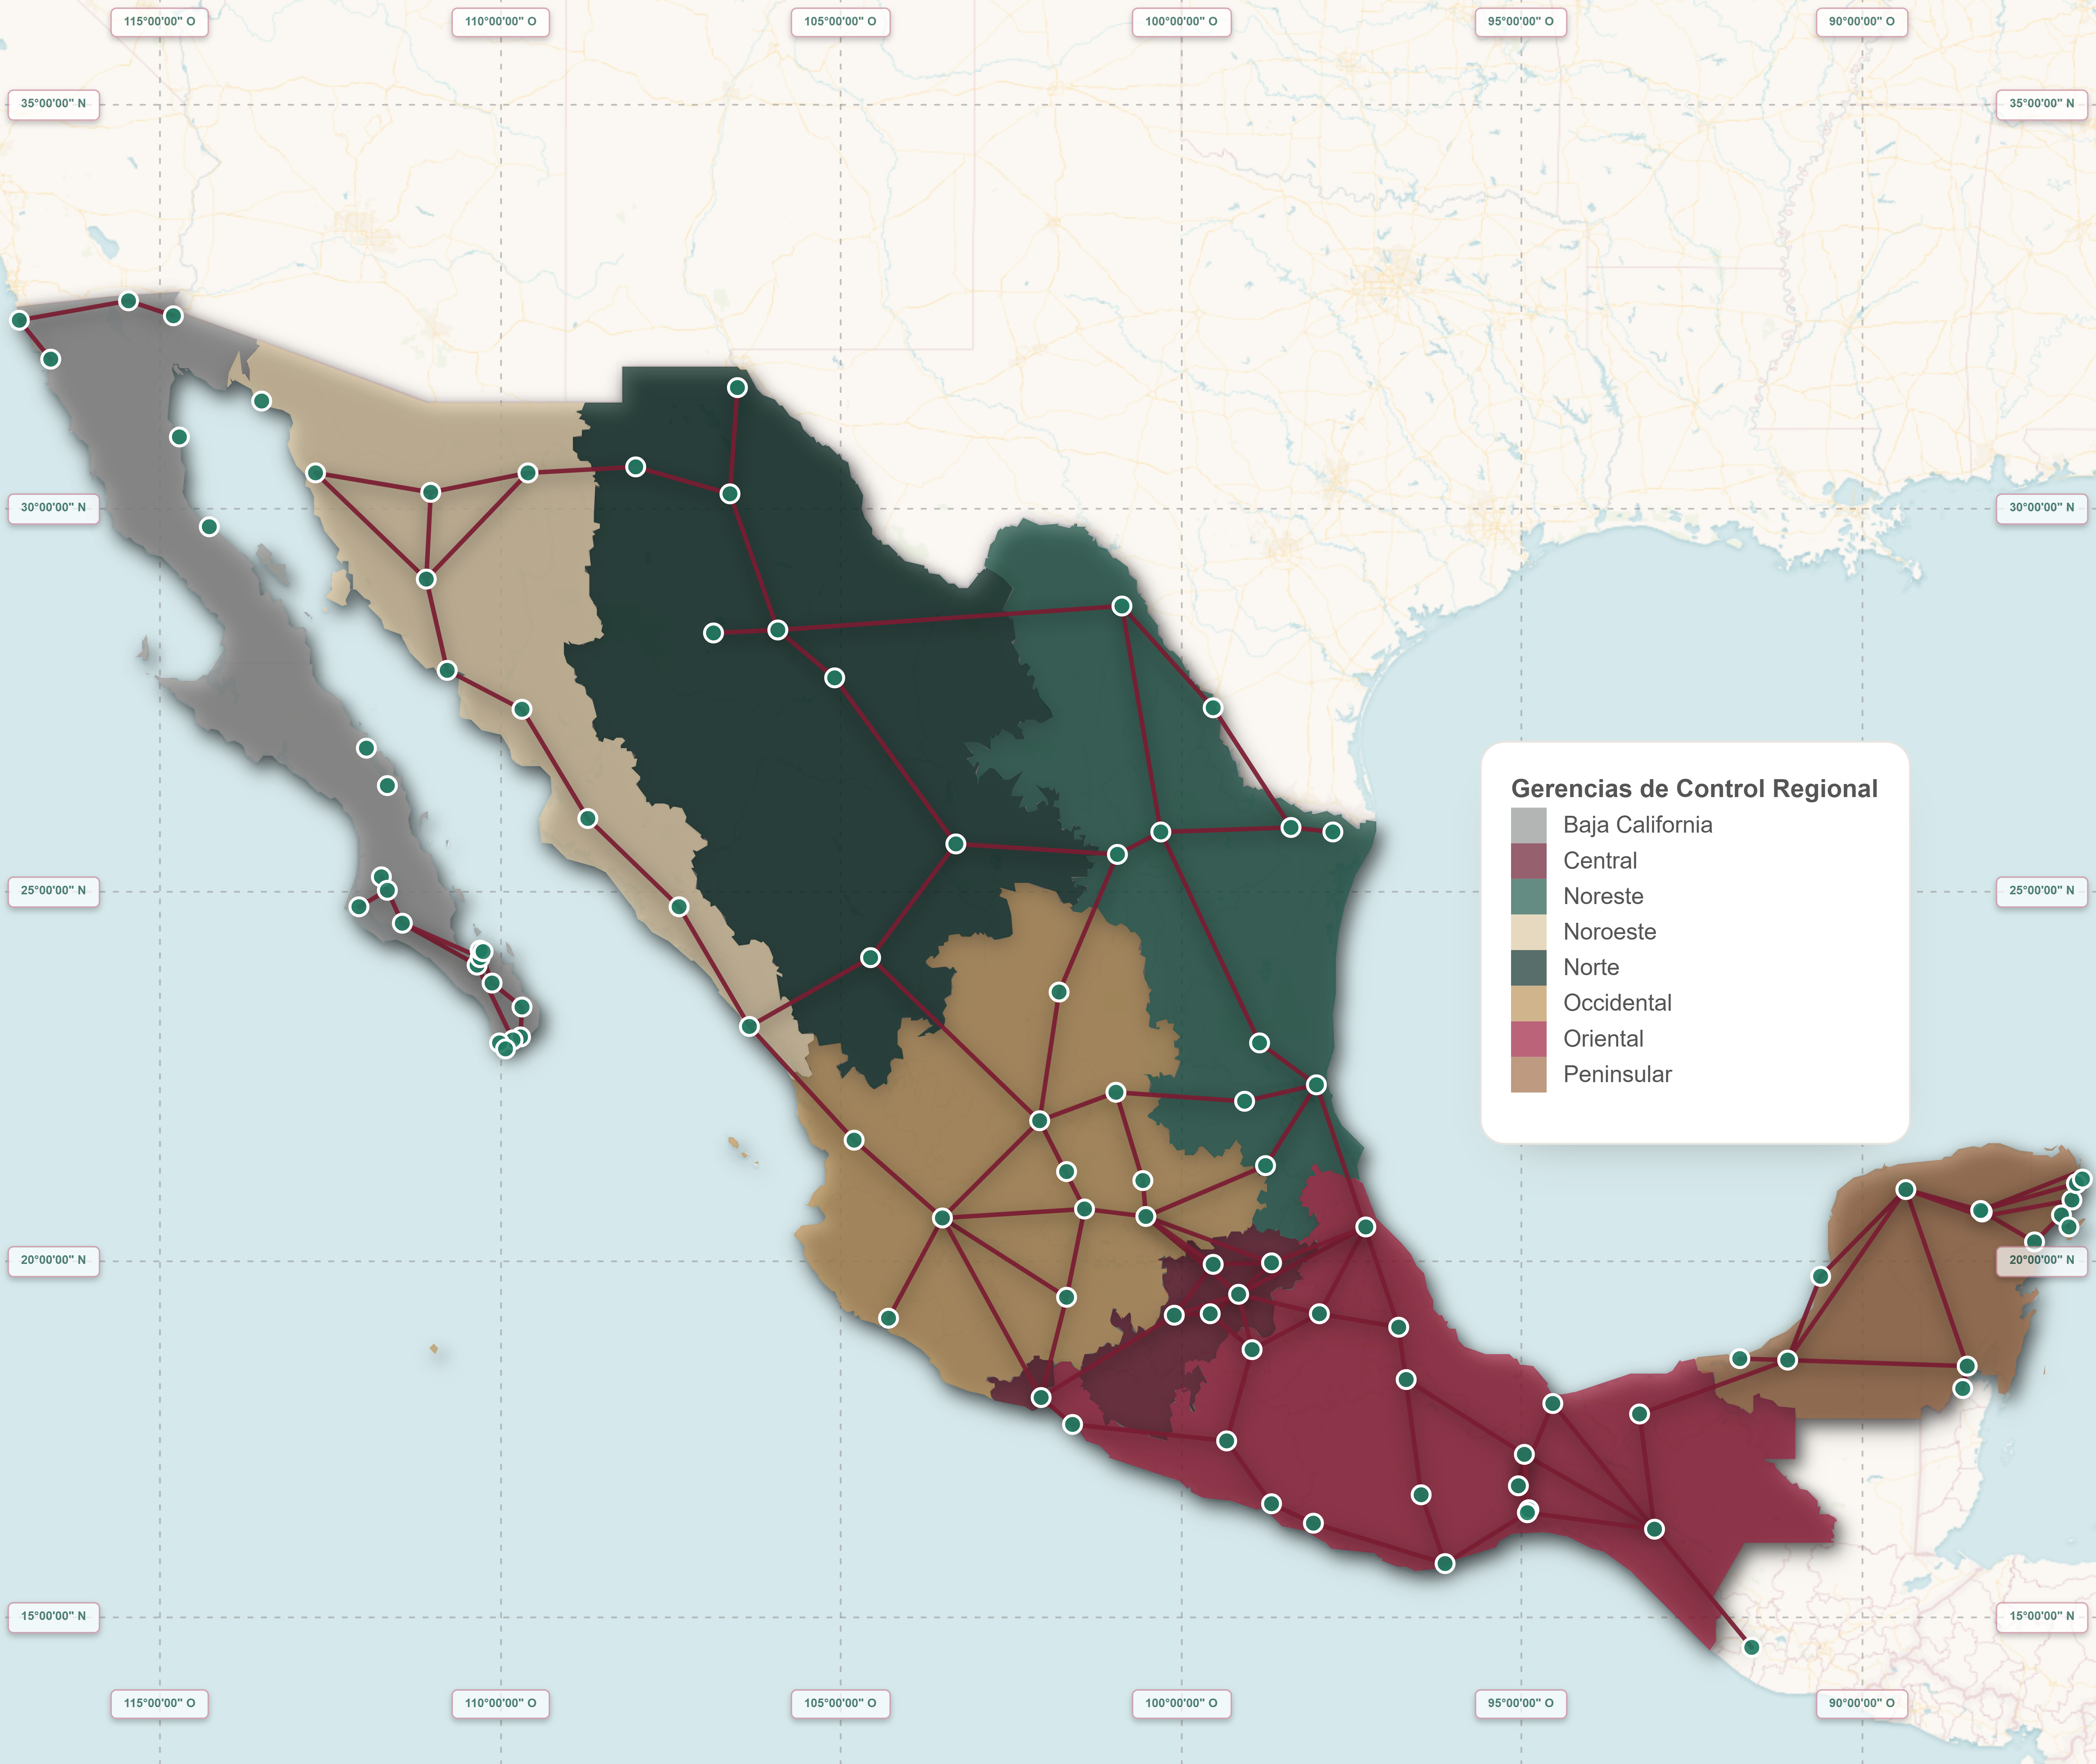
\includegraphics[width=1.0\textwidth]{img/figura_2_1.png}}{Figura 2.1. Provincia Petroleras de la República Mexicana}
  \par}
  \raggedright
  \caption{Figura 2.1. Provincias Petroleras de la República Mexicana}
  \label{fig:FIG-2.1.1-1}
\end{figure}
\vspace{-4pt}
\fuente{Elaboración SENER.}


Los pozos exploratorios son perforados con la finalidad de confirmar el potencial geológico y la presencia de hidrocarburos en nuevas áreas de interés. Entre 2010 y 2024 se perforaron 557 pozos exploratorios en el país, de los cuales PEMEX perforó el 81\%, mientras que los contratistas realizaron el 19\% restante. La actividad estuvo dominada por PEMEX a lo largo del periodo, con un repunte significativo entre 2021 y 2023, lo que refleja la reactivación exploratoria tras la pandemia generada por el virus SARS-CoV-2, así como el impulso a los proyectos exploratorios orientados a mantener tasas de incorporación de reservas acordes con la plataforma de producción (Figura 2.2).

\Needspace{18\baselineskip}
\begin{figure}[H]
  {\centering
  % Texto alternativo para accesibilidad
  \pdftooltip{\includegraphics[width=1.0\textwidth]{img/figura_2_2.png}}{Figura 2.2. Número de pozos exploratorios perforados por tipo de Operador}
  \par}
  \raggedright
  \caption{Figura 2.2. Número de pozos exploratorios perforados por tipo de Operador}
  \label{fig:FIG-2.1.1-2}
\end{figure}
\vspace{-4pt}
\fuente{Sistema de Información de Hidrocarburos - SENER.   Nota: Considera pozos delimitadores y evaluadores.}


A través de la evolución de esta actividad (Figura 2.3) puede observarse la dinámica anual de perforación de pozos exploratorios en el periodo 2010-2024.

A partir de 2019, en sintonía con la política energética orientada a fortalecer la autosuficiencia y priorizar el desarrollo de áreas petroleras en aguas someras y terrestres, se observó un repunte en la perforación de pozos exploratorios en las Cuencas del Sureste, principalmente en aguas someras. Asimismo, se fortalecieron las actividades exploratorias en las Provincias Petroleras de Burgos, Veracruz y Tampico-Misantla, regiones con alto potencial gasífero. Esta reactivación responde al objetivo de reducir la dependencia de importaciones de gas natural y aprovechar las reservas disponibles.

\Needspace{18\baselineskip}
\begin{figure}[H]
  {\centering
  % Texto alternativo para accesibilidad
  \pdftooltip{\includegraphics[width=1.0\textwidth]{img/figura_2_3.png}}{Figura 2.3. pozos exploratorios perforados por Provincia Petrolera}
  \par}
  \raggedright
  \caption{Figura 2.3. Pozos exploratorios perforados por Provincia Petrolera}
  \label{fig:FIG-2.1.1-3}
\end{figure}
\vspace{-4pt}
\fuente{Sistema de Información de Hidrocarburos - SENER.}


En la Tabla 2.1 se presenta la distribución de los pozos exploratorios perforados por provincia petrolera y tipo de operador en el periodo 2010–2024. Se observa que las Cuencas del Sureste concentraron la mayor actividad exploratoria, con 310 pozos, equivalente al 56\% del total nacional, seguida por el Golfo de México Profundo con 82 pozos (15\%) y la Cuenca de Burgos con 54 pozos (10\%). En conjunto, estas tres provincias registraron más del 80\% de la actividad exploratoria registrada durante el periodo.

\begin{tabladoradoCorto}
  \caption{Tabla 2.1 POZOS EXPLORATORIOS PERFORADOS 2010-2024}
  \label{tab:TBL-2.1.1-1}
  \renewcommand{\SENERLongTableFont}{\tiny\sffamily\color{black}}
  {\SENERLongTableFont
  \begin{xltabular}{\textwidth}{p{3cm}*{3}{X}}
    \rowcolor{gobmxDorado}\textcolor{white}{\bfseries CUENCA } & \textcolor{white}{\bfseries PEMEX} & \textcolor{white}{\bfseries CONTRATISTAS} & \textcolor{white}{\bfseries TOTAL GENERAL} \\
    \hline
    \rowcolor{white}Burgos & 40 & 14 & \cellcolor{gobmxDorado!15}{54} \\
    \rowcolor{gray!8}Cinturón Plegado de Chiapas & 3 & 2 & \cellcolor{gobmxDorado!15}{5} \\
    \rowcolor{white}Cuencas del Sureste & 260 & 50 & \cellcolor{gobmxDorado!15}{310} \\
    \rowcolor{gray!8}Golfo de México Profundo & 53 & 29 & \cellcolor{gobmxDorado!15}{82} \\
    \rowcolor{white}Plataforma de Yucatán & 1 &  & \cellcolor{gobmxDorado!15}{1} \\
    \rowcolor{gray!8}Sabinas-Burro-Picachos & 14 &  & \cellcolor{gobmxDorado!15}{14} \\
    \rowcolor{white}Tampico-Misantla & 38 & 5 & \cellcolor{gobmxDorado!15}{43} \\
    \rowcolor{gray!8}Veracruz & 43 & 5 & \cellcolor{gobmxDorado!15}{48} \\
    \rowcolor{gray!20}\textbf{Total general} & \textbf{452} & \textbf{105} & \cellcolor{gobmxDorado!25}{\textbf{557}} \\
  \end{xltabular}}
\end{tabladoradoCorto}
\vspace{-4pt}
\fuente{Sistema de Información de Hidrocarburos - SENER.}


La figura 2.4 presenta la distribución espacial de los pozos exploratorios conforme a las provincias petroleras del país. Se observa una marcada concentración en las actividades de las cuencas del sureste, donde se han focalizado los esfuerzos exploratorios debido a su elevada productividad y madurez geológica. En contraste, las provincias Sabina-Burro-Picachos, Plataforma de Yucatán y el Cinturón Plegado de Chiapas han registrado una actividad exploratoria limitada, ejecutada casi exclusivamente por PEMEX, lo que refleja una menor participación privada en las zonas de complejidad estructural o menor desarrollo infraestructura.

Por su parte, los contratistas tuvieron una participación más visible en el Golfo de México Profundo y en las cuencas Burgos, Veracruz y Tampico-Misantla, lo que evidencia un proceso gradual de diversificación regional de la exploración, orientado hacia áreas con mayor complejidad técnica y potencial geológico.

\Needspace{18\baselineskip}
\begin{figure}[H]
  {\centering
  % Texto alternativo para accesibilidad
  \pdftooltip{\includegraphics[width=1.0\textwidth]{img/figura_2_4.png}}{Figura 2.4. Mapa de pozos exploratorios perforados por Provincia Petrolera}
  \par}
  \raggedright
  \caption{Figura 2.4. Mapa de pozos exploratorios perforados por Provincia Petrolera}
  \label{fig:FIG-2.1.1-4}
\end{figure}
\vspace{-4pt}
\fuente{Elaboración SENER.}



\subsubsection{Asignaciones y Áreas Contractuales}

En la última década, la exploración y extracción de hidrocarburos se ha visto condicionada por factores financieros, regulatorios y tecnológicos. Con la Reforma Energética de 2013\footnote{DECRETO por el que se reforman y adicionan diversas disposiciones de la Constitución Política de los Estados Unidos Mexicanos, en Materia de Energía. DOF: 20/12/2013.}, el sector hidrocarburos se abrió a la inversión de empresas privadas y se crearon dos nuevos modelos para la realización de actividades de exploración y extracción de hidrocarburos: las Asignaciones y los Contratos. Al 31 de diciembre de 2024, se encontraban vigentes 412 Asignaciones y 104 Contratos para la Exploración y Extracción de Hidrocarburos (Tabla 2.2).

\begin{tabladoradoCorto}
  \caption{Tabla 2.2 ASIGNACIONES Y CONTRATOS VIGENTES AL 31 DE DICIEMBRE DE 2024}
  \label{tab:TBL-2.1.2-1}
  \renewcommand{\SENERLongTableFont}{\tiny\sffamily\color{black}}
  {\SENERLongTableFont
  \begin{xltabular}{\textwidth}{p{3cm}*{6}{X}}
    \rowcolor{gobmxDorado}\textcolor{white}{\bfseries } & \textcolor{white}{\bfseries ASIGNACIONES} & \textcolor{white}{\bfseries } & \textcolor{white}{\bfseries } & \textcolor{white}{\bfseries CONTRATOS} & \textcolor{white}{\bfseries } & \textcolor{white}{\bfseries } \\
    \hline
    \rowcolor{white}Extracción
(A) & Exploración (AE) & Resguardo
(AR) & Producción Compartida & Licencia & Asociaciones & \cellcolor{gobmxDorado!15}{Migraciones} \\
    \rowcolor{gray!8}258 & 111 & 43 & 29 & 67 & 3 & \cellcolor{gobmxDorado!15}{5} \\
    \rowcolor{white} & TOTAL: & 412 &  &  & TOTAL:  & \cellcolor{gobmxDorado!15}{104} \\
  \end{xltabular}}
\end{tabladoradoCorto}
\vspace{-4pt}
\fuente{Asignaciones Energía SENER; Contratos: Informe Anual 2024 CNH.}


Respecto de la ubicación de las 412 Asignaciones vigentes, 314 son terrestres, 80 se ubican en aguas someras y 18 en aguas profundas (Tabla 2.3).

\begin{tabladoradoCorto}
  \caption{Tabla 2.3 UBICACIÓN DE ASIGNACIONES VIGENTES AL 31 DE DICIEMBRE DE 2024}
  \label{tab:TBL-2.1.2-2}
  \renewcommand{\SENERLongTableFont}{\tiny\sffamily\color{black}}
  {\SENERLongTableFont
  \begin{xltabular}{\textwidth}{p{3cm}*{8}{X}}
    \rowcolor{gobmxDorado}\textcolor{white}{\bfseries UBICACIÓN / PROVINCIA} & \textcolor{white}{\bfseries BURGOS} & \textcolor{white}{\bfseries CINTURÓN PLEGADO DE CHIAPAS} & \textcolor{white}{\bfseries CUENCAS DEL SURESTE} & \textcolor{white}{\bfseries GOLFO DE MÉXICO PROFUNDO} & \textcolor{white}{\bfseries SABINAS BURRO PICACHO} & \textcolor{white}{\bfseries TAMPICO MISANTLA} & \textcolor{white}{\bfseries VERACRUZ} & \textcolor{white}{\bfseries TOTAL} \\
    \hline
    \rowcolor{white}Terrestre & 79 & 2 & 99 & 0 & 2 & 78 & 54 & \cellcolor{gobmxDorado!15}{314} \\
    \rowcolor{gray!8}Aguas Someras & - & - & 70 & 4 & - & 6 & - & \cellcolor{gobmxDorado!15}{80} \\
    \rowcolor{white}Aguas Profundas & - & - & - & 18 & - & - & - & \cellcolor{gobmxDorado!15}{18} \\
    \rowcolor{gray!20}\textbf{Total general} & \textbf{79} & \textbf{2} & \textbf{169} & \textbf{22} & \textbf{2} & \textbf{84} & \textbf{54} & \cellcolor{gobmxDorado!25}{\textbf{412}} \\
  \end{xltabular}}
\end{tabladoradoCorto}
\vspace{-4pt}
\fuente{Asignaciones Energía SENER.}


En cuanto a su distribución geográfica, la Figura 2.5 muestra la ubicación por Provincia Petrolera de las 412 Asignaciones vigentes al 31 de diciembre de 2024.

\Needspace{18\baselineskip}
\begin{figure}[H]
  {\centering
  % Texto alternativo para accesibilidad
  \pdftooltip{\includegraphics[width=1.0\textwidth]{img/figura_2_5.png}}{Figura 2.5. Ubicación de las Asignaciones por Provincia Petrolera}
  \par}
  \raggedright
  \caption{Figura 2.5. Ubicación de las Asignaciones por Provincia Petrolera}
  \label{fig:FIG-2.1.2-1}
\end{figure}
\vspace{-4pt}
\fuente{Elaboración SENER.}


Con la conclusión de las 9 licitaciones públicas internacionales divididas en 3 Rondas y los procesos de Migración y Asociación, se adjudicaron en total 112 contratos. Al 31 de diciembre de 2024, se encontraban vigentes 104 Contratos, manejados por 46 Operadores petroleros y sus socios (ver Tabla 2.4).

\begin{tabladoradoCorto}
  \caption{Tabla 2.4 UBICACIÓN DE CONTRATOS VIGENTES AL 31 DE DICIEMBRE DE 2024}
  \label{tab:TBL-2.1.2-3}
  \renewcommand{\SENERLongTableFont}{\tiny\sffamily\color{black}}
  {\SENERLongTableFont
  \begin{xltabular}{\textwidth}{p{3cm}*{2}{X}}
    \rowcolor{gobmxDorado}\textcolor{white}{\bfseries TIPO DE CONTRATO} & \textcolor{white}{\bfseries UBICACIÓN} & \textcolor{white}{\bfseries NÚMERO DE CONTRATOS} \\
    \hline
    \rowcolor{white}\multirow{2}{=}{Licencia} & Aguas profundas & \cellcolor{gobmxDorado!15}{23} \\
    \rowcolor{gray!8} & Terrestre & \cellcolor{gobmxDorado!15}{48} \\
    \rowcolor{white}\multirow{2}{=}{Producción Compartida} & Aguas someras & \cellcolor{gobmxDorado!15}{30} \\
    \rowcolor{gray!8} & Terrestre & \cellcolor{gobmxDorado!15}{3} \\
    \hline
    \rowcolor{gray!20}\textbf{Total general} & & \textbf{104} \\
  \end{xltabular}}
\end{tabladoradoCorto}
\vspace{-4pt}
\fuente{Informe Anual 2024 CNH.}


La Figura 2.6 muestra la ubicación por provincia petrolera de los 104 contratos vigentes al 31 de diciembre de 2024. Como puede observarse, los contratos se concentran en las provincias petroleras de Cuencas del Sureste, Golfo de México profundo, Tampico-Misantla y Burgos.

\Needspace{18\baselineskip}
\begin{figure}[H]
  {\centering
  % Texto alternativo para accesibilidad
  \pdftooltip{\includegraphics[width=1.0\textwidth]{img/figura_2_6.png}}{Figura 2.6. Ubicación de los Contratos por Provincia Petrolera}
  \par}
  \raggedright
  \caption{Figura 2.6. Ubicación de los Contratos por Provincia Petrolera}
  \label{fig:FIG-2.1.2-2}
\end{figure}
\vspace{-4pt}
\fuente{Elaboración SENER.}



\subsubsection{Reforma Energética 2025: Asignaciones y Contratos}

Derivado de la Reforma Energética de 2025, se promulgó la LSH, reglamentaria de los artículos 25, párrafo quinto y el artículo 27, párrafo séptimo y 28, párrafo cuarto de la Constitución Política de los Estados Unidos Mexicanos, en materia de hidrocarburos. La LSH mandata que la Nación puede llevar a cabo las actividades de Exploración y Extracción de hidrocarburos, asimismo establece en sus artículos 10 y 11 que la SENER es la encargada de otorgar las Asignaciones bajo las modalidades abajo descritas:

1. Asignaciones para el Desarrollo Propio: Acto jurídico administrativo mediante el cual la SENER otorga exclusivamente a PEMEX el derecho para realizar actividades de Exploración y Extracción de Hidrocarburos en el Área de Asignación, por una duración específica, y en la cual realizará las actividades con sus propias capacidades.
2. Asignaciones para el Desarrollo Mixto: Acto jurídico administrativo mediante el cual la SENER otorga exclusivamente a PEMEX el derecho para realizar actividades de Exploración y Extracción de Hidrocarburos en el Área de Asignación, por una duración específica, y en la cual PEMEX complementa sus técnicas, operativas, financieras o de ejecución mediante la asociación con participantes privados. Esta colaboración permite acelerar la ejecución de proyectos, incorporar las tecnologías avanzadas, optimizar costos y mejorar la gestión de riesgos, alineándose con los objetivos del Plan Nacional de Desarrollo en materia de seguridad energética, sostenibilidad y competitividad.

Mediante las Asignaciones para el Desarrollo Mixto, los privados pueden participar en los proyectos de exploración y extracción con PEMEX a través de procesos de selección autorizados por su Consejo de Administración, presentando propuestas que demuestren valor agregado en términos de recuperación de reservas, eficiencia operativa y cumplimiento regulatorio. Estas sinergias público-privada fortalecen la capacidad del Estado para fortalecer áreas estratégicas, especialmente aquellas con alta complejidad geológica o requerimientos intensivos de capacitación, contribuyendo al aprovechamiento óptimo del potencial energético nacional.

Por lo que se refiere a las bases para la participación de la iniciativa privada en el sector hidrocarburos, destaca la emisión de reglas claras y predecibles para la selección de participantes en Asignaciones para Desarrollo Mixto con PEMEX en exploración y extracción, desde abril de 2025.

Asimismo, el transitorio Décimo de la LSH establece que las Asignaciones y Contratos para la Exploración y Extracción de Hidrocarburos que se hubieran otorgado o celebrado con anterioridad a la entrada en vigor de la LSH, mantendrán su vigencia en los términos y condiciones con que fueron otorgados, conforme a la LSH y a las disposiciones aplicables vigentes a su otorgamiento.

La implementación de la reforma energética ha avanzado de manera firme y ordenada, alineada con los objetivos de soberanía, seguridad, sostenibilidad, autosuficiencia y justicia energética.


\subsubsection{Potencial Petrolero}

\textbf{\textcolor{gobmxDorado}{2.1.4.1. Recursos Prospectivos}}

Los Recursos Prospectivos totales de la Nación ascienden a 112.9 miles de millones de barriles de petróleo crudo equivalente (MMMbpce) (Figura 2.7), en donde el 43\% corresponde a Recursos Convencionales (48.7 MMMbpce) y el 57\% a los Recursos No Convencionales (64.2 MMMbpce).

Estos 112.9 MMMbpce representan la suma del potencial identificado tanto en petróleo crudo, estimado en 68 mil millones de barriles (MMMb) de petróleo crudo , integrados por 32.1 MMMb de Recursos Convencionales y 35.9 MMMb de Recursos no Convencionales y 224.7 Billones de pies cúbicos\footnote{Se refiere a 1x10$^12$ pies cúbicos.} de gas natural (MMMMpc) estimados como recurso prospectivo, de los cuales 83.2 MMMMpc son Recursos Convencionales y 141.5 MMMMpc Recursos no Convencionales.

\Needspace{18\baselineskip}
\begin{figure}[H]
  {\centering
  % Texto alternativo para accesibilidad
  \pdftooltip{\includegraphics[width=1.0\textwidth]{img/figura_2_7.png}}{Figura 2.7. Volúmenes de petróleo crudo equivalente, petróleo crudo y gas natural estimados en los recursos prospectivos de la Nación}
  \par}
  \raggedright
  \caption{Figura 2.7. Volúmenes de petróleo crudo equivalente, petróleo crudo y gas natural estimados en los recursos prospectivos de la Nación}
  \label{fig:FIG-2.1.4-1}
\end{figure}
\vspace{-4pt}
\fuente{Elaboración SENER.}


PEMEX cuenta con 412 Asignaciones vigentes al 31 de diciembre de 2024, que corresponden a una superficie de 109,578.61 km², distribuidas de la siguiente manera: 111 Asignaciones tipo AE, de los cuales 95 prevén derechos para realizar actividades de exploración y extracción y 16 de ellas solo a actividades de extracción; 258 tipo A con derecho para realizar actividades de extracción y; 43 Asignaciones tipo AR, de las cuales 42 tienen derechos para realizar actividades de extracción y una con actividades exclusivamente de resguardo. Las Asignaciones cuentan con Recursos Prospectivos por 40.5 MMMbpce (14.6 MMMbpce en yacimientos convencionales y 25.9 MMMbpce en yacimientos no convencionales).

De los 104 Contratos para la Exploración y Extracción vigentes al 31 de diciembre de 2024, se estima un volumen de Recursos Prospectivos de 10.4 MMMbpce en yacimientos convencionales y 1.4 MMMbpce en yacimientos no convencionales. Estos Contratos se dividen en 71 de tipo Licencia y 33 de Producción Compartida, cubriendo una superficie total de 71,747.52 km². En cuanto al tipo de actividades que se desarrollan, 74 están en la fase de Exploración y Extracción, mientras que los restantes 30 se encuentran sólo realizando actividades de Extracción.

El Estado cuenta con 183 áreas en resguardo, las cuales no han sido asignadas a PEMEX o Contratistas, que poseen un recurso prospectivo de 60.6 MMMbpce, que se distribuyen 23.7 MMMbpce en yacimientos convencionales y 36.9 MMMbpce en yacimientos no convencionales, por lo que se cuenta con potencial en Recursos Prospectivos que se pueden explorar y evaluar para la incorporación de Reservas.

La Tabla 2.5 presenta los Recursos Prospectivos en los diferentes tipos de áreas para las actividades de Exploración y Extracción de hidrocarburos al 31 de diciembre de 2024.

\begin{tabladoradoCorto}
  \caption{TABLA 2.5. RECURSOS PROSPECTIVOS CONVENCIONALES Y NO CONVENCIONALES EN ASIGNACIONES, CONTRATOS DE EXPLORACIÓN Y EXTRACCIÓN, Y ÁREAS DEL ESTADO}
  \label{tab:TBL-2.1.4-1}
  \renewcommand{\SENERLongTableFont}{\tiny\sffamily\color{black}}
  {\SENERLongTableFont
  \begin{xltabular}{\textwidth}{p{3cm}*{3}{X}}
    \rowcolor{gobmxDorado}\textcolor{white}{\bfseries DISTRIBUCIÓN DE LOS RECURSOS} & \textcolor{white}{\bfseries ÁREAS} & \textcolor{white}{\bfseries RECURSOS PROSPECTIVOS CONVENCIONALES (MMMbpce) } & \textcolor{white}{\bfseries RECURSOS PROSPECTIVOS NO CONVENCIONALES (MMMbpce)
} \\
    \hline
    \rowcolor{white}Asignaciones & 412 & 14.6 & \cellcolor{gobmxDorado!15}{25.9} \\
    \rowcolor{gray!8}Contratos de Exploración y Extracción & 104 & 10.4 & \cellcolor{gobmxDorado!15}{1.4} \\
    \rowcolor{white}Áreas del Estado & 183 & 23.7 & \cellcolor{gobmxDorado!15}{36.9} \\
  \end{xltabular}}
\end{tabladoradoCorto}
\vspace{-4pt}
\fuente{Elaboración SENER}


Los recursos prospectivos estimados en el orden de 112.9 MMMbpce, representan un volumen potencial equivalente al doble de la producción de hidrocarburos acumulada y documentada desde 1960 al cierre del 2023 (63 MMMbpce). Así mismo las reservas 3P estimadas al 1° de enero de 2024 equivalen a solo una quinta parte de los recursos prospectivos totales de petróleo crudo equivalente actual. Esto evidencia el amplio potencial geológico por explorar y evaluar, así como la importancia estratégica de mantener las actividades exploratorias que posibiliten la incorporación progresiva de reservas, asegurando la disponibilidad futura de hidrocarburos y contribuyendo así a sostener el desarrollo económico de la nación.

\textbf{\textcolor{gobmxDorado}{2.1.4.2. Reservas}}

De acuerdo con la LSH, las reservas se definen como el volumen de hidrocarburos existente en el subsuelo, calculado a una fecha determinada y bajo condiciones atmosféricas, que se estima será producido de manera técnica y económicamente viable, conforme a las premisas económicas aplicables, utilizando cualquiera de los métodos y sistemas de extracción disponibles a la fecha de evaluación\footnote{Ley del Sector Hidrocarburos, Artículo 5, Fracción XLV.}.

De acuerdo con el grado de certidumbre, las reservas se clasifican como reserva 1P, la cual es igual a la reserva probada y tienen 90\% de probabilidad de ser extraída bajo las condiciones técnicas y económicas presentes; la reserva 2P es igual a la agregación de reservas probadas más las reservas probables y cuenta con una probabilidad de al menos 50\% de ser extraída bajo las condiciones presentes; y la reserva 3P que es igual a la agregación de las reservas probadas, más las probables más las posibles y tienen al menos 10\% de probabilidades de ser extraídas.

En 2012, México implementó una regulación asociada a la cuantificación de reservas y certificaciones, conforme a las mejores prácticas y apegándose a las metodologías internacionales del Petroleum Resources Management System (PRMS). La normativa correspondiente al procedimiento de cuantificación y certificación de reservas, ha sufrido reformas en 2017, 2019, 2022 y 2023, a fin de armonizarla con la política energética nacional.

En 2016, derivado de la adopción de la metodología de evaluación y certificación de reservas de la Sociedad de Ingenieros Petroleros (SPE), se observó una disminución en las Reservas de la Nación; asimismo, desde 2018 hasta 2022 el panorama nacional mostró una tendencia a la baja. Esta situación cambió en 2023 y 2024, como resultado de la incorporación de nuevos descubrimientos, actividades de desarrollo y condiciones más favorables tras la revisión de campos en producción.

Al 1 de enero de 2024, México contaba con un volumen de Reservas 3P por 23,146 millones de barriles de petróleo crudo equivalente (MMbpce), del cual, el 60.9\% se encuentra en las Cuencas del Sureste divididos entre el área marina (51.35\%) y la terrestre (9.51\%). A éstas le siguen la provincia Tampico-Misantla con 22.1\% de las reservas y Veracruz con 9.6\%. En menor proporción se encuentran el Golfo de México profundo con 5.8\%, Burgos con 1.6\% y Sabinas-Burro-Picachos con 0.01\% del volumen total de reservas de petróleo crudo equivalente (Figura 2.8).

\Needspace{18\baselineskip}
\begin{figure}[H]
  {\centering
  % Texto alternativo para accesibilidad
  \pdftooltip{\includegraphics[width=1.0\textwidth]{img/figura_2_8.png}}{Figura 2.8. Reservas 3P de petróleo crudo equivalente por Provincia Petrolera}
  \par}
  \raggedright
  \caption{Figura 2.8. Reservas 3P de petróleo crudo equivalente por Provincia Petrolera}
  \label{fig:FIG-2.1.4-2}
\end{figure}
\vspace{-4pt}
\fuente{Elaboración SENER.}


La Figura 2.9 muestra los resultados obtenidos para las reservas correspondientes a las categorías 1P, 2P y 3P para aceite, gas natural y petróleo crudo equivalente, donde la reserva 1P o probada ascendió a 8,383 MMbpce, los cuales 87\% se encuentra en áreas asignadas a PEMEX y 13\% en áreas de Contratos adjudicados en las rondas de licitación; al sumar la reserva probable a la 1P se obtiene la reserva 2P la cual asciende a 15,530 MMbpce, de la cual 86\% corresponde a PEMEX y el restante 14\% a los Contratistas y por último, al sumar la reserva posible se obtiene la reserva 3P la cual asciende a 23,146 MMbpce; 87\% en Asignaciones de PEMEX y 13\% correspondiente a los Contratistas.

\Needspace{18\baselineskip}
\begin{figure}[H]
  {\centering
  % Texto alternativo para accesibilidad
  \pdftooltip{\includegraphics[width=1.0\textwidth]{img/figura_2_9.png}}{Figura 2.9. Reservas de hidrocarburos al 1 de enero de 2024}
  \par}
  \raggedright
  \caption{Figura 2.9. Reservas de hidrocarburos al 1 de enero de 2024}
  \label{fig:FIG-2.1.4-3}
\end{figure}
\vspace{-4pt}
\fuente{Elaboración SENER.}


\textbf{\textcolor{gobmxDorado}{2.1.4.3. Evolución de las Reservas 2010-2024}}

Las Reservas 3P de petróleo crudo equivalente en el periodo de 2010 a 2015 se mantuvieron en un promedio de 42 MMMbpce, en 2016 sufrieron una caída de casi 30\% respecto del año anterior. En 2019, se implementaron estrategias de exploración y extracción para el corto y mediano plazo para detener la declinación natural de los campos y procurar la incorporación de nuevos campos, dando como resultado que, durante el periodo 2019 a 2024 se mantuvieron las Reservas 3P en un promedio de 23 MMMbpce (Figura 2.10).

Entre 2010 y 2018, las reservas de petróleo crudo equivalente se redujeron a una tasa media anual de 6.4\%, lo anterior debido a la acelerada declinación asociada al agotamiento de campos maduros y una menor reposición de las reservas. Por otro lado, durante el periodo 2019-2024, la tasa media de declinación anual (TMDA) se redujo a 1.6\%, debido a una mejor gestión de la producción de los campos y de la incorporación constante de reservas.

\Needspace{18\baselineskip}
\begin{figure}[H]
  {\centering
  % Texto alternativo para accesibilidad
  \pdftooltip{\includegraphics[width=1.0\textwidth]{img/figura_2_10.png}}{Figura 2.10. Histórico de la cuantificación de las reservas de petróleo crudo equivalente}
  \par}
  \raggedright
  \caption{Figura 2.10. Histórico de la cuantificación de las reservas de petróleo crudo equivalente}
  \label{fig:FIG-2.1.4-4}
\end{figure}
\vspace{-4pt}
\fuente{Elaboración SENER.}


Entre 2010 y 2024, las reservas de hidrocarburos líquidos (Figura 2.11), mostraron una tendencia decreciente, al pasar de 30,497 a 16,383 MMb, lo que equivale a una TMDA de 4.3\%. Dicha reducción se debe principalmente al agotamiento natural de los campos maduros. No obstante, a partir de 2019 se implementaron estrategias de incorporación de reservas y desarrollo acelerado de nuevos campos en áreas terrestres y aguas someras, lo que estabilizó los volúmenes de las reservas.

Del total de reservas 3P de la Nación de hidrocarburos líquidos el 38\% corresponde a petróleo pesado y extrapesado (8,911 MMb). Este tipo de petróleo, debido a su alta densidad y viscosidad, presenta mayores retos en cuanto a su extracción y procesamiento en comparación con los petróleos ligeros, lo que plantea tanto desafíos como oportunidades para el sector energético. Para su explotación eficiente, es necesario invertir en tecnologías especializadas y en la mejora de la infraestructura de producción, de proceso y de refinación, lo que podría contribuir a incrementar la capacidad productiva, asegurando el suministro de este recurso en el largo plazo.

\Needspace{18\baselineskip}
\begin{figure}[H]
  {\centering
  % Texto alternativo para accesibilidad
  \pdftooltip{\includegraphics[width=1.0\textwidth]{img/figura_2_11.png}}{Figura 2.11. Histórico reservas probadas, probables y posibles de líquidos (petróleo + condensados) de la Nación}
  \par}
  \raggedright
  \caption{Figura 2.11. Histórico reservas probadas, probables y posibles de líquidos (petróleo + condensados) de la Nación}
  \label{fig:FIG-2.1.4-5}
\end{figure}
\vspace{-4pt}
\fuente{Elaboración SENER.}


En el caso del gas natural, las reservas 3P disminuyeron de 61,236 a 34,858 miles de millones de pies cúbicos (MMMpc) entre 2010 y 2024 (Figura 2.12), lo que representa una TMDA de 3.9\%. Esta tendencia refleja el comportamiento de la producción de gas asociado en campos petroleros y la reducción de inversiones en proyectos. En los años recientes se registra una ligera recuperación, atribuible a la incorporación de nuevos volúmenes en cuencas con potencial de gas.

\Needspace{18\baselineskip}
\begin{figure}[H]
  {\centering
  % Texto alternativo para accesibilidad
  \pdftooltip{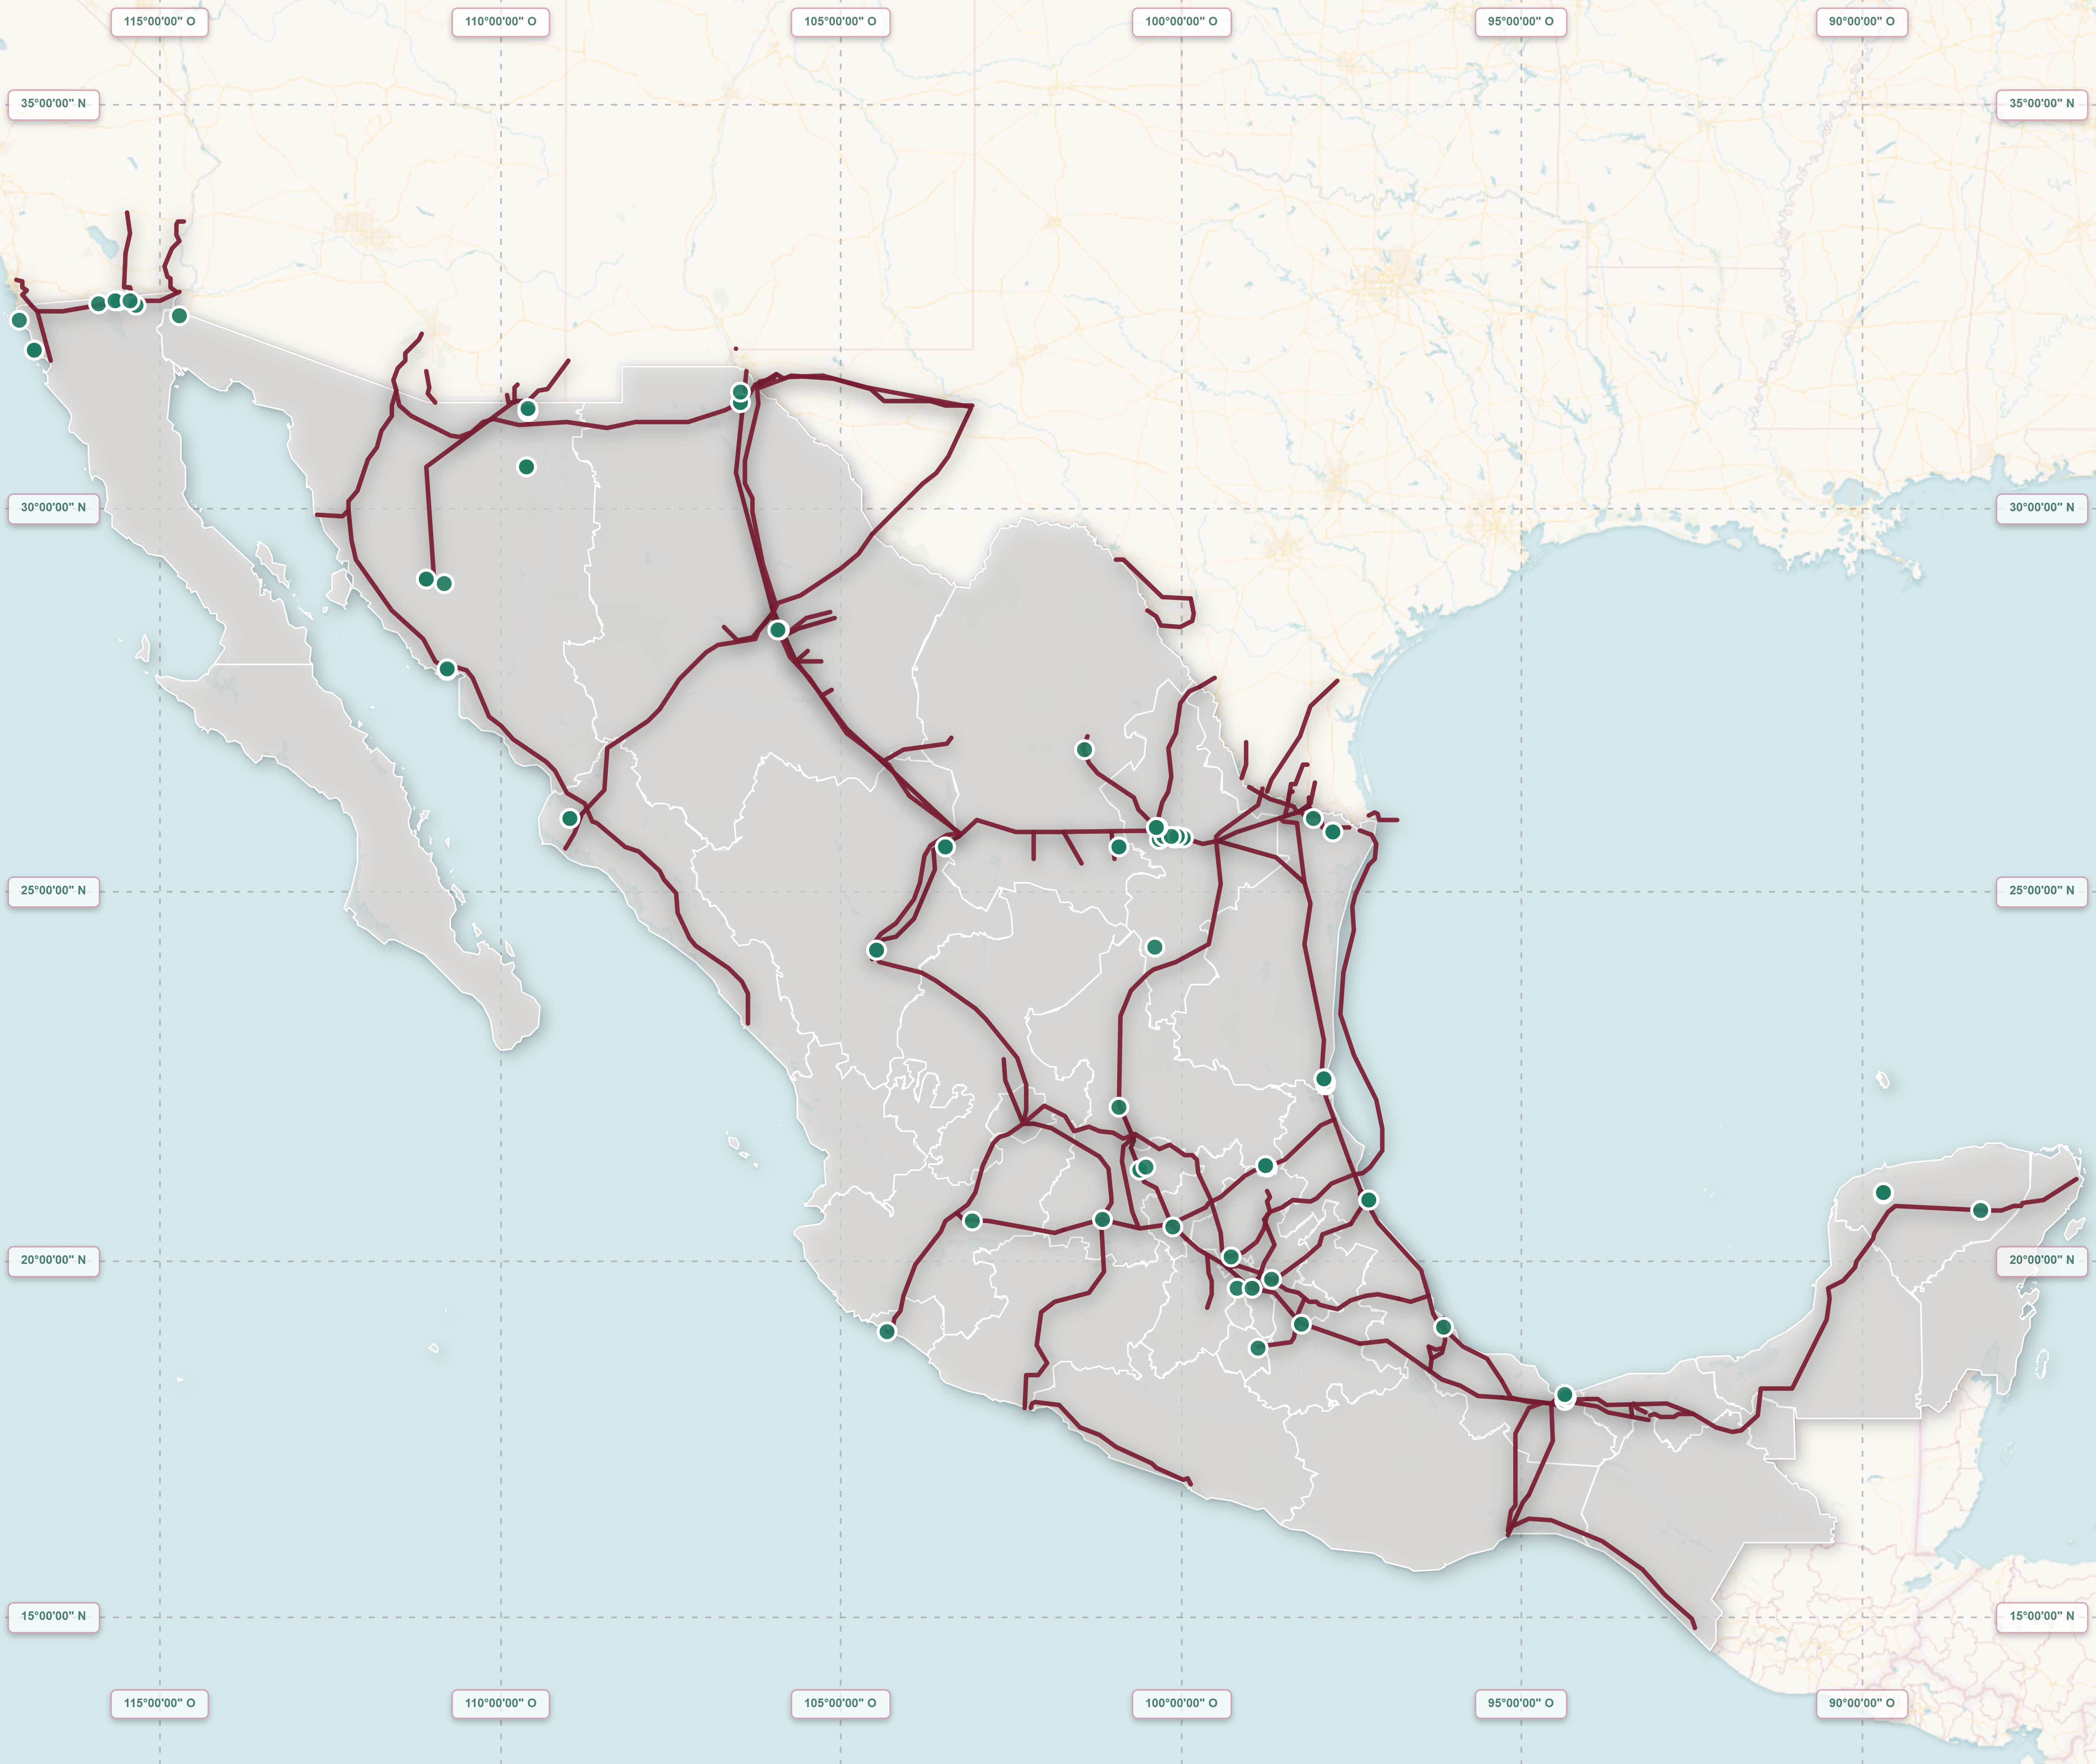
\includegraphics[width=1.0\textwidth]{img/figura_2_12.png}}{Figura 2.12. Histórico reservas probadas, probables y posibles de gas natural de la Nación}
  \par}
  \raggedright
  \caption{Figura 2.12. Histórico reservas probadas, probables y posibles de gas natural de la Nación}
  \label{fig:FIG-2.1.4-6}
\end{figure}
\vspace{-4pt}
\fuente{Elaboración SENER.}


\textbf{\textcolor{gobmxDorado}{2.1.4.4. Descubrimientos comerciales}}

Como resultado de las actividades de exploración, en la cuantificación de Reservas al 1 de enero de 2024 se reportó la incorporación de 12 campos como Descubrimientos Comerciales, además de dos yacimientos adicionales en el campo Vernet. Los descubrimientos comerciales señalados incorporaron reservas al Consolidado Nacional por 33.7 MMbpce en la categoría 1P, 194.8 MMbpce en la categoría 2P y 434.4 MMbpce en la categoría 3P. La Figura 2.13 muestra la localización de los descubrimientos comerciales.

\Needspace{18\baselineskip}
\begin{figure}[H]
  {\centering
  % Texto alternativo para accesibilidad
  \pdftooltip{\includegraphics[width=1.0\textwidth]{img/figura_2_13.png}}{Figura 2.13. Ubicación de los descubrimientos comerciales 2024}
  \par}
  \raggedright
  \caption{Figura 2.13. Ubicación de los descubrimientos comerciales 2024}
  \label{fig:FIG-2.1.4-7}
\end{figure}
\vspace{-4pt}
\fuente{Subsecretaría de Hidrocarburos - SENER.}


Los motivos principales que explican los cambios en las Reservas (al 1 de enero de 2024) se deben a las siguientes causas:

\begin{itemize}
  \item La incorporación del campo Trión en las Reservas 3P de la Nación con 630.2 MMbpce.
  \item La incorporación de Reservas 3P de los campos Bakte, Etkal-NE y Macuil con 172.9 MMbpce, 54.5 MMbpce y 50.4 MMbpce, respectivamente.
  \item El incremento en las Reservas 3P por motivos de revisiones técnicas de los campos Ixachi (con 139.6 MMbpce) y Zaap (94.0 MMbpce).
  \item La reducción en las Reservas 3P del campo Quesqui (en 114.4 MMbpce) por la disminución de presión y producción, así como el campo Ku (en 76.3 MMbpce), debido principalmente a la mayor declinación en la producción por incremento en el corte de agua.
\end{itemize}
En los últimos años, la restitución y el aprovechamiento soberano de los recursos petroleros han representado un desafío estructural en constante adaptación, heredado de un periodo de incertidumbre posterior a la Reforma Energética de 2013, en el que la exploración y el incremento de reservas fueron procesos fragmentados y se desvincularon de los objetivos nacionales. Esto se reflejó en una disminución de las reservas 3P de hidrocarburos líquidos, que pasaron de 30,613 a 19,047 MMb, entre 2012 y 2019.

A partir de 2019 se inició un cambio de rumbo orientado a recuperar la rectoría del Estado, mediante el reordenamiento del portafolio exploratorio y el restablecimiento de una visión de largo plazo sobre las reservas del país. Con la Reforma Energética de 2025, esta transformación se consolida a través de una planeación vinculante establecida en el PLADESHi, en línea con el Plan Nacional de Desarrollo 2025-2030, particularmente con la Estrategia 4.1.4, que impulsa la ampliación sustentable de las reservas de hidrocarburos mediante proyectos estratégicos de exploración y producción. Asimismo, el PROSENER refuerza este enfoque al priorizar el incremento de las reservas 3P para garantizar al menos diez años de consumo nacional, a partir del fortalecimiento de la información geológica y la perforación de pozos exploratorios en proyectos estratégicos ubicados en las principales provincias petroleras del país.


\subsection{Producción}

La producción de hidrocarburos representa el eje central de la cadena de valor del sector hidrocarburos, en donde los recursos previamente descubiertos se transforman en volúmenes comercializables de petróleo y gas natural. Su evolución depende de la dinámica de incorporación de reservas, las estrategias de desarrollo e inversión y la aplicación de nuevas tecnologías para la extracción. La evolución de la producción de hidrocarburos refleja los resultados de las políticas energéticas orientadas a fortalecer la seguridad energética del país. En ese sentido, la producción nacional de hidrocarburos es un componente clave para reducir la dependencia de importaciones y garantizar el suministro estable de petróleo y gas natural.


\subsubsection{Infraestructura de Producción}

\textbf{\textcolor{gobmxDorado}{Pozos de Desarrollo}}

Los pozos de desarrollo tienen como finalidad la puesta en producción de los campos descubiertos. Entre 2010 y 2024 se perforaron un total de 6,030 pozos de desarrollo en el país, de los cuales PEMEX Exploración y Extracción perforó 5,872, y los contratistas han perforado 158 pozos, lo que equivale a 97\% y 3\%, respectivamente (Figura 2.14).

\Needspace{18\baselineskip}
\begin{figure}[H]
  {\centering
  % Texto alternativo para accesibilidad
  \pdftooltip{\includegraphics[width=1.0\textwidth]{img/figura_2_14.png}}{Figura 2.14. Pozos de desarrollo perforados por Operador}
  \par}
  \raggedright
  \caption{Figura 2.14. Pozos de desarrollo perforados por Operador}
  \label{fig:FIG-2.2.1-1}
\end{figure}
\vspace{-4pt}
\fuente{Sistema de Información de Hidrocarburos - SENER.}


La evolución de la perforación de pozos de desarrollo por provincia petrolera en el periodo 2010-2024 puede observarse en la Figura 2.15. Durante dicho periodo, las provincias de Tampico-Misantla y las Cuencas del Sureste concentraron la mayor parte de la actividad de perforaciones de desarrollo con 45\% y 34\% del total, respectivamente. En menor medida, las provincias de Burgos (18\%) y Veracruz (3\%) también registraron actividad de desarrollo, orientada a la producción de gas no asociado.

La estabilización en los niveles de perforación observada a partir de 2019 sugiere una etapa de consolidación en la estrategia de desarrollo, con énfasis en la optimización de la infraestructura existente y el aprovechamiento eficiente de los campos maduros. Cabe señalar, que los esfuerzos por estabilizar los niveles de perforación están alineados con los objetivos de fortalecimiento de la producción nacional establecidos en la política energética vigente.

\Needspace{18\baselineskip}
\begin{figure}[H]
  {\centering
  % Texto alternativo para accesibilidad
  \pdftooltip{\includegraphics[width=1.0\textwidth]{img/figura_2_15.png}}{Figura 2.15. Pozos de desarrollo perforados por Provincia Petrolera}
  \par}
  \raggedright
  \caption{Figura 2.15. Pozos de desarrollo perforados por Provincia Petrolera}
  \label{fig:FIG-2.2.1-2}
\end{figure}
\vspace{-4pt}
\fuente{Sistema de Información de Hidrocarburos - SENER.}


La Figura 2.16 muestra la distribución geográfica de los pozos de desarrollo por provincia petrolera, en la que se observa una mayor concentración de actividades en las Cuencas del Sureste. Particularmente, una mayor concentración de actividades en los campos ubicados en tierra y en aguas someras del litoral de Tabasco y Campeche, regiones que históricamente han aportado la mayor parte de la producción nacional de hidrocarburos.

Asimismo, se observa una presencia importante de pozos en la provincia de Tampico-Misantla, principalmente en el norte de Veracruz y sur de Tamaulipas, donde predominan los proyectos de desarrollo de gas y aceite ligero. En menor medida, las provincias de Burgos y Veracruz registran actividad de desarrollo asociada a la extracción de gas no asociado, mientras que en Sabinas-Burro-Picachos y el Cinturón Plegado de Chiapas la perforación ha sido limitada.

Por su parte los contratistas han mostrado una participación específica en las áreas donde operan los contratos que les fueron adjudicados en las rondas de licitación. La distribución geográfica de los pozos de desarrollo refleja la concentración de las actividades de extracción en zonas de alta madurez geológica y consolidada infraestructura de producción.

\Needspace{18\baselineskip}
\begin{figure}[H]
  {\centering
  % Texto alternativo para accesibilidad
  \pdftooltip{\includegraphics[width=1.0\textwidth]{img/figura_2_16.png}}{Figura 2.16. Pozos de desarrollo perforados por Provincia Petrolera}
  \par}
  \raggedright
  \caption{Figura 2.16. Pozos de desarrollo perforados por Provincia Petrolera}
  \label{fig:FIG-2.2.1-3}
\end{figure}
\vspace{-4pt}
\fuente{Elaboración SENER.}


\textbf{\textcolor{gobmxDorado}{2.2.1.2. Instalaciones de producción}}

Para la realización de las actividades de exploración y extracción, las instalaciones de superficie constituyen un elemento clave para garantizar la operación continua y eficiente de los proyectos. Estas instalaciones permiten llevar a cabo procesos de recolección, separación, compresión, almacenamiento y tratamiento de los hidrocarburos producidos, además de facilitar su transporte hacia los centros de transformación o consumo final.

Con base en la información del Mapa de Hidrocarburos de la SENER, se realizó una agrupación de las principales instalaciones de superficie que se encuentran operando en el territorio nacional, lo anterior considerando su función, la cual que puede ser: recolección y separación, compresión y medición, plantas de proceso, plataformas, almacenamiento y otros.

La Figura 2.17 muestra la distribución de las principales instalaciones de exploración y producción en el territorio nacional, concentrándose principalmente en las Cuencas del Sureste, Tampico-Misantla, Veracruz y Burgos, provincias donde se encuentran los principales campos productores de hidrocarburos de la nación.

\Needspace{18\baselineskip}
\begin{figure}[H]
  {\centering
  % Texto alternativo para accesibilidad
  \pdftooltip{\includegraphics[width=1.0\textwidth]{img/figura_2_17.png}}{Figura 2.17. Instalaciones de exploración y producción}
  \par}
  \raggedright
  \caption{Figura 2.17. Instalaciones de exploración y producción}
  \label{fig:FIG-2.2.1-4}
\end{figure}
\vspace{-4pt}
\fuente{Mapa de Hidrocarburos, SENER.}


\textbf{\textcolor{gobmxDorado}{2.2.1.3. Ductos de Producción de Hidrocarburos}}

La infraestructura de ductos constituye un componente estratégico para la operación eficiente de las actividades de producción, al permitir el transporte de hidrocarburos, fluidos de proceso y agua de inyección entre los distintos centros operativos.

Al 31 de diciembre de 2024, México contaba con una red de aproximadamente 22,288 kilómetros de ductos vinculados a las actividades de producción, conformada principalmente por líneas de descarga (9,397 km), gasoductos (5,518 km), oleoductos (3,041 km), oleogasoductos (2,623 km), además de otros sistemas especializados para el transporte de gasolinas, agua de inyección y bombeo neumático.

La Tabla 2.6 resume la distribución de esta infraestructura por tipo de ducto, donde destaca que el 42\% corresponde a líneas de descarga, 25\% a gasoductos y 14\% a oleoductos.

\begin{tabladoradoCorto}
  \caption{TABLA 2.6. SISTEMAS DE DUCTOS PARA EL MANEJO DE LA PRODUCCIÓN DE HIDROCARBUROS}
  \label{tab:TBL-2.2.1-1}
  \renewcommand{\SENERLongTableFont}{\tiny\sffamily\color{black}}
  {\SENERLongTableFont
  \begin{xltabular}{\textwidth}{p{3cm}*{2}{X}}
    \rowcolor{gobmxDorado}\textcolor{white}{\bfseries TIPO} & \textcolor{white}{\bfseries LONGITUD (KM)} & \textcolor{white}{\bfseries (\%)} \\
    \hline
    \rowcolor{white}Gasoductos & 5,518 & \cellcolor{gobmxDorado!15}{25\%} \\
    \rowcolor{gray!8}Oleoductos & 3,041 & \cellcolor{gobmxDorado!15}{14\%} \\
    \rowcolor{white}Oleogasoductos & 2,623 & \cellcolor{gobmxDorado!15}{12\%} \\
    \rowcolor{gray!8}Gasolinoductos & 337 & \cellcolor{gobmxDorado!15}{2\%} \\
    \rowcolor{white}Ductos de Transporte e Inyección de agua & 190 & \cellcolor{gobmxDorado!15}{1\%} \\
    \rowcolor{gray!8}Líneas de Descarga & 9,397 & \cellcolor{gobmxDorado!15}{42\%} \\
    \rowcolor{white}Líneas de Bombeo Neumático & 989 & \cellcolor{gobmxDorado!15}{4\%} \\
    \rowcolor{gray!8}Otros & 192 & \cellcolor{gobmxDorado!15}{1\%} \\
    \rowcolor{gray!20}\textbf{Total} & \textbf{22,288} & \cellcolor{gobmxDorado!25}{\textbf{100\%}} \\
  \end{xltabular}}
\end{tabladoradoCorto}
\vspace{-4pt}
\fuente{Elaboración SENER}


La Figura 2.18 muestra la distribución espacial de la red de ductos para el manejo de la producción de hidrocarburos, la cual se concentra principalmente en las provincias Cuencas del Sureste, Tampico-Misantla y Burgos. Estas regiones han sostenido históricamente la mayor actividad de extracción y procesamiento de hidrocarburos. La presencia de ductos en dichas áreas responde a la necesidad de transportar grandes volúmenes de petróleo crudo, gas y condensados hacia los complejos de procesamiento y almacenamiento.

\Needspace{18\baselineskip}
\begin{figure}[H]
  {\centering
  % Texto alternativo para accesibilidad
  \pdftooltip{\includegraphics[width=1.0\textwidth]{img/figura_2_18.png}}{Figura 2.18. Sistemas de ductos para el manejo de la producción de hidrocarburos}
  \par}
  \raggedright
  \caption{Figura 2.18. Sistemas de ductos para el manejo de la producción de hidrocarburos}
  \label{fig:FIG-2.2.1-5}
\end{figure}
\vspace{-4pt}
\fuente{Mapa de Hidrocarburos, SENER.}



\subsubsection{Producción de Hidrocarburos}

En 2024, la producción nacional de hidrocarburos líquidos (petróleo crudo más condensados) provino de cuatro provincias petroleras: Cuencas del Sureste, Veracruz, Tampico Misantla y Burgos, de acuerdo con la información reportada por los operadores petroleros. Durante 2024, la producción nacional promedio de líquidos fue de 1,820 miles de barriles diarios (Mbd), cifra 6.0\% menor a la reportada en 2023 de 1,936 Mbd, lo anterior atribuido principalmente a la declinación natural de los campos maduros de las Cuencas del Sureste (Tabla 2.7).

\begin{tabladoradoCorto}
  \caption{TABLA 2.7. PRODUCCIÓN DE HIDROCARBUROS LÍQUIDOS POR PROVINCIA PETROLERA}
  \label{tab:TBL-2.2.2-1}
  \renewcommand{\SENERLongTableFont}{\tiny\sffamily\color{black}}
  {\SENERLongTableFont
  \begin{xltabular}{\textwidth}{p{3cm}*{2}{X}}
    \rowcolor{gobmxDorado}\textcolor{white}{\bfseries PRODUCCIÓN DE HIDROCARBUROS LÍQUIDOS (MBD)} & \textcolor{white}{\bfseries 2023} & \textcolor{white}{\bfseries 2024} \\
    \hline
    \rowcolor{white}Cuencas del Sureste & 1,825 & \cellcolor{gobmxDorado!15}{1,692} \\
    \rowcolor{gray!8}Veracruz & 55 & \cellcolor{gobmxDorado!15}{81} \\
    \rowcolor{white}Tampico Misantla & 54 & \cellcolor{gobmxDorado!15}{47} \\
    \rowcolor{gray!8}Burgos & 2 & \cellcolor{gobmxDorado!15}{1} \\
    \rowcolor{white}Sabinas & - & \cellcolor{gobmxDorado!15}{-} \\
    \rowcolor{gray!20}\textbf{Total} & \textbf{1,936} & \cellcolor{gobmxDorado!25}{\textbf{1,821}} \\
  \end{xltabular}}
\end{tabladoradoCorto}
\vspace{-4pt}
\fuente{Sistema de Información de Hidrocarburos - SENER.}


Durante el año 2024, la producción promedio de hidrocarburos líquidos se concentró en 7 campos operados por PEMEX (Maloob, Zaap, Quesqui, Tupilco Profundo, Ayatsil, Ixachi y Balam). Estos campos aportaron en conjunto el 51\% de la producción nacional de hidrocarburos líquidos en 2024 (Figura 2.19). Destaca el campo Maloob, con una producción promedio de 317 Mbd, equivalente al 17\% de la producción nacional, consolidándose como el principal campo productor de hidrocarburos líquidos del país.

Por su parte, 6 campos operados por contratistas (Hokchi, Amoca, Santuario, Miztón, Pokoch y Tecoalli) contribuyeron con 81.5 Mbd, lo que representa aproximadamente el 4\% del total nacional. Sobresale el campo Hokchi, correspondiente al contrato CNH-R01-L02-A2/2015, operado por Hokchi Energy, S.A. de C.V., con una producción de 21.5 Mbd, equivalente al 1\% del total nacional de hidrocarburos líquidos.

\Needspace{18\baselineskip}
\begin{figure}[H]
  {\centering
  % Texto alternativo para accesibilidad
  \pdftooltip{\includegraphics[width=1.0\textwidth]{img/figura_2_19.png}}{Figura 2.19. Ubicación de los principales campos productores de hidrocarburos líquidos en 2024}
  \par}
  \raggedright
  \caption{Figura 2.19. Ubicación de los principales campos productores de hidrocarburos líquidos en 2024}
  \label{fig:FIG-2.2.2-1}
\end{figure}
\vspace{-4pt}
\fuente{Elaboración SENER.}


La Figura 2.20 muestra la evolución anual de la producción nacional de hidrocarburos líquidos por provincia petrolera para el periodo 2010-2024. Entre 2010 y 2018 la producción nacional de hidrocarburos líquidos mostró una tendencia descendente al pasar de 2,577 Mbd en 2010 a 1,831 Mbd en 2018, lo que equivale a una TMDA de aproximadamente 4\%.

En contraste para el periodo 2019-2024 se observa un cambio en la tendencia de producción registrada en años previos, con una tasa media de crecimiento anual (TMCA) de 1.3\%, resultado de las estrategias de incorporación de reservas y desarrollo acelerado de nuevos campos en áreas terrestres y aguas someras.

\Needspace{18\baselineskip}
\begin{figure}[H]
  {\centering
  % Texto alternativo para accesibilidad
  \pdftooltip{\includegraphics[width=1.0\textwidth]{img/figura_2_20.png}}{Figura 2.20. Producción de hidrocarburos líquidos por Provincia Petrolera}
  \par}
  \raggedright
  \caption{Figura 2.20. Producción de hidrocarburos líquidos por Provincia Petrolera}
  \label{fig:FIG-2.2.2-2}
\end{figure}
\vspace{-4pt}
\fuente{Sistema de Información de Hidrocarburos - SENER.}


La producción de PEMEX representó 94.7\% del total nacional en 2024, con 1,723 Mbd, mientras que los contratistas aportaron 97 Mbd, equivalentes al 5.3\% de la producción nacional. Desde 2017, año en que comenzaron las primeras aportaciones de producción de los contratos adjudicados en las rondas petroleras, la participación de los contratistas ha mostrado un crecimiento gradual, aunque aún marginal frente al volumen de producción de PEMEX (Figura 2.21).

\Needspace{18\baselineskip}
\begin{figure}[H]
  {\centering
  % Texto alternativo para accesibilidad
  \pdftooltip{\includegraphics[width=1.0\textwidth]{img/figura_2_21.png}}{Figura 2.21. Producción de hidrocarburos líquidos por Operador}
  \par}
  \raggedright
  \caption{Figura 2.21. Producción de hidrocarburos líquidos por Operador}
  \label{fig:FIG-2.2.2-3}
\end{figure}
\vspace{-4pt}
\fuente{Sistema de Información de Hidrocarburos - SENER.}



\subsubsection{Producción de Gas natural}

Durante 2024, la producción de gas natural sin nitrógeno se obtuvo de 5 provincias petroleras: Cuencas del Sureste, Veracruz, Burgos, Tampico Misantla y Sabinas, la producción nacional de gas natural sin nitrógeno se situó en 3,760 millones de pies cúbicos diarios (MMpcd), 12.6\% menor a la reportada en 2023 de 4,301 MMpcd (Tabla 2.8).

\begin{tabladoradoCorto}
  \caption{TABLA 2.8. PRODUCCIÓN DE GAS NATURAL POR PROVINCIA}
  \label{tab:TBL-2.2.3-1}
  \renewcommand{\SENERLongTableFont}{\tiny\sffamily\color{black}}
  {\SENERLongTableFont
  \begin{xltabular}{\textwidth}{p{3cm}*{2}{X}}
    \rowcolor{gobmxDorado}\textcolor{white}{\bfseries PRODUCCIÓN DE GAS NATURAL (MMPCD)} & \textcolor{white}{\bfseries 2023} & \textcolor{white}{\bfseries 2024} \\
    \hline
    \rowcolor{white}Cuencas del Sureste & 3,285 & \cellcolor{gobmxDorado!15}{2,653} \\
    \rowcolor{gray!8}Veracruz & 439 & \cellcolor{gobmxDorado!15}{615} \\
    \rowcolor{white}Burgos & 481 & \cellcolor{gobmxDorado!15}{410} \\
    \rowcolor{gray!8}Tampico Misantla & 93 & \cellcolor{gobmxDorado!15}{78} \\
    \rowcolor{white}Sabinas & 4 & \cellcolor{gobmxDorado!15}{3} \\
    \rowcolor{gray!20}\textbf{Total} & \textbf{4,301} & \cellcolor{gobmxDorado!25}{\textbf{3,759}} \\
  \end{xltabular}}
\end{tabladoradoCorto}
\vspace{-4pt}
\fuente{Sistema de Información de Hidrocarburos - SENER.   No incluye Nitrógeno.}


En 2024, la producción promedio de gas natural sin nitrógeno se concentró en 8 campos (Quesqui, Ixachi, Akal, Maloob, Onel, Tupilco Profundo, Koban y Etkal) operados por PEMEX, los cuales representaron en conjunto el 50\% de la producción nacional de gas natural.

El campo Quesqui, aportó durante 2024 una producción promedio de 546 MMpcd (sin nitrógeno), equivalente al 15\% de la producción nacional, consolidándose como el principal campo productor de gas natural del país.

Por otro lado, los contratistas contribuyeron con un total de 191 MMpcd, de los cuales, 5 campos (Arcabuz, Santa Anita, Santuario, Pokoch y Amoca) aportaron en conjunto 102 MMpcd, lo que representa aproximadamente el 4\% del total nacional. Sobresale el campo Arcabuz, correspondiente al contrato CNH-M3-MISIÓN/2018 con una producción de 40.6 MMpcd equivalente al 1\% de la producción nacional de gas natural.

\Needspace{18\baselineskip}
\begin{figure}[H]
  {\centering
  % Texto alternativo para accesibilidad
  \pdftooltip{\includegraphics[width=1.0\textwidth]{img/figura_2_22.png}}{Figura 2.22. Ubicación de los principales campos productores de gas natural en 2024}
  \par}
  \raggedright
  \caption{Figura 2.22. Ubicación de los principales campos productores de gas natural en 2024}
  \label{fig:FIG-2.2.3-1}
\end{figure}
\vspace{-4pt}
\fuente{Elaboración SENER.}


La Figura 2.23 muestra la evolución anual de la producción nacional de gas natural sin nitrógeno por provincia petrolera para el periodo 2010-2024. La producción nacional tuvo una tendencia descendente al pasar de 6,337 MMpcd en 2010 a 3,705 MMpcd en 2018, lo que equivale a una TMDA de 6.49\%.

Dada la importancia del gas natural para la seguridad y soberanía energética del país, a partir de 2019 se impulsaron proyectos estratégicos para el desarrollo de Ixachi y Quesqui, con el objetivo de incrementar la producción de gas no asociado, lo anterior resultó en un cambio en la tendencia de producción de gas natural, para el periodo 2019-2024 se observa una estabilización de la producción, resultando en una TMDA de 0.24\%.

\Needspace{18\baselineskip}
\begin{figure}[H]
  {\centering
  % Texto alternativo para accesibilidad
  \pdftooltip{\includegraphics[width=1.0\textwidth]{img/figura_2_23.png}}{Figura 2.23. Producción gas natural por Provincia Petrolera}
  \par}
  \raggedright
  \caption{Figura 2.23. Producción gas natural por Provincia Petrolera}
  \label{fig:FIG-2.2.3-2}
\end{figure}
\vspace{-4pt}
\fuente{Sistema de Información de Hidrocarburos - SENER.}


La producción de gas natural sin nitrógeno de PEMEX representó el 95\% (3,569 MMpcd) del total nacional en 2024 (3,760 MMpcd), mientras que los contratistas aportaron 191 MMpcd, equivalentes al 5\% de la producción nacional. Desde 2017, año en que comenzaron las primeras aportaciones de los contratos adjudicados en las rondas petroleras, la participación de los contratistas ha mostrado un crecimiento gradual, aunque aún marginal frente al volumen de producción de PEMEX (Figura 2.24).

\Needspace{18\baselineskip}
\begin{figure}[H]
  {\centering
  % Texto alternativo para accesibilidad
  \pdftooltip{\includegraphics[width=1.0\textwidth]{img/figura_2_24.png}}{Figura 2.24. Producción de gas natural por Operador}
  \par}
  \raggedright
  \caption{Figura 2.24. Producción de gas natural por Operador}
  \label{fig:FIG-2.2.3-3}
\end{figure}
\vspace{-4pt}
\fuente{Sistema de Información de Hidrocarburos - SENER.}


La evolución de la producción nacional de hidrocarburos refleja los efectos de un modelo que, durante varios años, subordinó los horizontes productivos a criterios de corto plazo y fragmentó la conducción del sector. Tras la Reforma Energética de 2013, se registró una caída sostenida en la producción de hidrocarburos líquidos, al pasar de 2,522 Mbd en 2013 a 1,705 Mbd en 2019, así como en la producción de gas natural, que disminuyó de 5,679 MMpcd a 3,806 MMpcd en el mismo periodo. Esta tendencia evidenció la ausencia de una estrategia integral para sostener la extracción, compensar la declinación natural de los campos y articular la producción con los objetivos de seguridad energética y desarrollo nacional. Como resultado, se debilitó la capacidad del Estado para garantizar el abasto interno y aumentó la dependencia respecto del exterior.

A partir de 2019, la política energética inició un proceso de reordenamiento productivo orientado a recuperar la rectoría del Estado sobre la producción de hidrocarburos, fortalecer a Pemex y priorizar el desarrollo de campos estratégicos, particularmente aquellos con mayor rentabilidad y solidez técnica. Este viraje permitió avanzar hacia la estabilización de la producción y sentar las bases para una gestión más eficiente y planificada de los recursos del subsuelo.

Con la Reforma Energética de 2025, se consolida mediante un nuevo modelo energético cuya planeación es vinculante y articula de manera integral la exploración y la extracción, con el fin de cumplir las metas de producción establecidas en el Objetivo 1 del Plan Nacional de Desarrollo 2025-2030 y en las líneas de acción del Plan México para alcanzar 1.8 millones de barriles diarios de hidrocarburos líquidos y 5,000 MMpcd. El nuevo marco normativo reconoce a la producción de hidrocarburos como una actividad estratégica que fortalece la soberanía energética y asegura el aprovechamiento de los recursos nacionales bajo criterios de sustentabilidad, eficiencia operativa y beneficio directo para el desarrollo nacional.


\subsection{Evolución de la Transformación de Hidrocarburos}

La industria de transformación comprende una serie de procesos físicos y químicos a los que se someten el petróleo crudo y el gas natural para obtener por destilación y procesos químicos, los diversos hidrocarburos, petrolíferos o petroquímicos. PEMEX, es la encargada de las actividades relacionadas con la transformación de hidrocarburos en el país.

México cuenta con una extensa infraestructura para la transformación de hidrocarburos como Refinerías, Complejos Procesadores de Gas (CPG) y Complejos Petroquímicos (CPQ).


\subsubsection{Refinación}

El petróleo crudo debe someterse a un conjunto de procesos físicos y químicos que lo transforman en productos derivados, como gasolinas, naftas, querosenos, gasóleos, butanos, entre otros. A este proceso se le conoce como refinación.

Las refinerías son los centros de trabajo en los que se llevan a cabo procesos como destilación, hidrodesulfuración, desintegración, entre otros, con la finalidad de transformar el petróleo en sus derivados.

El Sistema Nacional de Refinación (SNR) de México está conformado por un conjunto de refinerías estratégicamente ubicadas en el territorio nacional, cuya operación tiene como propósito transformar el crudo nacional en petrolíferos con la finalidad de atender la demanda interna, (Figura 2.25).

\Needspace{18\baselineskip}
\begin{figure}[H]
  {\centering
  % Texto alternativo para accesibilidad
  \pdftooltip{\includegraphics[width=1.0\textwidth]{img/figura_2_25.png}}{Figura 2.25. Ubicación de refinerías del Sistema Nacional de Refinación}
  \par}
  \raggedright
  \caption{Figura 2.25. Ubicación de refinerías del Sistema Nacional de Refinación}
  \label{fig:FIG-2.3.1-1}
\end{figure}
\vspace{-4pt}
\fuente{Elaboración SENER.}


Durante los últimos años, el SNR integrado por siete refinerías, cuatro de ellas con configuración de coquización (procesamiento de crudos pesados) y tres con configuración de craqueo catalítico (procesamiento de crudos ligeros), había presentado una caída sostenida en el procesamiento de crudo, y consecuente rezago en el mantenimiento de la Infraestructura de las refinerías; principalmente a la atención del rezago en reparaciones mayores y fallas recurrente en equipos estáticos y dinámicos, asociadas en primera instancia a la falta de recursos financieros oportunos para la contratación y la ejecución de las reparaciones requeridas, (Tabla 2.9).

\begin{tabladoradoCorto}
  \caption{TABLA 2.9. INICIO DE OPERACIONES POR REFINERÍA}
  \label{tab:TBL-2.3.1-1}
  \renewcommand{\SENERLongTableFont}{\tiny\sffamily\color{black}}
  {\SENERLongTableFont
  \begin{xltabular}{\textwidth}{p{3cm}*{2}{X}}
    \rowcolor{gobmxDorado}\textcolor{white}{\bfseries REFINERÍA} & \textcolor{white}{\bfseries INICIO DE OPERACIONES} & \textcolor{white}{\bfseries REGIÓN DE ABASTECIMIENTO} \\
    \hline
    \rowcolor{white}Salamanca & 1950 & \cellcolor{gobmxDorado!15}{Centro-Occidente} \\
    \rowcolor{gray!8}Minatitlán & 1956 & \cellcolor{gobmxDorado!15}{Sur-Sureste} \\
    \rowcolor{white}Madero & 1960 & \cellcolor{gobmxDorado!15}{Noreste} \\
    \rowcolor{gray!8}Tula & 1977 & \cellcolor{gobmxDorado!15}{Centro} \\
    \rowcolor{white}Salina Cruz & 1979 & \cellcolor{gobmxDorado!15}{Sur-Sureste} \\
    \rowcolor{gray!8}Cadereyta & 1979 & \cellcolor{gobmxDorado!15}{Noreste} \\
    \rowcolor{white}Olmeca & 2024 & \cellcolor{gobmxDorado!15}{Sureste} \\
  \end{xltabular}}
\end{tabladoradoCorto}
\vspace{-4pt}
\fuente{Elaboración SENER.}


PEMEX, es la empresa pública del estado encargada de ejecutar los procesos industriales para convertir el petróleo crudo y el gas natural en productos de mayor valor en la industria energética y petroquímica en el país.

La visión del Gobierno Federal para el Sector Energético y el subsector hidrocarburos transitó hacia el fortalecimiento de PEMEX como palanca del desarrollo nacional, impulsando su recuperación que le permitiera consolidarse como el instrumento del Estado para alcanzar la soberanía y seguridad energética nacional, y destacando entre otros elementos prioritarios, la rehabilitación de las refinerías existentes.

El SNR cuenta con una capacidad instalada adecuada para procesar la disponibilidad actual de crudo producido en el país y cumplir con las exigencias derivadas de las restricciones ambientales vigentes.

En línea con el objetivo de alcanzar la autosuficiencia energética, en 2022 PEMEX fortaleció su participación en el mercado de petrolíferos mediante la adquisición del 50\% de la participación de Shell respecto de la refinería Deer Park, ubicada en Texas, Estados Unidos, con lo cual obtuvo el 100\% de su propiedad. Deer Park opera bajo control de PEMEX, lo que contribuye al fortalecimiento de su posición estratégica, a la optimización de su portafolio de refinación y al incremento del valor económico de la Empresa Pública del Estado.

El SNR hasta el 2024, contaba con una capacidad instalada de 1,980 Mbd y la refinería Olmeca es la de mayor capacidad (Tabla 2.10).

\begin{tabladoradoCorto}
  \caption{TABLA 2.10. CAPACIDAD DE PROCESO INSTALADA POR REFINERÍA 2024}
  \label{tab:TBL-2.3.1-2}
  \renewcommand{\SENERLongTableFont}{\tiny\sffamily\color{black}}
  {\SENERLongTableFont
  \begin{xltabular}{\textwidth}{p{3cm}*{7}{X}}
    \rowcolor{gobmxDorado}\textcolor{white}{\bfseries CAPACIDAD (MBD)} & \textcolor{white}{\bfseries CADEREYTA} & \textcolor{white}{\bfseries MADERO} & \textcolor{white}{\bfseries OLMECA} & \textcolor{white}{\bfseries MINATITLÁN} & \textcolor{white}{\bfseries SALAMANCA} & \textcolor{white}{\bfseries SALINA CRUZ} & \textcolor{white}{\bfseries TULA} \\
    \hline
    \rowcolor{white}Destilación
Atmosférica & 275 & 190 & 340 & 285 & 245 & 330 & \cellcolor{gobmxDorado!15}{315} \\
    \rowcolor{gray!8}Destilación
al Vacío & 124 & 91 & 176 & 129 & 119 & 165 & \cellcolor{gobmxDorado!15}{144} \\
    \rowcolor{white}Desintegración & 90 & 61 & 94 & 72 & 40 & 80 & \cellcolor{gobmxDorado!15}{80} \\
    \rowcolor{gray!8}Reducción
de Viscosidad & - & - & 130 & - & - & 50 & \cellcolor{gobmxDorado!15}{41} \\
    \rowcolor{white}Reformación
de Naftas & 46 & 30 & 82 & 49 & 39 & 50 & \cellcolor{gobmxDorado!15}{65} \\
    \rowcolor{gray!8}Hidrodesulfuración & 229 & 182 & 350 & 213 & 142 & 215 & \cellcolor{gobmxDorado!15}{249} \\
    \rowcolor{white}Alquilación
e Isomerización & 23 & 22 & 48 & 42 & 14 & 28 & \cellcolor{gobmxDorado!15}{25} \\
    \rowcolor{gray!8}Coquización & 50 & 50 & 130 & 56 & - & - & \cellcolor{gobmxDorado!15}{-} \\
  \end{xltabular}}
\end{tabladoradoCorto}
\vspace{-4pt}
\fuente{Elaboración propia con información de PEMEX.}


El volumen procesado de crudo en el SNR desde el año 2010 y hasta el 2014 se mantuvo por arriba de 1,155 Mbd. Sin embargo, a partir del año 2015, el proceso de crudo en las refinerías comenzó a disminuir a una TMDA del 17.3\%, alcanzando 612 Mbd en el año 2018. Las refinerías pasaron de operar a una capacidad promedio de hasta 76\% a una capacidad promedio del 38\%. Estos cambios en la producción son reflejo de la entrada en vigor de la Reforma Energética del 2013\footnote{DECRETO por el que se reforman y adicionan diversas disposiciones de la Constitución Política de los Estados Unidos Mexicanos, en Materia de Energía. DOF: 20/12/2013.}, la cual alentaba la importación de petrolíferos.

En 2019 se logró detener la caída del proceso de petróleo crudo en las refinerías de PEMEX ubicadas en el territorio nacional y a partir de 2021 y hasta 2024 ha venido creciendo la refinación a una TMCA del 11\%, incrementado la utilización de la capacidad instalada promedio a un 55\%\footnote{No se contabiliza la refinería Olmeca debido a encontrarse en etapa de pruebas de arranque.}, esto derivado de la rehabilitación de las seis refinerías que hasta 2018 no habían recibido el mantenimiento requerido.

En 2024, el SNR procesó un total de 906 Mbd de petróleo crudo\footnote{Las cifras presentadas han sido redondeadas, por lo que pueden existir ligeras variaciones respecto a los valores reales.} (Figura 2.26), lo que representa un incremento de 14\% en comparación con 2023. De acuerdo con el tipo de crudo, durante 2024 se procesó:

\begin{itemize}
  \item 49\% de crudo pesado
  \item 44\% de crudo ligero
  \item 7\% de crudo superligero
\end{itemize}
\Needspace{18\baselineskip}
\begin{figure}[H]
  {\centering
  % Texto alternativo para accesibilidad
  \pdftooltip{\includegraphics[width=1.0\textwidth]{img/figura_2_26.png}}{Figura 2.26. Proceso de crudo anual por refinería 2010-2024}
  \par}
  \raggedright
  \caption{Figura 2.26. Proceso de crudo anual por refinería 2010-2024}
  \label{fig:FIG-2.3.1-2}
\end{figure}
\vspace{-4pt}
\fuente{Elaboración propia con información de PEMEX.}


En 2024, las refinerías de Cadereyta, Madero y Minatitlán procesaron el 63.41\% del crudo pesado, ya que son instalaciones que cuentan con procesos de conversión de residuales. En cambio, en Salamanca, Tula y Salina Cruz se procesó el 74.97\% de crudo ligero.

Derivado del procesamiento de petróleo crudo, el SNR produjo un total de 814 Mbd de petrolíferos\footnote{Solo considera Gasolina, Diésel, Turbosina, Combustóleo y Coque de Petróleo.}, 15\% más que en 2023 (Figura 2.27).

De la producción total de petrolíferos\footnote{Solo considera Gasolina, Diésel, Turbosina, Combustóleo y Coque de Petróleo.}:
\begin{itemize}
  \item 35.61\% se centró en la obtención de Gasolina
  \item 33.35\% en Combustóleo
  \item 22.11\% en Diésel
  \item 4.81\% en Coque de Petróleo
  \item 4.12\% en Turbosina
\end{itemize}
\Needspace{18\baselineskip}
\begin{figure}[H]
  {\centering
  % Texto alternativo para accesibilidad
  \pdftooltip{\includegraphics[width=1.0\textwidth]{img/figura_2_27.png}}{Figura 2.27. Producción de petrolíferos, 2010-2024}
  \par}
  \raggedright
  \caption{Figura 2.27. Producción de petrolíferos*, 2010-2024}
  \label{fig:FIG-2.3.1-3}
\end{figure}
\vspace{-4pt}
{\raggedright\notosanslight\fontsize{7pt}{9pt}\selectfont\setlength{\parskip}{0pt}
* Sólo considera solo la producción de combustóleo, coque de petróleo, diésel, gasolina y turbosina. \par
\vspace{1pt}
{\color{gobmxGris} FUENTE:~Elaboración propia con información de PEMEX.}\hfill
\par}
\vspace{6pt}


Durante 2024, se produjeron 289.85 Mbd de gasolinas, 15\% más comparado con 2023. El 61.60\% de este combustible se obtuvo de las refinerías de Salina Cruz, Tula y Cadereyta.

En 2024 la refinería Olmeca reportó una producción inicial total de 17 Mbd de productos petrolíferos, principalmente diesel y gasolinas, debido a que se encontraba en etapa de pruebas. Al cierre de 2025 se estima una capacidad de procesamiento de 230 Mbd.

La producción de destilados intermedios fue de 179.97 Mbd de diésel y 33.53 Mbd de turbosina. En comparación con 2023, la producción de diésel incrementó 33.48\%, mientras que la de turbosina decreció 7.63\%. Las refinerías de Cadereyta, Minatitlán y Tula concentraron el 56.21\% de la producción de diésel, mientras que la mayor producción de turbosina se registró en Tula y Salina Cruz con el 72.03\% de este petrolífero.

En cuanto a la producción de combustibles residuales, el combustóleo aumentó un 4.28\% de 2023 a 2024. Las refinerías de Salina Cruz, Tula y Salamanca, que están en proceso constructivo para tener equipos de alta conversión de residuales, fueron las de mayor producción de este petrolífero. Por su lado, el coque de petróleo tuvo un aumento del 55.91\% en su producción respecto a 2023.


\subsubsection{Procesamiento de Gas}

El procesamiento de gas natural consiste en un conjunto de operaciones industriales destinadas a separar y purificar los distintos componentes presentes en el gas extraído de yacimientos, con el fin de obtener un producto comercializable que cumpla con las especificaciones del mercado y los requerimientos de transporte.

Además de su infraestructura de refinación, PEMEX cuenta con nueve CPG (Figura 2.28). Estas instalaciones son fundamentales para el procesamiento del gas húmedo, la recuperación de sus componentes ─ como GLP, etano, gasolinas naturales y azufre ─, y su transformación en gas seco o materias primas para la petroquímica, que contribuyen significativamente al suministro energético e industrial del país.

\Needspace{18\baselineskip}
\begin{figure}[H]
  {\centering
  % Texto alternativo para accesibilidad
  \pdftooltip{\includegraphics[width=1.0\textwidth]{img/figura_2_28.png}}{Figura 2.28. Ubicación de los CPG}
  \par}
  \raggedright
  \caption{Figura 2.28. Ubicación de los CPG}
  \label{fig:FIG-2.3.2-1}
\end{figure}
\vspace{-4pt}
\fuente{Elaboración SENER.}


En cuanto a los CPG, siete están ubicados en la región sur-sureste del país y dos en la región noreste. Los complejos de Ciudad Pemex, Cactus y Nuevo Pemex son los más grandes, y en ellos se lleva a cabo el mayor endulzamiento de gas amargo; el procesamiento del gas dulce (recuperación de líquidos) y la recuperación de azufre. En lo que respecta a los condensados, casi la totalidad de su endulzamiento se realiza en los complejos de Cactus y Nuevo Pemex, mientras que buena parte del fraccionamiento de líquidos se lleva a cabo en los complejos de Cactus, Nuevo Pemex y Área Coatzacoalcos, (Tabla 2.11).

\begin{tabladoradoCorto}
  \caption{TABLA 2.11. INICIO DE OPERACIONES POR CPG}
  \label{tab:TBL-2.3.2-1}
  \renewcommand{\SENERLongTableFont}{\tiny\sffamily\color{black}}
  {\SENERLongTableFont
  \begin{xltabular}{\textwidth}{p{3cm}*{2}{X}}
    \rowcolor{gobmxDorado}\textcolor{white}{\bfseries CPG} & \textcolor{white}{\bfseries INICIO DE OPERACIONES} & \textcolor{white}{\bfseries UBICACIÓN} \\
    \hline
    \rowcolor{white}Poza Rica & 1951 & \cellcolor{gobmxDorado!15}{Poza Rica, Veracruz} \\
    \rowcolor{gray!8}Ciudad Pemex & 1958 & \cellcolor{gobmxDorado!15}{Macuspana, Tabasco} \\
    \rowcolor{white}La Venta & 1963 & \cellcolor{gobmxDorado!15}{Huímanguillo, Tabasco} \\
    \rowcolor{gray!8}Cactus & 1974 & \cellcolor{gobmxDorado!15}{Reforma, Chiapas} \\
    \rowcolor{white}Nuevo Pemex & 1976 & \cellcolor{gobmxDorado!15}{Centro, Tabasco} \\
    \rowcolor{gray!8}Matapionche & 1981 & \cellcolor{gobmxDorado!15}{Cotaxtla, Veracruz} \\
    \rowcolor{white}Coatzacoalcos & 1997 & \cellcolor{gobmxDorado!15}{Coatzacoalcos, Veracruz} \\
    \rowcolor{gray!8}Arenque & 2003 & \cellcolor{gobmxDorado!15}{Ciudad Madero, Tamaulipas} \\
    \rowcolor{white}Burgos & 2004 & \cellcolor{gobmxDorado!15}{Reynosa, Tamaulipas} \\
  \end{xltabular}}
\end{tabladoradoCorto}
\vspace{-4pt}
\fuente{Elaboración SENER.}


La SENER realizó un diagnóstico sobre el desempeño de los CPG, en el que se identificó que existía rezago tecnológico en los centros de proceso, falta de competitividad en los procesos operativos respecto de empresas de clase mundial, altos costos de producción, retraso en los programas de mantenimiento y en los trabajos de rehabilitación, y un acelerado incremento de las importaciones de gas natural para cubrir el déficit de la producción.

La actual administración tiene el objetivo de alinear la capacidad de procesamiento con la producción, de modo que la infraestructura existente responda eficientemente al incremento previsto. La estrategia consiste en ampliar la capacidad de los CPG, lo que permitirá manejar de forma segura el gas, garantizando el suministro a los consumidores regionales y, al mismo tiempo, optimizar el uso de la infraestructura, así como fortalecer la confiabilidad operativa del sistema.

Los nueve CPG cuentan con una capacidad instalada de 4,283 MMpcd para el endulzamiento de gas, 135 MMpcd para el tratamiento de líquidos, 5,912 MMpcd para procesos criogénicos, y 560 Mbd para el fraccionamiento de líquidos (Tabla 2.12).

\begin{tabladoradoCorto}
  \caption{TABLA 2.12. CAPACIDAD INSTALADA POR COMPLEJO PROCESADOR DE GAS 2024}
  \label{tab:TBL-2.3.2-2}
  \renewcommand{\SENERLongTableFont}{\tiny\sffamily\color{black}}
  {\SENERLongTableFont
  \begin{xltabular}{\textwidth}{p{3cm}*{4}{X}}
    \rowcolor{gobmxDorado}\textcolor{white}{\bfseries CPG} & \textcolor{white}{\bfseries FRACCIONAMIENTO DE LÍQUIDOS
(MBD)} & \textcolor{white}{\bfseries PLANTAS ENDULZADORAS DE CONDENSANDOS AMARGOS
(MBD)} & \textcolor{white}{\bfseries PLANTAS ENDULZADORAS DE GAS AMARGO
(MMPCD)} & \textcolor{white}{\bfseries PLANTAS RECUPERADORAS DE LICUABLES CRIOGÉNICAS
(MMPCD)} \\
    \hline
    \rowcolor{white}CACTUS & 104 & 45 & 1,800 & \cellcolor{gobmxDorado!15}{1,275} \\
    \rowcolor{gray!8}CIUDAD PEMEX & 0 & 0 & 1,290 & \cellcolor{gobmxDorado!15}{915} \\
    \rowcolor{white}NUEVO PEMEX & 208 & 90 & 800 & \cellcolor{gobmxDorado!15}{1,500} \\
    \rowcolor{gray!8}BURGOS & 18 & 0 & 0 & \cellcolor{gobmxDorado!15}{1,200} \\
    \rowcolor{white}POZA RICA & 22 & 0 & 250 & \cellcolor{gobmxDorado!15}{490} \\
    \rowcolor{gray!8}LA VENTA & 0 & 0 & 0 & \cellcolor{gobmxDorado!15}{182} \\
    \rowcolor{white}ARENQUE & 0 & 0 & 34 & \cellcolor{gobmxDorado!15}{33} \\
    \rowcolor{gray!8}MATAPIONCHE & 0 & 0 & 109 & \cellcolor{gobmxDorado!15}{125} \\
    \rowcolor{white}COATZACOALCOS & 208 & 0 & 0 & \cellcolor{gobmxDorado!15}{192} \\
    \rowcolor{gray!20}\textbf{TOTAL} & \textbf{560} & \textbf{135} & \textbf{4,283} & \cellcolor{gobmxDorado!25}{\textbf{5,912}} \\
  \end{xltabular}}
\end{tabladoradoCorto}
\vspace{-4pt}
\fuente{Elaboración propia con información de PEMEX.}


Derivado de los cambios entre 2012 y 2018, el volumen de gas procesado presentó una disminución asociada principalmente a dos factores: la reducción en la producción nacional de gas natural debido a la declinación de los yacimientos, y la priorización de las importaciones sobre la transformación nacional. Estas acciones se reflejan en una TMDA de 6\%, que resultó en un volumen de 2,952 MMpcd en 2018, equivalente a una reducción del 33\% respecto de 2012 (Figura 2.29).

A partir de 2018, las políticas orientadas a la recuperación de la soberanía energética se enfocaron en frenar el deterioro de la infraestructura dedicada a la transformación de hidrocarburos y en implementar acciones para su rehabilitación. Como resultado, el procesamiento de gas se ha mantenido con una tendencia estable, en 2024 se reportó un volumen procesado de 2,319 MMpcd (Figura 2.29).

Actualmente se desarrollan proyectos dirigidos al incremento de la producción y aprovechamiento del gas natural en los campos, así como programas de ampliación y optimización de la capacidad de procesamiento en los CPG. Cabe destacar que no todo el gas producido es enviado a procesamiento, ya que una parte es tratada y utilizada directamente en plataformas por PEMEX, para reinyectar a los yacimientos, bombeo neumático, combustible o, en su defecto, enviarlo a los quemadores de campo.

\Needspace{18\baselineskip}
\begin{figure}[H]
  {\centering
  % Texto alternativo para accesibilidad
  \pdftooltip{\includegraphics[width=1.0\textwidth]{img/figura_2_29.png}}{Figura 2.29. Proceso de gas natural en los CPG, 2010-2024}
  \par}
  \raggedright
  \caption{Figura 2.29. Proceso de gas natural en los CPG, 2010-2024}
  \label{fig:FIG-2.3.2-2}
\end{figure}
\vspace{-4pt}
\fuente{Elaboración propia con información de PEMEX.}


La producción de gas seco y GLP refleja directamente los volúmenes de insumos que ingresan al proceso. En las gráficas de las figuras 2.30 y 2.31 se observa que durante el periodo 2010–2012 la producción de gas seco en los CPG se mantuvo estable por arriba de 3,600 MMpcd, mientras que la producción de GLP se registró por arriba de los 200 Mbd.

Sin embargo, para el periodo 2012 a 2018 se presenta una TMDA de 6\% para el gas seco y 10\% para el GLP, lo que se traduce en una disminución de la producción de gas seco a 2,418 MMpcd y de GLP a 120 Mbd.

Posteriormente, entre 2018 y 2024, la declinación en la producción se desaceleró, registrando TMDA de 4.5\% para el gas seco y el GLP. Como resultado, en 2024 se reportó una producción de 1,824 MMpcd de gas seco y 92 Mbd de GLP.

\Needspace{18\baselineskip}
\begin{figure}[H]
  {\centering
  % Texto alternativo para accesibilidad
  \pdftooltip{\includegraphics[width=1.0\textwidth]{img/figura_2_30.png}}{Figura 2.30. Producción de gas seco en los CPG, 2010-2024}
  \par}
  \raggedright
  \caption{Figura 2.30. Producción de gas seco en los CPG, 2010-2024}
  \label{fig:FIG-2.3.2-3}
\end{figure}
\vspace{-4pt}
\fuente{Elaboración propia con información de PEMEX.}


\Needspace{18\baselineskip}
\begin{figure}[H]
  {\centering
  % Texto alternativo para accesibilidad
  \pdftooltip{\includegraphics[width=1.0\textwidth]{img/figura_2_31.png}}{Figura 2.31. Producción de GLP en los CPG y SNR, 2010-2024}
  \par}
  \raggedright
  \caption{Figura 2.31. Producción de GLP en los CPG y SNR, 2010-2024}
  \label{fig:FIG-2.3.2-4}
\end{figure}
\vspace{-4pt}
\fuente{Elaboración propia con información de PEMEX.}


El Plan Estratégico 2025–2035 de PEMEX prioriza el fortalecimiento del suministro nacional de gas mediante la incorporación de nuevos desarrollos y proyectos estratégicos en campos terrestres y en aguas profundas que permitirán incrementar la disponibilidad de gas en el periodo 2026–2035.


\subsubsection{Petroquímica}

La petroquímica es la industria que convierte el gas natural y los derivados del petróleo en materias primas para una amplia gama de cadenas productivas, desde la fabricación de fertilizantes, plásticos, resinas y fibras sintéticas, hasta la elaboración de detergentes, solventes, productos farmacéuticos, entre otros. Por ello, la petroquímica es una industria clave para el desarrollo y la competitividad económica del país.

En México, la mayor parte de los petroquímicos son producidos por PEMEX\footnote{En México existe un CPQ privado perteneciente a Grupo IDESA.} , quien cuenta con ocho Complejos Petroquímicos (CPQ), de los cuales actualmente están activos cuatro: La Cangrejera, Cosoleacaque, Morelos e Independencia (Figura 2.32). Los cuatro CPQ que permanecen fuera de operación son Camargo, Pajaritos, Tula y Escolín, los cuales registraron su última producción entre 2002 y 2013. Se tienen programadas acciones de rehabilitación en algunos de los CPQ que se encuentran fuera de operación.

\Needspace{18\baselineskip}
\begin{figure}[H]
  {\centering
  % Texto alternativo para accesibilidad
  \pdftooltip{\includegraphics[width=1.0\textwidth]{img/figura_2_32.png}}{Figura 2.32. Ubicación de los Complejos Petroquímicos}
  \par}
  \raggedright
  \caption{Figura 2.32. Ubicación de los Complejos Petroquímicos}
  \label{fig:FIG-2.3.3-1}
\end{figure}
\vspace{-4pt}
\fuente{Elaboración SENER.}


La desaceleración que ha experimentado la industria petroquímica, no es algo reciente, sino que se remonta al pasado, principalmente con el intento de privatizar PEMEX. En administraciones pasadas no se invirtió en este segmento, principalmente porque no generaba rendimientos inmediatos como la extracción de petróleo, sin embargo, a largo plazo es un sector crítico (Tabla 2.13).

\begin{tabladoradoCorto}
  \caption{TABLA 2.13. INICIO DE OPERACIONES POR CPQ}
  \label{tab:TBL-2.3.3-1}
  \renewcommand{\SENERLongTableFont}{\tiny\sffamily\color{black}}
  {\SENERLongTableFont
  \begin{xltabular}{\textwidth}{p{3cm}*{1}{X}}
    \rowcolor{gobmxDorado}\textcolor{white}{\bfseries CPQ} & \textcolor{white}{\bfseries INICIO DE OPERACIONES} \\
    \hline
    \rowcolor{white}Independencia & \cellcolor{gobmxDorado!15}{1969} \\
    \rowcolor{gray!8}Cosoleacaque & \cellcolor{gobmxDorado!15}{1971} \\
    \rowcolor{white}La Cangrejera & \cellcolor{gobmxDorado!15}{1980} \\
    \rowcolor{gray!8}Morelos & \cellcolor{gobmxDorado!15}{1990} \\
  \end{xltabular}}
\end{tabladoradoCorto}
\vspace{-4pt}
\fuente{Elaboración SENER.}


Al disminuir la inversión, se disminuyó el suministro de materias primas, y con ello la producción de petroquímicos precursores, fue entonces cuando la parte privada de la industria, para poder subsistir, comenzó a sustituir la producción nacional por importaciones de productos petroquímicos.

La industria petroquímica apoya el desarrollo y el crecimiento de México, así como la conformación de cadenas productivas. Esta industria abastece a distintas ramas de la actividad industrial y demanda bienes y servicios de diferentes industrias. Hasta finales de 2024 la capacidad instalada de estos CPQ era de 9,491 miles de toneladas (Tabla 2.14).

\begin{tabladoradoCorto}
  \caption{TABLA 2.14. CAPACIDAD NOMINAL POR CPQ 2024}
  \label{tab:TBL-2.3.3-2}
  \renewcommand{\SENERLongTableFont}{\tiny\sffamily\color{black}}
  {\SENERLongTableFont
  \begin{xltabular}{\textwidth}{p{3cm}*{4}{X}}
    \rowcolor{gobmxDorado}\textcolor{white}{\bfseries CAPACIDAD (Mt)} & \textcolor{white}{\bfseries LA CANGREJERA} & \textcolor{white}{\bfseries COSOLEACAQUE} & \textcolor{white}{\bfseries MORELOS} & \textcolor{white}{\bfseries INDEPENDENCIA} \\
    \hline
    \rowcolor{white}Línea de Aromáticos & 1,342 & 0 & 0 & \cellcolor{gobmxDorado!15}{0} \\
    \rowcolor{gray!8}Estireno & 150 & 0 & 0 & \cellcolor{gobmxDorado!15}{0} \\
    \rowcolor{white}Especialidades Petroquímicas & 0 & 0 & 0 & \cellcolor{gobmxDorado!15}{15} \\
    \rowcolor{gray!8}Metanol & 0 & 0 & 0 & \cellcolor{gobmxDorado!15}{168} \\
    \rowcolor{white}Etileno & 689 & 0 & 655 & \cellcolor{gobmxDorado!15}{0} \\
    \rowcolor{gray!8}Polietileno & 315 & 0 & 502 & \cellcolor{gobmxDorado!15}{0} \\
    \rowcolor{white}Óxido de Etileno & 130 & 0 & 541 & \cellcolor{gobmxDorado!15}{0} \\
    \rowcolor{gray!8}Oxígeno & 192 & 0 & 483 & \cellcolor{gobmxDorado!15}{0} \\
    \rowcolor{white}Acrilonitrilo & 0 & 0 & 96 & \cellcolor{gobmxDorado!15}{0} \\
    \rowcolor{gray!8}Amoniaco & 0 & 4,213 & 0 & \cellcolor{gobmxDorado!15}{0} \\
    \rowcolor{gray!20}\textbf{TOTAL} & \textbf{2,818} & \textbf{4,213} & \textbf{2,277} & \cellcolor{gobmxDorado!25}{\textbf{183}} \\
  \end{xltabular}}
\end{tabladoradoCorto}
\vspace{-4pt}
\fuente{Elaboración propia con información de PEMEX.}


De 2010 a 2018 el abandono de la industria petroquímica se ve reflejado directamente en la producción de productos petroquímicos, ya que tuvo una TMDA del 11\%, pasando de 8,333 miles de toneladas anuales (MTA) en 2010 a 3,331 MTA en 2018, lo que significó una reducción del 60\% de la producción en dicho periodo. Sin embargo, desde 2018, las políticas de recuperación de la soberanía y seguridad energética impulsaron la recuperación de la industria petroquímica, frenando la tendencia decreciente e impulsando nuevamente su crecimiento. En 2024 se alcanzó una producción de 2,373 MTA, 16\% mayor en comparación con 2023 (Figura 2.33 y Figura 2.34).

\Needspace{18\baselineskip}
\begin{figure}[H]
  {\centering
  % Texto alternativo para accesibilidad
  \pdftooltip{\includegraphics[width=1.0\textwidth]{img/figura_2_33.png}}{Figura 2.33. Producción de petroquímicos por CPQ de PEMEX, 2010-2024}
  \par}
  \raggedright
  \caption{Figura 2.33. Producción de petroquímicos por CPQ de PEMEX, 2010-2024}
  \label{fig:FIG-2.3.3-2}
\end{figure}
\vspace{-4pt}
\fuente{Elaboración propia con información de PEMEX.}


\Needspace{18\baselineskip}
\begin{figure}[H]
  {\centering
  % Texto alternativo para accesibilidad
  \pdftooltip{\includegraphics[width=1.0\textwidth]{img/figura_2_34.png}}{Figura 2.34. Producción de petroquímicos, 2010-2024}
  \par}
  \raggedright
  \caption{Figura 2.34. Producción de petroquímicos, 2010-2024}
  \label{fig:FIG-2.3.3-3}
\end{figure}
\vspace{-4pt}
\fuente{Elaboración propia con información de PEMEX.   Otros: Pentanos, Oxígeno, Hidrógeno, Hidrocarburos Licuables de BTX, Nitrógeno, Butanos, Líquidos de pirólisis, Butadieno crudo, especialidades petroquímicas y subproductos polietilénicos.}


El Plan Estratégico 2025-2035\footnote{PEMEX: Plan Estratégico 2025-2035 (https://www.pemex.com/acerca/planestrategico/Paginas/default.aspx).} de PEMEX se centra en la recuperación integral del sector petroquímico con la reactivación de complejos industriales destinados a impulsar el incremento sostenido en la producción de aromáticos, etano, etileno y sus derivados, así como la modernización de los CPQ. El Plan también busca fortalecer la autosuficiencia en fertilizantes mediante la recuperación de la producción nacional para sustituir importaciones y satisfacer de manera prioritaria la demanda interna.


\subsubsection{Fertilizantes}

La producción de fertilizantes en México durante el periodo 2010-2024 se puede observar en la Figura 2.35, dicha actividad es estratégica para garantizar la seguridad alimentaria y reducir la alta dependencia de importaciones que encarece los costos agrícolas. A través de la Empresa Productiva Subsidiaria Pemex Fertilizantes, PEMEX llevó a cabo la adquisición de activos para la producción nacional de fertilizantes. En 2014, Pemex Fertilizantes adquirió los activos de Pro-Agroindustria, operación que permitió, tras trabajos de rehabilitación, poner en marcha la planta de urea hasta noviembre de 2020, después de 21 años de inactividad (PEMEX, 2021). Asimismo, el 28 de enero de 2016, Pemex Fertilizantes adquirió el 99.99\% de las acciones de Grupo Fertinal, S.A. de C.V., integrando a PEMEX sus capacidades de producción de fertilizantes fosfatados y nitrogenados (PEMEX, 2017).

En 2019, PEMEX inició un proceso de reestructuración orientado a optimizar recursos, adoptar mejores prácticas, mejorar el desempeño operativo y reducir costos. Como parte de este proceso, en 2020 el Consejo de Administración autorizó la extinción de PEMEX Fertilizantes y su fusión con PEMEX Transformación Industrial, la cual entró en vigor el 1 de enero de 2021 (PEMEX, 2021).

En este contexto, Pro-Agroindustria y Grupo Fertinal, filiales de PEMEX, han desempeñado un papel relevante en la recuperación y fortalecimiento de la industria nacional, al impulsar la operación y modernización de plantas productoras clave para abastecer al sector agrícola. Su participación contribuye a mejorar la disponibilidad de fertilizantes, estabilizar el mercado interno y apoyar a los productores mexicanos, especialmente en cultivos básicos.

En 2020 fueron evidentes las acciones de rehabilitación de la planta de Urea, produciendo hasta 200 mil toneladas anuales (MTA) en 2022; se espera poner en operación la segunda planta de Urea y contar con mayor disponibilidad de amoniaco para continuar con el incremento en la producción los siguientes años.

Desde 2022, la producción de nitrogenados y fosfatados se ha mantenido por encima de las 650 MTA. Las plantas de fertilizantes adquiridas por PEMEX se encontraban en condiciones deficientes y requerían una rehabilitación significativa para operar a su máxima capacidad. Por ello, desde la anterior administración se han implementado procesos de mantenimiento y modernización que permitirán incrementar la producción de fertilizantes, lo cual contribuirá al fortalecimiento del campo y a garantizar el abasto alimentario.

\Needspace{18\baselineskip}
\begin{figure}[H]
  {\centering
  % Texto alternativo para accesibilidad
  \pdftooltip{\includegraphics[width=1.0\textwidth]{img/figura_2_35.png}}{Figura 2.35. Producción histórica de fertilizantes}
  \par}
  \raggedright
  \caption{Figura 2.35. Producción histórica de fertilizantes}
  \label{fig:FIG-2.3.4-1}
\end{figure}
\vspace{-4pt}
\fuente{Elaboración propia con información de PEMEX.}


En el ámbito de la transformación industrial, que involucra el procesamiento de petróleo, gas, la producción de petroquímicos y fertilizantes, el país enfrentó durante años un proceso de deterioro de la infraestructura productiva derivado de la ausencia de inversión pública suficiente, de mantenimientos sistemáticos y de una planeación de largo plazo. Este proceso provocó el debilitamiento progresivo de la capacidad del SNR, que redujo de manera sustancial la producción de combustibles, de insumos petroquímicos y de fertilizantes para el campo mexicano. De forma paralela, el rezago en el procesamiento de gas natural mermó la capacidad del sistema para aprovechar este energético como insumo clave para la generación eléctrica, la actividad industrial y el consumo doméstico.

Como resultado de este contexto, la producción nacional de petrolíferos, de gas, de insumos petroquímicos y fertilizantes se redujo y sus cadenas de producción se desarticularon, aumentando la dependencia del exterior. Sin embargo, a partir de 2019, se sentaron las bases de un nuevo modelo para la estabilización y fortalecimiento de las plantas de transformación industrial.

Este objetivo se refrendó en el PND 2025-2030 y en los objetivos del Plan México, que busca incrementar en, al menos, 30\% la producción de gasolinas, diésel y turbosina para el final de la administración, así como garantizar la producción de fertilizantes para atender la demanda nacional del programa Fertilizantes del Bienestar.


\subsection{Evolución del Almacenamiento y Transporte}




\subsubsection{Infraestructura del almacenamiento y transporte}

En México, al 31 de diciembre de 2024, existen 5 terminales de almacenamiento de gas natural licuado\footnote{La Agencia Internacional de Energía define el Gas Natural Licuado como una forma de gas natural apta para el transporte marítimo. El gas natural se licúa reduciendo su temperatura a -162 °C a presión atmosférica, lo que reduce sus necesidades de espacio para almacenamiento y transporte en más de 600 veces.} en operación, en las que se mantienen en depósito y resguardo volúmenes de gas seco (Tabla 2.15). Cuatro de las terminales operan para el suministro a usuarios de alto consumo, mientras que la otra terminal, México FLNG, cuenta con un permiso de almacenamiento de gas natural de exportación, después del proceso de licuefacción en territorio nacional realizado frente a la costa de Aldama, Tamaulipas, en instalaciones flotantes (SENER et al., 2024, 9).

\begin{tabladoradoCorto}
  \caption{TABLA 2.15 TERMINALES DE ALMACENAMIENTO GAS NATURAL LICUADO}
  \label{tab:TBL-2.4.1-1}
  \renewcommand{\SENERLongTableFont}{\tiny\sffamily\color{black}}
  {\SENERLongTableFont
  \begin{xltabular}{\textwidth}{p{3cm}*{3}{X}}
    \rowcolor{gobmxDorado}\textcolor{white}{\bfseries PERMISIONARIO} & \textcolor{white}{\bfseries UBICACIÓN} & \textcolor{white}{\bfseries CAPACIDAD DE ALMACENAMIENTO
 (METROS CÚBICOS)} & \textcolor{white}{\bfseries AÑO DE INICIO DE OPERACIONES} \\
    \hline
    \rowcolor{white}ENERGÍA COSTA AZUL & ENSENADA, BAJA CALIFORNIA & 320,000 & \cellcolor{gobmxDorado!15}{2008} \\
    \rowcolor{gray!8}TERMINAL DE LNG DE ALTAMIRA & ALTAMIRA, TAMAULIPAS & 300,000 & \cellcolor{gobmxDorado!15}{2006} \\
    \rowcolor{white}TERMINAL KMS & MANZANILLO, COLIMA & 300,000 & \cellcolor{gobmxDorado!15}{2012} \\
    \rowcolor{gray!8}MEXICO FLNG & ALDAMA, TAMAULIPAS & 160,683 & \cellcolor{gobmxDorado!15}{2024} \\
    \rowcolor{white}NFE PACIFICO & PICHILINGUE, BAJA CALIFORNIA SUR & 145,954 & \cellcolor{gobmxDorado!15}{2023} \\
  \end{xltabular}}
\end{tabladoradoCorto}
\vspace{-4pt}
\fuente{Unidad de Políticas de Transformación Industrial de SENER.   Nota: Se refiere a capacidad de diseño.}


Para promover el desarrollo de infraestructura de almacenamiento de gas seco, a fin de constituir inventarios estratégicos y operativos gestionados por el Estado, el Gobierno de México trabaja en estrategias que combinan elementos técnicos, económicos y regulatorios necesarios para hacer factibles proyectos de almacenamiento.

Por otra parte, el gas seco obtenido de los CPG, el extraído directo de campos y el importado, puede ser transportado y distribuido hacia los usuarios finales a través de ductos. En 2024, la infraestructura de transporte de gas seco a través de gasoductos consideraba una longitud de 21,149 km; el doble de la longitud en operación en 2010.

Del total, 9,732 km se encuentran interconectados e integrados al Sistema de Transporte y Almacenamiento Nacional Integrado de Gas Natural (SISTRANGAS)\footnote{El SISTRANGAS es un Sistema Integrado de transporte de gas natural, conformado principalmente por siete sistemas interconectados entre sí, que cruzan veinte entidades federativas, que es gestionado y administrado por el Centro Nacional de Control del Gas Natural.}, en tanto que el resto no está interconectado a este sistema (Figura 2.36). A su vez, el SISTRANGAS se conforma por 8,386 km (86.2\%) del Sistema Nacional de Gasoductos (SNG), propiedad del Estado, así como 1,346 km de gasoductos privados (13.8\%) interconectados e integrados a este sistema.

Además del SNG, existe otro sistema de gasoductos cuya operación y mantenimiento está a cargo del Estado, a través del Centro Nacional de Control del Gas Natural (CENAGAS), denominado Sistema Naco-Hermosillo (SNH), que consta de 355 km; sin embargo, no se encuentra interconectado ni integrado al SISTRANGAS.

\Needspace{18\baselineskip}
\begin{figure}[H]
  {\centering
  % Texto alternativo para accesibilidad
  \pdftooltip{\includegraphics[width=1.0\textwidth]{img/figura_2_36.png}}{Figura 2.36. Infraestructura de transporte y almacenamiento de gas seco}
  \par}
  \raggedright
  \caption{Figura 2.36. Infraestructura de transporte y almacenamiento de gas seco}
  \label{fig:FIG-2.4.1-1}
\end{figure}
\vspace{-4pt}
\fuente{Elaborado con información de SENER.}


Para el caso específico de la infraestructura que opera el CENAGAS, correspondiente a 8,741 km de gasoductos del Estado\footnote{Correspondientes al SNG y SNH.}, así como a diversas estaciones de compresión y medición, el 94\% de la infraestructura tiene más de 45 años de operación. En el caso particular del SNG, éste requiere inversiones a fin de garantizar la continuidad del servicio de transporte, así como para la realización de nuevos proyectos (CENAGAS, 2025, 10). Por ello, la SENER y CENAGAS trabajan en la planeación de la rehabilitación y modernización del SNG, orientada a garantizar su continuidad operativa y la confiabilidad del servicio.

Con relación a los petrolíferos líquidos, las Terminales de Almacenamiento y Distribución (TAD) reciben estos hidrocarburos desde los lugares de producción u origen, para almacenarlos y repartirlos posteriormente. El transporte de los productos desde las TAD, para su distribución a los puntos de expendio al público, se realiza mediante autotanques propiedad de PEMEX o de empresas privadas. Esto permite suministrar petrolíferos a las estaciones de servicio. En la Tabla 2.16 se muestran las capacidades de almacenamiento y distribución de petrolíferos.

\begin{tabladoradoCorto}
  \caption{TABLA 2.16 CAPACIDAD DE ALMACENAMIENTO Y DISTRIBUCIÓN DE PETROLÍFEROS LÍQUIDOS, 2024}
  \label{tab:TBL-2.4.1-2}
  \renewcommand{\SENERLongTableFont}{\tiny\sffamily\color{black}}
  {\SENERLongTableFont
  \begin{xltabular}{\textwidth}{p{3cm}*{3}{X}}
    \rowcolor{gobmxDorado}\textcolor{white}{\bfseries MODALIDAD} & \textcolor{white}{\bfseries TERMINALES} & \textcolor{white}{\bfseries CAPACIDAD (MB)} & \textcolor{white}{\bfseries } \\
    \hline
    \rowcolor{white}TAD DE PEMEX (TERRESTRES) & 62 & 9,097 & \cellcolor{gobmxDorado!15}{Capacidad operativa} \\
    \rowcolor{gray!8}TERMINALES DE OPERACIÓN PORTUARIA & 10 & 4,768 & \cellcolor{gobmxDorado!15}{Capacidad operativa} \\
    \rowcolor{white}TERMINALES DE OPERACIÓN MARÍTIMA & 5 & 8,566 & \cellcolor{gobmxDorado!15}{Capacidad operativa} \\
    \rowcolor{gray!8}TERMINALES DE ALMACENAMIENTO PRIVADAS & 15 & 12,772 & \cellcolor{gobmxDorado!15}{Capacidad operativa} \\
    \rowcolor{white}ALMACENAMIENTO EN ASA & 52 & 685 & \cellcolor{gobmxDorado!15}{Capacidad nominal} \\
    \rowcolor{gray!8}ALMACENAMIENTO DE TURBOSINA Y GASAVIÓN DE PRIVADOS & 4  & 7 & \cellcolor{gobmxDorado!15}{Capacidad nominal} \\
    \rowcolor{white}ALMACENAMIENTO DE TURBOSINA GAFSACOMM & 9 & 149 & \cellcolor{gobmxDorado!15}{Capacidad nominal} \\
    \rowcolor{gray!8}DISTRIBUIDORES* & 247 & 1,204 & \cellcolor{gobmxDorado!15}{Capacidad nominal} \\
  \end{xltabular}}
\end{tabladoradoCorto}
\vspace{-4pt}
{\raggedright\notosanslight\fontsize{7pt}{9pt}\selectfont\setlength{\parskip}{0pt}
* Distribuidores por medios distintos a ducto, en operación. \par
\vspace{1pt}
{\color{gobmxGris} FUENTE:~Unidad de Políticas de Transformación Industrial de SENER.   ASA: Aeropuertos y Servicios Auxiliares.   GAFSACOMM: Grupo Aeroportuario, Ferroviario, de Servicios Auxiliares y Conexos Olmeca-Maya-Mexica.   CFE: Comisión Federal de Energía.}\hfill
\par}
\vspace{6pt}


Los petrolíferos producidos en las refinerías, así como los importados a través de terminales de operación marítima y portuaria o por vía terrestre, son transportados por ducto, autotanques, carro tanques o buque tanques para su almacenamiento (Figura 2.37 y Figura 2.38).

\Needspace{18\baselineskip}
\begin{figure}[H]
  {\centering
  % Texto alternativo para accesibilidad
  \pdftooltip{\includegraphics[width=1.0\textwidth]{img/figura_2_37.png}}{Figura 2.37. TAD de PEMEX y privados}
  \par}
  \raggedright
  \caption{Figura 2.37. TAD de PEMEX y privados}
  \label{fig:FIG-2.4.1-2}
\end{figure}
\vspace{-4pt}
\fuente{Elaborado con información de SENER.}


\Needspace{18\baselineskip}
\begin{figure}[H]
  {\centering
  % Texto alternativo para accesibilidad
  \pdftooltip{\includegraphics[width=1.0\textwidth]{img/figura_2_38.png}}{Figura 2.38. Otras terminales de almacenamiento de petrolíferos líquidos}
  \par}
  \raggedright
  \caption{Figura 2.38. Otras terminales de almacenamiento de petrolíferos líquidos}
  \label{fig:FIG-2.4.1-3}
\end{figure}
\vspace{-4pt}
\fuente{Elaboración propia con información de SENER.}


En 2024 el transporte de petrolíferos por medio de poliductos, ramales, ductos bidireccionales, entre otros, sumaron una extensión total de 9,582 km y una capacidad de 4,586 Mbd autorizados (Tabla 2.17 y Figura 2.39).

\begin{tabladoradoCorto}
  \caption{TABLA 2.17. CAPACIDAD AUTORIZADA PARA TRANSPORTE DE PETROLÍFEROS POR DUCTO, 2024}
  \label{tab:TBL-2.4.1-3}
  \renewcommand{\SENERLongTableFont}{\tiny\sffamily\color{black}}
  {\SENERLongTableFont
  \begin{xltabular}{\textwidth}{p{3cm}*{2}{X}}
    \rowcolor{gobmxDorado}\textcolor{white}{\bfseries } & \textcolor{white}{\bfseries LONGITUD (KM)} & \textcolor{white}{\bfseries CAPACIDAD (MBD) 2/} \\
    \hline
    \rowcolor{white}TRANSPORTE DE PETROLÍFEROS LÍQUIDOS \textsuperscript{\hyperlink{nota1}{\textcolor{black}{1/}}} & 9,582 & \cellcolor{gobmxDorado!15}{4,586} \\
  \end{xltabular}}
\end{tabladoradoCorto}
\vspace{-4pt}
{\raggedright\notosanslight\fontsize{7pt}{9pt}\selectfont\setlength{\parskip}{0pt}
1/ No incluye transporte de gas LP. \par
2/ Suma de las capacidades autorizadas.  \\  Nota: Corresponde a los permisos de PEMEX y PMI. \par
\vspace{1pt}
{\color{gobmxGris} FUENTE:~Elaboración propia con información de CNE.}\hfill
\par}
\vspace{6pt}


\Needspace{18\baselineskip}
\begin{figure}[H]
  {\centering
  % Texto alternativo para accesibilidad
  \pdftooltip{\includegraphics[width=1.0\textwidth]{img/figura_2_39.png}}{Figura 2.39. Infraestructura de transporte por ducto de petrolíferos líquidos}
  \par}
  \raggedright
  \caption{Figura 2.39. Infraestructura de transporte por ducto de petrolíferos líquidos}
  \label{fig:FIG-2.4.1-4}
\end{figure}
\vspace{-4pt}
\fuente{Elaborado con información de SENER.}


En 2024, las instalaciones o sistemas para conservar en depósito y resguardar GLP, sumaban una capacidad de almacenamiento de 6,021 miles de barriles (Mb). De esta capacidad, 5,382 Mb se encuentran en operación (Figura 2.40).

\Needspace{18\baselineskip}
\begin{figure}[H]
  {\centering
  % Texto alternativo para accesibilidad
  \pdftooltip{\includegraphics[width=1.0\textwidth]{img/figura_2_40.png}}{Figura 2.40. Evolución de la capacidad nominal permisionada de almacenamiento de GLP, 2010 - 2024}
  \par}
  \raggedright
  \caption{Figura 2.40. Evolución de la capacidad nominal permisionada de almacenamiento de GLP, 2010 - 2024}
  \label{fig:FIG-2.4.1-5}
\end{figure}
\vspace{-4pt}
\fuente{Elaboración propia con información de CNE.}


En el caso del GLP, la red de 4 sistemas suma 2,044 km, con una capacidad nominal de 333 Mb. De estos sistemas, PEMEX es titular de 2 permisos de transporte que suman 1,574 km y una capacidad nominal de 264 Mb: los sistemas Cactus - Guadalajara y Hobss - Méndez (Tabla 2.18 y Figura 2.41).

\begin{tabladoradoCorto}
  \caption{TABLA 2.18 SISTEMAS DE TRANSPORTE DE GAS L.P. POR DUCTO, 2024}
  \label{tab:TBL-2.4.1-4}
  \renewcommand{\SENERLongTableFont}{\tiny\sffamily\color{black}}
  {\SENERLongTableFont
  \begin{xltabular}{\textwidth}{p{3cm}*{5}{X}}
    \rowcolor{gobmxDorado}\textcolor{white}{\bfseries UBICACIÓN} & \textcolor{white}{\bfseries PERMISIONARIO} & \textcolor{white}{\bfseries DIÁMETRO
(PLG)} & \textcolor{white}{\bfseries LONGITUD 
(KM)} & \textcolor{white}{\bfseries CAPACIDAD 
(MB)} & \textcolor{white}{\bfseries AÑO DE INICIO DE VIGENCIA DEL PERMISO} \\
    \hline
    \rowcolor{white}POZA RICA – ATOTONILCO – SANTIAGO & DUCTOS DEL ALTIPLANO, S. A. DE C. V. & 14 & 285 & 35 & \cellcolor{gobmxDorado!15}{2006} \\
    \rowcolor{gray!8}CACTUS - GUADALAJARA & PEMEX LOGÍSTICA & 20 & 1,539 & 240 & \cellcolor{gobmxDorado!15}{2010} \\
    \rowcolor{white}HOBBS – MÉNDEZ & PEMEX LOGÍSTICA & 8 & 35 & 24 & \cellcolor{gobmxDorado!15}{2006} \\
    \rowcolor{gray!8}CPG BURGOS – MONTERREY & TDF, S. DE R.L. DE C. V. & 12 & 185 & 34 & \cellcolor{gobmxDorado!15}{2006} \\
  \end{xltabular}}
\end{tabladoradoCorto}
\vspace{-4pt}
\fuente{Elaboración propia con información de la CNE.}


\Needspace{18\baselineskip}
\begin{figure}[H]
  {\centering
  % Texto alternativo para accesibilidad
  \pdftooltip{\includegraphics[width=1.0\textwidth]{img/figura_2_41.png}}{Figura 2.41. Infraestructura de transporte y almacenamiento de GLP}
  \par}
  \raggedright
  \caption{Figura 2.41. Infraestructura de transporte y almacenamiento de GLP}
  \label{fig:FIG-2.4.1-6}
\end{figure}
\vspace{-4pt}
\fuente{Elaboración propia con información de SENER.}


En el caso de la distribución de GLP por ducto, existen 3 sistemas, que suman una capacidad de 2,580 Mb y una longitud de 553 km (Tabla 2.19). Además, para adquirir, recibir, guardar y conducir GLP a granel, se cuenta con plantas de distribución para repartición, traslado y enajenación a uno o varios destinos, con una capacidad nominal de 2,439 Mb en 2024.

\begin{tabladoradoCorto}
  \caption{TABLA 2.19 CAPACIDAD DE DISTRIBUCIÓN DE GAS LICUADO DE PETRÓLEO POR MEDIO DE DUCTOS}
  \label{tab:TBL-2.4.1-5}
  \renewcommand{\SENERLongTableFont}{\tiny\sffamily\color{black}}
  {\SENERLongTableFont
  \begin{xltabular}{\textwidth}{p{3cm}*{3}{X}}
    \rowcolor{gobmxDorado}\textcolor{white}{\bfseries PERMISIONARIO} & \textcolor{white}{\bfseries LONGITUD 
(KM)} & \textcolor{white}{\bfseries CAPACIDAD 
(MB)} & \textcolor{white}{\bfseries AÑO DE INICIO DE VIGENCIA DEL PERMISO} \\
    \hline
    \rowcolor{white}COMPAÑÍA DE GAS DE TIJUANA, S. A. DE C. V. & 189 & 1,179 & \cellcolor{gobmxDorado!15}{2006} \\
    \rowcolor{gray!8}GAS DEL CARIBE, S. A. DE C. V. & 127 & 1,129 & \cellcolor{gobmxDorado!15}{2010} \\
    \rowcolor{white}ASOCIACIÓN DE COLONOS DE LA HERRADURA, A. C. & 37 & 272 & \cellcolor{gobmxDorado!15}{2006} \\
  \end{xltabular}}
\end{tabladoradoCorto}
\vspace{-4pt}
\fuente{Elaboración propia con información de la Comisión Nacional de Energía.}


Para el transporte de petroquímicos y facilitar el movimiento de etano, isobutano y naftas, en 2024 se contaban con 5 permisos ante la CRE (Comisión Reguladora de Energía, actualmente corresponden las atribuciones a la Comisión Nacional de Energía, CNE) de transporte por ducto que suman un total de 543 km (Tabla 2.20). Con respecto al transporte de amoniaco, existen dos ductos que conectan la Terminal Refrigerada Pajaritos con la Terminal Refrigerada de Salina Cruz con una longitud total de 283 km y un diámetro de 10“ (pulgadas), con capacidad para transportar el amoniaco producido en el CPQ Cosoleacaque.

\begin{tabladoradoCorto}
  \caption{TABLA 2.20 SISTEMAS PERMISIONADOS PARA TRANSPORTE DE PETROQUIMICOS POR DUCTO, 2024}
  \label{tab:TBL-2.4.1-6}
  \renewcommand{\SENERLongTableFont}{\tiny\sffamily\color{black}}
  {\SENERLongTableFont
  \begin{xltabular}{\textwidth}{p{3cm}*{5}{X}}
    \rowcolor{gobmxDorado}\textcolor{white}{\bfseries PERMISIONARIO} & \textcolor{white}{\bfseries PETROQUÍMICO} & \textcolor{white}{\bfseries LONGITUD 
(KM)} & \textcolor{white}{\bfseries DIÁMETRO 
(PLG)} & \textcolor{white}{\bfseries CAPACIDAD } & \textcolor{white}{\bfseries UBICACIÓN} \\
    \hline
    \rowcolor{white}Gasoductos del Sureste  & Etano Gas & 5.2​ & 20​ & 52.5 & \cellcolor{gobmxDorado!15}{CPG Coatzacoalcos - Complejo Braskem Idesa​} \\
    \rowcolor{gray!8} &  & 13.1​ & 16​ & 105 & \cellcolor{gobmxDorado!15}{CPG Nuevo PEMEX y Cactus - kilómetro 3 del ducto Cactus - Complejo Braskem Idesa​} \\
    \rowcolor{white} &  & 3.9​ & 20​ & \multirow{2}{=}{151.9} & \cellcolor{gobmxDorado!15}{\multirow{2}{=}{Ducto Cactus - Complejo Braskem Idesa​}} \\
    \rowcolor{gray!8} &  & 130​ & 24​ &  & \cellcolor{gobmxDorado!15}{} \\
    \rowcolor{white}Gasoductos del Sureste ​ & Etano Líquido & 80​ & 20​ & 105.6 & \cellcolor{gobmxDorado!15}{CPG Ciudad PEMEX - Nuevo PEMEX​} \\
    \rowcolor{gray!8}PEMEX Logística​ & Isobutano & 29​ & 20 y 8​ & 25 & \cellcolor{gobmxDorado!15}{Terminal Marítima Pajaritos - Refinería Minatitlán​} \\
    \rowcolor{white} &  & 249​ & 6.6​ & 7 & \cellcolor{gobmxDorado!15}{Refinería Minatitlán - Refinería Salina Cruz​} \\
    \rowcolor{gray!8}PEMEX Logística​ & Nafta & 23 & 8 & 24.7 & \cellcolor{gobmxDorado!15}{CPG Burgos - Válvula de Peñitas​} \\
    \rowcolor{white}Terminal Química Puerto México & Etano & 9.850​ & 12​ & 80 Mbd​ & \cellcolor{gobmxDorado!15}{Zona industrial de La Laguna Pajaritos - Terminal Puerto México (Veracruz)​} \\
  \end{xltabular}}
\end{tabladoradoCorto}
\vspace{-4pt}
\fuente{Unidad de Políticas de Transformación Industrial, SENER.}


Con relación al almacenamiento de petroquímicos, en 2024 existían 2 permisos ante la CNE, para etano, propano, butano e isobutano, que sumaban 1,841 Mb (Tabla 2.21).

\begin{tabladoradoCorto}
  \caption{TABLA 2.21 ALMACENAMIENTO DE PETROQUÍMICOS, 2024}
  \label{tab:TBL-2.4.1-7}
  \renewcommand{\SENERLongTableFont}{\tiny\sffamily\color{black}}
  {\SENERLongTableFont
  \begin{xltabular}{\textwidth}{p{3cm}*{5}{X}}
    \rowcolor{gobmxDorado}\textcolor{white}{\bfseries TERMINAL DE ALMACENAMIENTO} & \textcolor{white}{\bfseries PERMISIONARIO} & \textcolor{white}{\bfseries UBICACIÓN} & \textcolor{white}{\bfseries PETROQUÍMICO} & \textcolor{white}{\bfseries NÚMERO DE TANQUES} & \textcolor{white}{\bfseries CAPACIDAD TOTAL
(MB)} \\
    \hline
    \rowcolor{white}TERMINAL QUÍMICA PUERTO MÉXICO & Terminal Química Puerto México, S.A.P.I. De C.V. & Coatzacoalcos, Veracruz & Etano & 2 & \cellcolor{gobmxDorado!15}{682} \\
    \rowcolor{gray!8} &  &  & Propano & 4 & \cellcolor{gobmxDorado!15}{764} \\
    \rowcolor{white}TERMINAL DE MARÍTIMA PAJARITOS & PEMEX Logística & Coatzacoalcos, Veracruz & Butano & 2 & \cellcolor{gobmxDorado!15}{390} \\
    \rowcolor{gray!8} &  &  & Isobutano & 1 & \cellcolor{gobmxDorado!15}{5} \\
  \end{xltabular}}
\end{tabladoradoCorto}
\vspace{-4pt}
\fuente{Unidad de Políticas de Transformación Industrial, SENER.}



\subsubsection{Gas Seco}

El principal sistema de transporte de gas seco en México, que además es el único sistema de transporte integrado del país a cargo del Estado, es el SISTRANGAS. Entre 2019 y 2024, el volumen de gas seco inyectado en dicho Sistema Integrado promedió 4,868 MMpcd (Tabla 2.22).

\begin{tabladoradoCorto}
  \caption{TABLA 2.22 INYECCIONES DE GAS NATURAL SECO AL SISTRANGAS, 2019-2024}
  \label{tab:TBL-2.4.2-1}
  \renewcommand{\SENERLongTableFont}{\tiny\sffamily\color{black}}
  {\SENERLongTableFont
  \begin{xltabular}{\textwidth}{p{3cm}*{7}{X}}
    \rowcolor{gobmxDorado}\textcolor{white}{\bfseries } & \textcolor{white}{\bfseries 2019} & \textcolor{white}{\bfseries 2020} & \textcolor{white}{\bfseries 2021} & \textcolor{white}{\bfseries 2022} & \textcolor{white}{\bfseries 2023} & \textcolor{white}{\bfseries 2024} & \textcolor{white}{\bfseries PROMEDIO} \\
    \hline
    \rowcolor{white}INYECCIÓN & 4,988 & 4,564 & 5,015 & 4,995 & 4,782 & 4,862 & \cellcolor{gobmxDorado!15}{4,868} \\
  \end{xltabular}}
\end{tabladoradoCorto}
\vspace{-4pt}
\fuente{Elaboración propia con información de CENAGAS.}


En 2024 la inyección de gas seco en el SISTRANGAS promedió 4,862 MMpcd. Este volumen consideró: 35.13\% de gas seco de origen nacional, 64.72\% de importaciones por ducto y 0.15\% de importaciones de gas natural licuado (Figura 2.42). En este documento se incluyen un conjunto de proyectos de exploración y/o extracción de gas natural orientados a aumentar la producción del hidrocarburo, para mejorar el suministro nacional de gas seco en el país.\footnote{En el capítulo 3 de este documento se incluyen los escenarios de producción de gas natural y en el capítulo 4 se consideran proyectos de exploración y producción.}

\Needspace{18\baselineskip}
\begin{figure}[H]
  {\centering
  % Texto alternativo para accesibilidad
  \pdftooltip{\includegraphics[width=1.0\textwidth]{img/figura_2_42.png}}{Figura 2.42. Gas seco inyectado en el SISTRANGAS por tipo de origen, 2019-2024}
  \par}
  \raggedright
  \caption{Figura 2.42. Gas seco inyectado en el SISTRANGAS por tipo de origen, 2019-2024}
  \label{fig:FIG-2.4.2-1}
\end{figure}
\vspace{-4pt}
\fuente{Elaborado con información de CENAGAS.}


Asimismo, en 2024 el nivel de empaque\footnote{El gas de empaque es el volumen de Gas Natural necesario para mantener las presiones de operación en el Sistema a los niveles óptimos que permitan la entrega de Gas Natural en el (los) Punto(s) de Entrega. Fuente: Términos y Condiciones de la Prestación del Servicio.} del SISTRANGAS fue de 8,820 MMpcd en promedio, oscilando entre un mínimo de 8,511 MMpcd y un máximo de 9,301 MMpcd.\footnote{Con información disponible del 5 de abril al 31 de diciembre de 2024.}


\subsubsection{Petrolíferos}

En lo que va de la década actual, la mayor parte del nivel de inventarios de petrolíferos, en particular gasolinas, diésel y turbosina, se ha concentrado en PEMEX principalmente. Las fluctuaciones mensuales en estos inventarios, han reflejado ajustes estacionales en la demanda y en la dinámica de importaciones.

Entre 2020 y 2024, los inventarios totales de gasolina en México se han mantenido con variaciones moderadas, con un promedio de entre 7.3 a 8.8 millones de barriles (MMb) anuales. La capacidad total instalada se mantuvo constante, en torno a 17.8 MMb, y los niveles operativos se sitúan entre 41.2\% y 49.2\% de utilización (Figura 2.43).

\Needspace{18\baselineskip}
\begin{figure}[H]
  {\centering
  % Texto alternativo para accesibilidad
  \pdftooltip{\includegraphics[width=1.0\textwidth]{img/figura_2_43.png}}{Figura 2.43. Volumen de inventarios de gasolina de PEMEX y privados, 2020-2024}
  \par}
  \raggedright
  \caption{Figura 2.43. Volumen de inventarios de gasolina de PEMEX y privados, 2020-2024}
  \label{fig:FIG-2.4.3-1}
\end{figure}
\vspace{-4pt}
\fuente{Unidad de Políticas de Transformación Industrial, SENER, con información de CNE, reportes semanales.}


En el mismo período, los inventarios de diésel en México se mantuvieron en promedio entre 3.4 y 4.6 MMb anuales. La capacidad total instalada se conservó en aproximadamente 9 MMb, con un nivel de utilización promedio de entre 37.9\% y 51.5\% (Figura 2.44). Las fluctuaciones mensuales también han reflejado ajustes operativos asociados a la demanda.

\Needspace{18\baselineskip}
\begin{figure}[H]
  {\centering
  % Texto alternativo para accesibilidad
  \pdftooltip{\includegraphics[width=1.0\textwidth]{img/figura_2_44.png}}{Figura 2.44. Volumen de inventarios de diésel de PEMEX y privados, 2020-2024}
  \par}
  \raggedright
  \caption{Figura 2.44. Volumen de inventarios de diésel de PEMEX y privados, 2020-2024}
  \label{fig:FIG-2.4.3-2}
\end{figure}
\vspace{-4pt}
\fuente{Unidad de Políticas de Transformación Industrial, SENER, con información de CNE, reportes semanales.}


De 2020 a 2024, los inventarios de turbosina en México promediaron entre 1 a 1.5 MMb. La capacidad total instalada se ha mantenido alrededor de los 2.4 MMb, con un nivel de utilización promedio entre 43.4\% y 61.4\% (Figura 2.45). PEMEX conserva la mayor parte del volumen almacenado, principalmente a través de su red de terminales aeroportuarias y de distribución, mientras que el sector privado aporta una fracción menor, aunque con presencia creciente en aeropuertos de alta demanda.

\Needspace{18\baselineskip}
\begin{figure}[H]
  {\centering
  % Texto alternativo para accesibilidad
  \pdftooltip{\includegraphics[width=1.0\textwidth]{img/figura_2_45.png}}{Figura 2.45. Volumen de inventarios de turbosina de PEMEX y privados, 2020-2024}
  \par}
  \raggedright
  \caption{Figura 2.45. Volumen de inventarios de turbosina de PEMEX y privados, 2020-2024}
  \label{fig:FIG-2.4.3-3}
\end{figure}
\vspace{-4pt}
\fuente{Unidad de Políticas de Transformación Industrial, SENER, con información de CNE, reportes semanales.}


En el caso del transporte de petrolíferos, entre 2010 y 2020 el volumen de petrolíferos transportados por PEMEX se redujo 38.8\%, como resultado de las dificultades del proceso logístico para la asignación presupuestaria adecuada. Al respecto, entre 2015 y 2019, el presupuesto de logística de PEMEX se redujo 78\% (PEMEX, 2025, 17).

Sin embargo, a partir de 2019, el presupuesto de PEMEX destinado a la operación, registró un incremento como resultado de un cambio estratégico enfocado en el mantenimiento y la eficiencia de la infraestructura existente, en lugar de la expansión de nuevas instalaciones (PEMEX, 2025, 17). Por ello, el volumen de petrolíferos transportados aumentó 30.4\% entre 2020 y 2024 (Figura 2.46).

\Needspace{18\baselineskip}
\begin{figure}[H]
  {\centering
  % Texto alternativo para accesibilidad
  \pdftooltip{\includegraphics[width=1.0\textwidth]{img/figura_2_46.png}}{Figura 2.46. Volumen de petrolíferos transportados por PEMEX, 2010-2024}
  \par}
  \raggedright
  \caption{Figura 2.46. Volumen de petrolíferos transportados por PEMEX, 2010-2024*}
  \label{fig:FIG-2.4.3-4}
\end{figure}
\vspace{-4pt}
{\raggedright\notosanslight\fontsize{7pt}{9pt}\selectfont\setlength{\parskip}{0pt}
* Considera el transporte de gasolinas, diésel, turbosina y combustóleo. \par
1/ Se consideran movimientos de salidas por traspaso. \par
2/ Se consideran salidas por traspaso. No incluye turbosina. \par
3/ Sólo se consideran envío. \par
4/ Se considera cabotaje por punto de carga. \par
\vspace{1pt}
{\color{gobmxGris} FUENTE:~Elaboración propia con información de la Base de Datos Institucional y Anuario de Estadístico de PEMEX.}\hfill
\par}
\vspace{6pt}


La modalidad dominante para el transporte de petrolíferos en PEMEX, es a través de ductos, seguido de autotanques. En 2024, la Empresa Pública transportó 69.7\% de estos combustibles a través de ductos, mientras que 15.3\% lo transportó por medio de autotanques.

La política de almacenamiento y transporte de combustibles constituye un componente esencial para garantizar el abasto oportuno y continuo de los insumos energéticos que demandan las actividades económicas y sociales del país. Su adecuada planeación y fortalecimiento, permiten reducir vulnerabilidades operativas, responder de manera eficiente a variaciones en la demanda y asegurar la continuidad del suministro en todo el territorio nacional.

En este contexto, el país dispone de infraestructura estratégica que incluye terminales de almacenamiento de gas natural licuado, terminales de almacenamiento y distribución de petrolíferos líquidos, sistemas de transporte de petrolíferos por ducto, así como infraestructura de transporte y almacenamiento de GLP. A partir del incremento de la inversión en infraestructura de almacenamiento y logística registrado desde 2019, se han ampliado capacidades, modernizado instalaciones y fortalecido la integración del sistema de suministro.

El PROSENER 2025–2030 señala que la política de almacenamiento de combustibles se fortalecerá mediante líneas de acción que establecen, por un lado, el cumplimiento de niveles mínimos de almacenamiento de combustibles a través de inspecciones, monitoreo de inventarios y mecanismos regulatorios supervisados por la SENER, y por otro lado, la creación de infraestructura para el almacenamiento estratégico de gas natural mediante inversiones públicas y asociaciones estratégicas. Este enfoque abona a la seguridad y la soberanía energética, reduce riesgos en el abasto, mejora la capacidad de respuesta ante contingencias y asegura la continuidad del suministro energético que requiere el desarrollo económico del país.


\subsection{Consumo de hidrocarburos}

El análisis del consumo nacional de hidrocarburos resulta relevante, en virtud de que, en términos energéticos, los hidrocarburos constituyen el 92\% de la oferta de energía en México. Asimismo, los principales sectores de consumo final energético de hidrocarburos en México son el transporte, industrial y residencial (Figura 2.47).

Como parte del nuevo modelo energético la producción de hidrocarburos líquidos, orientado al fortalecimiento de la soberanía energética, ha priorizado el abastecimiento del mercado interno sobre las exportaciones. De manera que buena parte de estos hidrocarburos se destinan a la refinación, para obtener productos que satisfagan las necesidades de consumo final de los distintos sectores económicos del país. Por ello también, la exportación de productos petrolíferos se ha reducido, con excepción del combustóleo.

En el caso del gas natural, a partir de 2019 se han impulsado proyectos para incrementar su extracción, y se ha estabilizado la obtención de gas seco procesado, a fin de favorecer un adecuado suministro a las diversas centrales eléctricas del país, que dependen de este energético para su operación; además, de contar con el suficiente abastecimiento para satisfacer las necesidades de otros sectores como el petrolero e industrial, residencial y servicios, principalmente.

\begin{figuraespecial}
  \captionHorizontal{Figura 2.47. Balance Nacional de Energía 2024, sector hidrocarburos}
  \imagenHorizontal{img/figura_2_47.png}{fig:FIG-2.5-1}
  \fuenteHorizontal{Balance Nacional de Energía 2024, SENER.   Nota: las cifras de consumo de energía de los sectores de consumo final (Industrial, Transporte, Agropecuario, Comercial y Residencial) consideran todas las fuentes de energía.}
\end{figuraespecial}



\subsubsection{Gas seco}

La demanda nacional de gas seco ha mostrado un crecimiento sostenido desde 2010 a 2024 lo que representa un incremento de más del 30\% en poco más de una década (Figura 2.48). Esta tendencia refleja la creciente importancia del gas natural en la matriz energética nacional, impulsada por la expansión de la infraestructura de transporte y la mayor participación del gas en la generación eléctrica, así como en diversos procesos industriales.

\Needspace{18\baselineskip}
\begin{figure}[H]
  {\centering
  % Texto alternativo para accesibilidad
  \pdftooltip{\includegraphics[width=1.0\textwidth]{img/figura_2_48.png}}{Figura 2.48. Demanda nacional de gas seco, 2010-2024}
  \par}
  \raggedright
  \caption{Figura 2.48. Demanda nacional de gas seco, 2010-2024}
  \label{fig:FIG-2.5.1-1}
\end{figure}
\vspace{-4pt}
\fuente{SENER con información de PEMEX y la EIA.}


Como se muestra en la Figura 2.49, el sector que consume mayor cantidad de gas seco en México es el sector eléctrico, con una participación de 67.2\% en 2024, mientras que el sector petrolero consumió 18.2\% y el industrial 13.5\%. El sector de más rápido crecimiento ha sido el eléctrico, con una tasa media de crecimiento anual de 5.8\% entre 2010 y 2024. El sector industrial creció a un ritmo promedio de 1.5\% anual, en tanto que el sector petrolero ha venido reduciendo su consumo en promedio 1.7\% anual.

\Needspace{18\baselineskip}
\begin{figure}[H]
  {\centering
  % Texto alternativo para accesibilidad
  \pdftooltip{\includegraphics[width=1.0\textwidth]{img/figura_2_49.png}}{Figura 2.49. Consumo nacional de gas seco por sector, 2013-2024}
  \par}
  \raggedright
  \caption{Figura 2.49. Consumo nacional de gas seco por sector, 2013-2024}
  \label{fig:FIG-2.5.1-2}
\end{figure}
\vspace{-4pt}
\fuente{Unidad de Políticas de Transformación Industrial con datos del Sistema de Información Energética SENER.}


Con respecto a otros sectores (residencial, servicios y autotransporte), consumieron un total de 92 MMpcd en 2024 (Figura 2.49), el sector residencial promedió un consumo de 61.3 MMpcd, que representó 0.7\% del total. Los sectores servicios y autotransporte consumieron en el mismo año, un volumen de 28.7 MMpcd y 2.1 MMpcd, respectivamente.

\textbf{\textcolor{gobmxDorado}{Consumo del SISTRANGAS}}

Entre 2013 y 2024 el consumo promedio de gas seco del sector eléctrico a través del SISTRANGAS se ubicó en 1,889 MMpcd\footnote{Sólo considera centrales eléctricas de CFE y privadas. Se excluye generadores para autoconsumo.}, con una tasa de variación promedio anual de -0.74\% (Figura 2.50). Este comportamiento se atribuye principalmente a una mayor eficiencia en las centrales de generación, la variabilidad de la demanda eléctrica y el desplazamiento a otras fuentes de suministro y transporte de gas seco en determinadas regiones.

A lo largo de este tiempo, algunas centrales eléctricas relevantes fueron desconectadas del SISTRANGAS, ya sea de manera parcial o definitiva. Entre las más destacadas se encuentran: CC Chihuahua, CC Huinalá, CC Dulces Nombres, CC Sol de Tuxpan V y CC Tamazunchale.

\Needspace{18\baselineskip}
\begin{figure}[H]
  {\centering
  % Texto alternativo para accesibilidad
  \pdftooltip{\includegraphics[width=1.0\textwidth]{img/figura_2_50.png}}{Figura 2.50. Consumo de gas seco en el sector eléctrico en el SISTRANGAS, 2013-2024}
  \par}
  \raggedright
  \caption{Figura 2.50. Consumo de gas seco en el sector eléctrico en el SISTRANGAS, 2013-2024}
  \label{fig:FIG-2.5.1-3}
\end{figure}
\vspace{-4pt}
\fuente{CENAGAS.   Nota: La información de las centrales eléctricas sólo hace referencia a hitos históricos, no a volúmenes.}


Durante el periodo analizado, los subsectores que han mostrado un mayor consumo de gas seco en el SISTRANGAS son la agricultura, la fabricación de accesorios, aparatos eléctricos y equipo de generación eléctrica, así como las industrias química, textil, alimentaria y papelera. En contraste, se observó una disminución en el consumo del hidrocarburo en la fabricación de prendas de vestir, productos textiles y en la industria metálica básica.

El gas seco es un combustible económico y competitivo, en el sector industrial. El SISTRANGAS suministró un promedio de 898 MMpcd entre 2013 y 2024, con una tasa de crecimiento anual del 0.77\% (Figura 2.51).

\Needspace{18\baselineskip}
\begin{figure}[H]
  {\centering
  % Texto alternativo para accesibilidad
  \pdftooltip{\includegraphics[width=1.0\textwidth]{img/figura_2_51.png}}{Figura 2.51. Consumo de gas seco en el sector industrial en el SISTRANGAS, 2013-2024}
  \par}
  \raggedright
  \caption{Figura 2.51. Consumo de gas seco en el sector industrial en el SISTRANGAS, 2013-2024}
  \label{fig:FIG-2.5.1-4}
\end{figure}
\vspace{-4pt}
\fuente{CENAGAS.}


En 2020, el consumo de gas seco en el sector industrial registró una caída del 6.5\% respecto al año anterior, como consecuencia del confinamiento por COVID-19 y la suspensión parcial o total de actividades productivas. No obstante, a partir del 2021 se observó una recuperación del 6.3\%, impulsada por la reactivación de procesos o actividades esenciales bajo medidas sanitarias y operativas que permitieron retomar gradualmente la actividad industrial.

En la industria petrolera, el gas seco se utiliza en diversas actividades como: i) el autoconsumo, en instalaciones donde se realizan actividades de perforación y producción de hidrocarburos; ii) de bombeo neumático, para brindar de energía a los yacimientos y alcanzar una recuperación adicional de hidrocarburos contenidos en ellos; y iii) de refinación y petroquímica para obtener los derivados del petróleo (gasolinas, diésel, gasavión, combustóleo, fertilizantes, resinas, explosivos, fibras sintéticas, solventes, tintas, entre otros).

Entre 2013 y 2024, el consumo promedio de gas seco en el SISTRANGAS en el sector petrolero fue de 1,097 MMpcd en promedio. Su tasa de crecimiento promedio anual fue de -0.66\% atribuido principalmente a la reducción en el consumo del CPQ Independencia, del Bombeo Neumático para la operación de recuperación adicional de hidrocarburos en pozos y de las refinerías de Salamanca, Tula, Madero y Minatitlán entre 2016 y 2018 (Figura 2.52).

\Needspace{18\baselineskip}
\begin{figure}[H]
  {\centering
  % Texto alternativo para accesibilidad
  \pdftooltip{\includegraphics[width=1.0\textwidth]{img/figura_2_52.png}}{Figura 2.52. Consumo de gas seco en el sector petrolero en el SISTRANGAS, 2013-2024}
  \par}
  \raggedright
  \caption{Figura 2.52. Consumo de gas seco en el sector petrolero en el SISTRANGAS, 2013-2024}
  \label{fig:FIG-2.5.1-5}
\end{figure}
\vspace{-4pt}
\fuente{CENAGAS.}


A partir de 2019, se observa un incremento por el inicio del Proceso de Rehabilitación al SNR. Mientras que, en 2023, entró en operación la Refinería Olmeca.

En el sector de distribución se abastece a usuarios finales: hogares, comercios, pequeñas industrias y autogeneradores. Entre 2013 y 2024, el consumo promedio de gas natural del sector distribución a través del SISTRANGAS, se ubicó en 791 MMpcd, con una tasa de crecimiento promedio anual de 1.48\%. Esta tendencia fue sustentada por el crecimiento de la demanda residencial y comercial, así como por su recuperación gradual tras periodos de menor consumo.

En la Figura 2.53 destaca la disminución en el consumo de gas seco en el sector distribución, originada en 2020 por la suspensión y restricción de producción de diversos sectores a causa de la contingencia sanitaria declarada por la pandemia de COVID-19.

\Needspace{18\baselineskip}
\begin{figure}[H]
  {\centering
  % Texto alternativo para accesibilidad
  \pdftooltip{\includegraphics[width=1.0\textwidth]{img/figura_2_53.png}}{Figura 2.53. Consumo de gas seco en el sector distribución en el SISTRANGAS, 2013-2024}
  \par}
  \raggedright
  \caption{Figura 2.53. Consumo de gas seco en el sector distribución en el SISTRANGAS, 2013-2024}
  \label{fig:FIG-2.5.1-6}
\end{figure}
\vspace{-4pt}
\fuente{CENAGAS.}



\subsubsection{Petrolíferos}

El abastecimiento nacional de petrolíferos proviene de dos fuentes: las ventas internas de PEMEX y las importaciones realizadas por empresas privadas. La demanda de petrolíferos en México se concentra principalmente en cuatro sectores de la economía nacional: transporte, industrial, eléctrico y petrolero, siendo el sector transporte el que absorbe la mayor proporción del consumo total de petrolíferos líquidos.

De manera general, las ventas de petrolíferos en México están relacionadas con diversos factores económicos que impactan tanto la oferta como el consumo de estos productos. Entre los factores más relevantes se encuentran: el tamaño y dinamismo de la economía nacional, el crecimiento poblacional, el índice de motorización y la eficiencia del parque vehicular, así como la estacionalidad en el consumo de combustibles y los niveles de precios prevalecientes en el mercado global.

Las gasolinas y el diésel constituyen los productos petrolíferos más utilizados, dado que en 2024 representaron 60.5\% y 27.8\% del total de la demanda nacional de petrolíferos líquidos, respectivamente. Entre 2010 y 2024, tanto la demanda de gasolina como la de diésel se redujeron a un ritmo promedio anual de 0.1\%. En el periodo, la demanda de gasolina pasó de 803 Mbd a 793 Mbd, mientras que la de diésel se redujo de 371 Mbd a 365 Mbd (Tabla 2.23).

\begin{tabladoradoCorto}
  \caption{TABLA 2.23 DEMANDA NACIONAL DE PETROLÍFEROS LÍQUIDOS, 2010-2024*}
  \label{tab:TBL-2.5.2-1}
  \setlength{\tabcolsep}{2pt}
  \setlength{\SENERLongTableFirstColWidth}{0.12\textwidth}
  \renewcommand{\SENERLongTableFont}{\notosanspico\sffamily\color{black}}
  {\SENERLongTableFont
  \begin{xltabular}{\textwidth}{p{3cm}*{15}{X}}
    \rowcolor{gobmxDorado}\textcolor{white}{\bfseries MBD} & \textcolor{white}{\bfseries 2010} & \textcolor{white}{\bfseries 2011} & \textcolor{white}{\bfseries 2012} & \textcolor{white}{\bfseries 2013} & \textcolor{white}{\bfseries 2014} & \textcolor{white}{\bfseries 2015} & \textcolor{white}{\bfseries 2016} & \textcolor{white}{\bfseries 2017} & \textcolor{white}{\bfseries 2018} & \textcolor{white}{\bfseries 2019} & \textcolor{white}{\bfseries 2020} & \textcolor{white}{\bfseries 2021} & \textcolor{white}{\bfseries 2022} & \textcolor{white}{\bfseries 2023} & \textcolor{white}{\bfseries 2024} \\
    \hline
    \rowcolor{white}GASOLINAS \textsuperscript{\hyperlink{nota1}{\textcolor{black}{1/}}} & 803 & 800 & 804 & 787 & 777 & 793 & 823 & 799 & 787 & 800 & 686 & 740 & 800 & 790 & \cellcolor{gobmxDorado!15}{793} \\
    \rowcolor{gray!8}DIÉSEL \textsuperscript{\hyperlink{nota2}{\textcolor{black}{2/}}} & 371 & 384 & 401 & 392 & 389 & 385 & 387 & 385 & 387 & 376 & 302 & 301 & 396 & 383 & \cellcolor{gobmxDorado!15}{365} \\
    \rowcolor{white}TURBOSINA & 56 & 56 & 59 & 62 & 67 & 71 & 76 & 82 & 86 & 87 & 48 & 69 & 88 & 93 & \cellcolor{gobmxDorado!15}{94} \\
    \rowcolor{gray!8}COMBUSTÓLEO \textsuperscript{\hyperlink{nota3}{\textcolor{black}{3/}}} & 185 & 201 & 214 & 189 & 122 & 127 & 118 & 147 & 137 & 81 & 55 & 78 & 68 & 75 & \cellcolor{gobmxDorado!15}{59} \\
    \rowcolor{gray!20}\textbf{TOTAL} & \textbf{1,415} & \textbf{1,441} & \textbf{1,478} & \textbf{1,431} & \textbf{1,354} & \textbf{1,376} & \textbf{1,405} & \textbf{1,413} & \textbf{1,396} & \textbf{1,344} & \textbf{1,092} & \textbf{1,189} & \textbf{1,352} & \textbf{1,341} & \cellcolor{gobmxDorado!25}{\textbf{1,311}} \\
  \end{xltabular}}
\end{tabladoradoCorto}
\vspace{-4pt}
{\raggedright\notosanslight\fontsize{7pt}{9pt}\selectfont\setlength{\parskip}{0pt}
* Incluye ventas internas de PEMEX e importación de privados. La demanda nacional considera que la importación de privados corresponde a sus ventas. \par
1/ Incluye ventas internas de gasolina regular y premium, así como gasaviones y otras gasolinas. \par
2/ Incluye ventas internas de diésel automotriz, industrial y marino. \par
3/ Incluye ventas internas de combustóleo pesado e intermedio. \par
\vspace{1pt}
{\color{gobmxGris} FUENTE:~Fuente: Unidad de Políticas de Transformación Industrial con datos del Sistema de Información Energética, SENER.}\hfill
\par}
\vspace{6pt}


Del total de la demanda nacional de petrolíferos líquidos de 2024, el 85\% lo representaron las ventas internas de PEMEX, mientras que los privados representaron aproximadamente el 15\% (Figura 2.54). La participación de PEMEX en las ventas de petrolíferos ha aumentado entre 2022 a 2024, hasta alcanzar una participación equiparable a 2019, previo a la pandemia de COVID-19.

\Needspace{18\baselineskip}
\begin{figure}[H]
  {\centering
  % Texto alternativo para accesibilidad
  \pdftooltip{\includegraphics[width=1.0\textwidth]{img/figura_2_54.png}}{Figura 2.54. Demanda nacional de petrolíferos líquidos de PEMEX y privados, 2010-2024}
  \par}
  \raggedright
  \caption{Figura 2.54. Demanda nacional de petrolíferos líquidos de PEMEX y privados, 2010-2024}
  \label{fig:FIG-2.5.2-1}
\end{figure}
\vspace{-4pt}
\fuente{Elaboración propia con información de la Unidad de Políticas de Transformación Industrial y del Sistema de Información Energética, SENER.}


\textbf{\textcolor{gobmxDorado}{Gasolinas}}

El 99.9\% del consumo final de la gasolina se destina al autotransporte, por lo que la evolución de la demanda de dichos combustibles se encuentra relacionada por el crecimiento del parque vehicular, así como de su rendimiento kilómetros por litro (km/L) de los vehículos. Por otra parte, el sector industrial demanda un reducido volumen de gasolinas, que representa 0.1\% (Figura 2.55).

\Needspace{18\baselineskip}
\begin{figure}[H]
  {\centering
  % Texto alternativo para accesibilidad
  \pdftooltip{\includegraphics[width=1.0\textwidth]{img/figura_2_55.png}}{Figura 2.55. Estructura del consumo final de gasolinas en 2024}
  \par}
  \raggedright
  \caption{Figura 2.55. Estructura del consumo final de gasolinas en 2024}
  \label{fig:FIG-2.5.2-2}
\end{figure}
\vspace{-4pt}
\fuente{Balance Nacional de Energía 2024, SENER.}


\textbf{\textcolor{gobmxDorado}{Diésel}}

El 75.3\% del consumo final de diésel del año 2024 correspondió al sector transporte, principalmente para autotransporte, aunque también es utilizado en transporte ferroviario y marítimo. El sector agropecuario consumió 16.5\% del total, donde es utilizado en la maquinaria agrícola. El sector industrial consumió el 8.2\% del diésel, el cual se destina a la operación de motores de combustión, unidades automotoras de carga y maquinaria especializada (Figura 2.56).

\Needspace{18\baselineskip}
\begin{figure}[H]
  {\centering
  % Texto alternativo para accesibilidad
  \pdftooltip{\includegraphics[width=1.0\textwidth]{img/figura_2_56.png}}{Figura 2.56. Estructura del consumo final de diésel en 2024}
  \par}
  \raggedright
  \caption{Figura 2.56. Estructura del consumo final de diésel en 2024}
  \label{fig:FIG-2.5.2-3}
\end{figure}
\vspace{-4pt}
\fuente{Balance Nacional de Energía 2024, SENER.}


Es importante mencionar que la evolución de la demanda de diésel para autotransporte, está fuertemente vinculada a la demanda de viaje de transporte terrestre de carga.

\textbf{\textcolor{gobmxDorado}{Turbosina}}

En el caso de la turbosina, principal energético utilizado por el transporte aéreo, entre 2010 y 2024 las ventas internas han crecido a un ritmo de 3.8\% promedio anual, creciendo de 56 Mbd a 94 Mbd. Lo anterior, impulsado fuertemente por el aumento de pasajeros transportados y vuelos en México, en particular, después de la recuperación económica tras la pandemia de COVID-19.

\textbf{\textcolor{gobmxDorado}{Combustóleo}}

En contraste, la demanda del combustóleo ha presentado durante los últimos años una tendencia decreciente, resultado de medidas y políticas medioambientales implementadas que desplazaron su uso por combustibles más eficientes y menos contaminantes, como el gas natural.

Con relación al consumo final del combustóleo, en el sector industrial es el principal consumidor final, representando 67.4\% del total de 2024 (Figura 2.57). En la industria, este energético se ha utilizado en ingenios azucareros, en las cementeras, entre otras. En el sector transporte representa el 24.7\% del total, y se utiliza en bunkers marinos.

\Needspace{18\baselineskip}
\begin{figure}[H]
  {\centering
  % Texto alternativo para accesibilidad
  \pdftooltip{\includegraphics[width=1.0\textwidth]{img/figura_2_57.png}}{Figura 2.57. Estructura del consumo final de combustóleo en 2024}
  \par}
  \raggedright
  \caption{Figura 2.57. Estructura del consumo final de combustóleo en 2024}
  \label{fig:FIG-2.5.2-4}
\end{figure}
\vspace{-4pt}
\fuente{Balance Nacional de Energía 2024, SENER.}


Por otra parte, adicional a lo mencionado con respecto al consumo final, el combustóleo se utiliza principalmente como energético secundario para la generación eléctrica, en centrales de generación Térmica Convencionales y de Combustión Interna.

\textbf{\textcolor{gobmxDorado}{Coque de petróleo}}

Las ventas internas de PEMEX de coque en 2024 fueron de 39 Mbd. Este energético es de uso industrial, se usa principalmente en la industria cementera, la química y maquinaria.


\subsubsection{Gas LP}

El gas LP es un combustible ampliamente consumido en el sector residencial y también en el comercial, comúnmente utilizado para el calentamiento de agua, cocción de alimentos y calefacción. Entre 2010 y 2024 la demanda de gas LP se ha reducido a un ritmo de 1.6\% promedio anual. Desde 2018 la demanda de este energético se ha mantenido estable, con variaciones menores (Figura 2.58).

\Needspace{18\baselineskip}
\begin{figure}[H]
  {\centering
  % Texto alternativo para accesibilidad
  \pdftooltip{\includegraphics[width=1.0\textwidth]{img/figura_2_58.png}}{Figura 2.58. Demanda deGLP, 2019-2024}
  \par}
  \raggedright
  \caption{Figura 2.58. Demanda deGLP, 2019-2024}
  \label{fig:FIG-2.5.3-1}
\end{figure}
\vspace{-4pt}
\fuente{Unidad de Políticas de Transformación Industrial, SENER.}


Con respecto al consumo final en 2024, el sector residencial fue el mayor demandante de gas LP, el cual representó el 55.9\%, seguido del sector comercial con el 17.1\%. El sector transporte demandó 14.8\% del gas LP en el país, el cual se utiliza en motores de combustión interna de vehículos (Figura 2.59).

\Needspace{18\baselineskip}
\begin{figure}[H]
  {\centering
  % Texto alternativo para accesibilidad
  \pdftooltip{\includegraphics[width=1.0\textwidth]{img/figura_2_59.png}}{Figura 2.59. Estructura del consumo final de gas LP en 2024}
  \par}
  \raggedright
  \caption{Figura 2.59. Estructura del consumo final de gas LP en 2024}
  \label{fig:FIG-2.5.3-2}
\end{figure}
\vspace{-4pt}
\fuente{Balance Nacional de Energía 2024, SENER.}


La previsión de consumo nacional de hidrocarburos para los siguientes años considera al sector eléctrico como principal consumidor final del gas seco, dado su uso para la generación de electricidad. La puesta en marcha del Plan de Expansión y Fortalecimiento del Sistema Eléctrico Nacional hacia 2030, por parte de la Comisión Federal de Electricidad (CFE), define con claridad los requerimientos que deberá atender la planeación del sector hidrocarburos. De forma complementaria, el gas natural seco sostiene actividades estratégicas en sectores industriales como el químico, metalúrgico y manufacturero, reforzando su papel como insumo clave para el desarrollo económico y productivo del país.

Estas previsiones atenderán, las orientaciones del PND 2025-2030 para que la producción nacional de hidrocarburos priorice el abasto del mercado interno, tanto para los combustibles como para el GLP, energético esencial para el sector industrial, comercial y residencial, bajo criterios de justicia energética.


\subsection{Evolución del Comercio Exterior}




\subsubsection{Exportación}

Desde la perspectiva económica, durante 2024 los hidrocarburos representaron 5\% de las exportaciones totales del país\footnote{INEGI, exportaciones 2024: US$617,677 Millones en Exportaciones, de los cuales para el sector hidrocarburos aporta US$28,860 Millones.}. Respecto al sector hidrocarburos, PEMEX cubre el 89\% del valor comercial neto de las exportaciones del sector, siendo el principal exportador de crudo, petrolíferos y petroquímicos.

En cuanto al crudo, se exportan cuatro tipos de mezclas: Olmeca, crudo extraligero de 38 a 39 ºAPI; Istmo, crudo ligero de 32 a 33 ºAPI; Maya, crudo pesado de 21 a 22 ºAPI; y Zapoteco, crudo ligero de entre 29 y 29.9 ºAPI, el cual PEMEX comenzó a exportar en 2023.

Durante el periodo de 2010 a 2024, en términos generales se observa una tendencia a la disminución en las exportaciones de crudo hacia finales del periodo, lo cual es un reflejo de la caída en la producción nacional (Figura 2.60). La caída del 22\% de las exportaciones de 2024, con respecto a 2023, además de una disminución en la producción, está relacionada con la aplicación de un nuevo modelo energético, orientado al fortalecimiento de la soberanía energética nacional. Esto significa, que se busca priorizar el abastecimiento del mercado interno sobre las exportaciones.

Durante el 2024, PEMEX exportó 806 Mbd de crudo, de los cuales el 59\% corresponden al crudo tipo Maya. De 2017 a 2019, la exportación de crudo Maya representó más del 90\% del total de las exportaciones, debido a que la producción de crudo pesado constituyó hasta el 59\% de la producción nacional (Figura 2.60).

\Needspace{18\baselineskip}
\begin{figure}[H]
  {\centering
  % Texto alternativo para accesibilidad
  \pdftooltip{\includegraphics[width=1.0\textwidth]{img/figura_2_60.png}}{Figura 2.60. Exportación de crudo por tipo, 2010-2024}
  \par}
  \raggedright
  \caption{Figura 2.60. Exportación de crudo por tipo, 2010-2024}
  \label{fig:FIG-2.6.1-1}
\end{figure}
\vspace{-4pt}
\fuente{Elaboración propia con información de la Base de Datos Institucional de PEMEX.}


El comportamiento de 2010 a 2024 en las exportaciones de los petrolíferos (en este caso solo se incluyen gasolinas naturales (naftas), gas LP, turbosina, diésel, combustóleo, diluente, coque) reflejan patrones de incrementos y decrementos periódicos en su producción (Figura 2.61); estos ciclos son concordantes con las políticas energéticas del gobierno en turno.

Por ejemplo, de 2012 a 2018, se observa una caída en las exportaciones como resultado del descenso en la producción petrolera, principalmente atribuido a una política energética que propició el abandono y el desmantelamiento de infraestructura petroquímica. No obstante, a partir de 2020, se registró un aumento significativo en las exportaciones de productos petrolíferos, en correspondencia con los esfuerzos gubernamentales destinados a rescatar y reactivar la industria petrolera.

Específicamente, de 2023 a 2024, el volumen de exportaciones de productos petrolíferos reportó un incremento del 14\%, alcanzando un máximo histórico de los últimos 15 años con aproximadamente 225 Mbd.

Desde 2021, aproximadamente el 90\% del volumen total exportado de productos petrolíferos corresponden a combustóleo. Aunque la producción de combustóleo ha disminuido en años recientes, su exportación ha sido prioritaria. En 2024, se exportó cerca del 75 \% del volumen producido. Esta tendencia se debe a decisiones estratégicas derivadas de las acciones de mitigación al cambio climático en el sector eléctrico\footnote{INECC. (2021). Estimación de costos y beneficios asociados a la implementación de acciones de mitigación para el cumplimiento de los objetivos de reducción de emisiones comprometidos en el Acuerdo de París. Instituto Nacional de Ecología y Cambio Climático (INECC), México.}, entre las cuales destaca la sustitución de combustóleo por gas natural como fuente de generación.

En cuanto a las gasolinas naturales a pesar de la decreciente disminución en la producción, se ha priorizado el abastecimiento nacional, lo que redujo la exportación de 19\% a 1\% del 2010 al 2024, respecto a su producción total (Figura 2.61).

\Needspace{18\baselineskip}
\begin{figure}[H]
  {\centering
  % Texto alternativo para accesibilidad
  \pdftooltip{\includegraphics[width=1.0\textwidth]{img/figura_2_61.png}}{Figura 2.61. Exportación de petrolíferos por tipo 2010-2024}
  \par}
  \raggedright
  \caption{Figura 2.61. Exportación de petrolíferos por tipo 2010-2024}
  \label{fig:FIG-2.6.1-2}
\end{figure}
\vspace{-4pt}
\fuente{Elaboración propia con información de la Base de Datos Institucional de PEMEX.}


En la industria petroquímica, la disminución en las exportaciones es reflejo de la acelerada caída en la producción de crudo de 2010 a 2018 a una TMDA de 4.3\% , que se logró estabilizar en una TMDA de 2018 a 2024 en 2.5\%, además del abandono de la industria petroquímica, lo cual impactó en una reducción a TMDA del 8 \% de 2010 a 2024. Como consecuencia, en el mismo periodo, las exportaciones decrecieron a una tasa promedio anual del 23\%, pasando de 677 miles de toneladas (Mt) en 2010 a 18 Mt en 2024 (Figura 2.62).

El principal producto exportado en este periodo fue el azufre. En su punto más alto, en 2013, se exportaron 484 Mt, lo que representó el 47\% de la producción total de azufre ese año. Sin embargo, entre 2018 y 2024, la producción de azufre se redujo de 443 a 152 Mt, en consecuencia se suspendieron las exportaciones de este producto.

\Needspace{18\baselineskip}
\begin{figure}[H]
  {\centering
  % Texto alternativo para accesibilidad
  \pdftooltip{\includegraphics[width=1.0\textwidth]{img/figura_2_62.png}}{Figura 2.62. Exportación de petroquímicos por tipo 2010-2024}
  \par}
  \raggedright
  \caption{Figura 2.62. Exportación de petroquímicos por tipo 2010-2024}
  \label{fig:FIG-2.6.1-3}
\end{figure}
\vspace{-4pt}
\fuente{Elaboración propia con información de la Base de Datos Institucional de PEMEX.}



\subsubsection{Importaciones}

Desde la perspectiva económica, durante el 2024 los hidrocarburos representaron el 8\% de las importaciones totales del país\footnote{INEGI, 2024, reporta en el comercio neto internacional para México un monto de US$591,813 Millones en importaciones, de los cuales el sector hidrocarburos aporta US$50,087 Millones.}. PEMEX realiza el 51\% del valor comercial neto de las importaciones del sector hidrocarburos, siendo el gas, las gasolinas y el diésel los principales productos importados.

De 2010 a 2018, ante el abandono de la industria de la transformación, se priorizó una política energética orientada a la importación de petrolíferos, principalmente gasolinas y diésel. A su vez, las reformas energéticas de 2013 permitieron la participación de la iniciativa privada en la importación de dichos insumos, por lo que las importaciones de gasolinas y diesel se duplicaron durante dicho periodo.

A partir de 2018, la estrategia de soberanía energética impulsó la producción nacional de gasolinas y diésel, reflejándose en la disminución de las importaciones de estos energéticos. Esta política ha permitido reactivar la producción nacional de petrolíferos, lo que se ha traducido en una reducción del 16\% en las importaciones hacia 2024 (Figura 2.63).

\Needspace{18\baselineskip}
\begin{figure}[H]
  {\centering
  % Texto alternativo para accesibilidad
  \pdftooltip{\includegraphics[width=1.0\textwidth]{img/figura_2_63.png}}{Figura 2.63. Importación de petrolíferos por tipo, 2010-2024}
  \par}
  \raggedright
  \caption{Figura 2.63. Importación de petrolíferos por tipo, 2010-2024}
  \label{fig:FIG-2.6.2-1}
\end{figure}
\vspace{-4pt}
\fuente{Elaboración propia con información Sistema de Información Energética.}


Los principales productos petroquímicos importados son amoniaco, xilenos, etano, propileno, entre otros (Figura 2.64). De 2010 a 2012 las importaciones de petroquímicos presentaron variaciones constantes, de 268 MTA en 2010 y una caída hasta 74 MTA en 2013.

No obstante, entre 2013 y 2018 se registró un incremento significativo, principalmente por la importación de amoniaco, con un máximo de 597 MTA en 2018. Esto se debió a dificultades operativas de PEMEX para producir amoniaco, lo que obligó a importarlo para la fabricación de urea, insumo esencial en fertilizantes.

Aunque la producción nacional de petroquímicos estuvo en declinación constante desde 2010, a partir de 2018 se realizaron actividades para la recuperación de la industria petroquímica, impactando en disminución las importaciones, alcanzando 146 MTA en 2024, lo que representó una reducción del volumen importado de 68 \% respecto a 2023.

\Needspace{18\baselineskip}
\begin{figure}[H]
  {\centering
  % Texto alternativo para accesibilidad
  \pdftooltip{\includegraphics[width=1.0\textwidth]{img/figura_2_64.png}}{Figura 2.64. Importación de petroquímicos por tipo, 2010-2024}
  \par}
  \raggedright
  \caption{Figura 2.64. Importación de petroquímicos por tipo, 2010-2024}
  \label{fig:FIG-2.6.2-2}
\end{figure}
\vspace{-4pt}
\fuente{Elaboración propia con información Sistema de Información Energética.}


Respecto a la importación del gas natural, entre 2010 y 2014, la TMCA de las importaciones fue de 22\%. El gas natural se considera un combustible de transición, por lo que en administraciones anteriores se comenzó a impulsar el uso de gas natural en el país mediante reformas[[nota:DECRETO por el que se reforman y adicionan diversas disposiciones de la Constitución Política de los Estados Unidos Mexicanos, en Materia de Energía. DOF: 20/12/2013.
Ley de Hidrocarburos. DOF: 11/08/2014.]] que permitieron la apertura del mercado y la participación de empresas privadas en su importación y distribución. Como efecto de la política energética en turno, de 2014 a 2015 las importaciones aumentaron un 44\%. Por esta razón, en 2016, 50\% de las importaciones totales las había realizado el sector privado; este porcentaje fue ascendiendo hasta alcanzar 89\% en 2024.

A pesar de que el crecimiento de las importaciones han permitido un aumento del suministro de gas natural, se ha incrementado la dependencia externa, lo que ha generado retos importantes en materia de seguridad energética, costos y alineación con la transición energética.

\Needspace{18\baselineskip}
\begin{figure}[H]
  {\centering
  % Texto alternativo para accesibilidad
  \pdftooltip{\includegraphics[width=1.0\textwidth]{img/figura_2_65.png}}{Figura 2.65. Importación de gas natural, 2010-2024}
  \par}
  \raggedright
  \caption{Figura 2.65. Importación de gas natural, 2010-2024}
  \label{fig:FIG-2.6.2-3}
\end{figure}
\vspace{-4pt}
\fuente{Elaboración propia con información Sistema de Información Energética.}


Las importaciones de fertilizantes están directamente relacionadas con la producción nacional de los mismos, así como con las políticas de impulso al campo, el autoabastecimiento y la garantía de la producción nacional de alimentos.

Entre 2010 y 2018, el abasto nacional de fertilizantes dependía en gran medida de la importación y de la producción privada. Durante el periodo 2010 a 2012, a pesar de contar con una política agrícola que centraba algunos subsidios directos al campo, ésta no fortalecía la cadena de suministro de insumos. Además, no existía un programa nacional para la reactivación de la producción estatal de fertilizantes. Por ello, durante estos años la importación promedio fue de 839 MTA.

De 2012 a 2016, la importación se mantuvo estable; sin embargo, hacia 2018 el volumen de importación fue casi el triple de 2016, a la par que se registraba un deterioro de las plantas nacionales de fertilizantes, que operaban con baja capacidad. Esto llevó a una mayor dependencia de las importaciones, ante el aumento de la demanda interna, particularmente de nitrogenados y fosfatos, alcanzando un volumen de importación de 2,091 MTA en 2018.

De 2018 a 2024, la rehabilitación y el impulso a la producción nacional de fertilizantes lograron reducir las importaciones con una TMDA del 6\%.

\Needspace{18\baselineskip}
\begin{figure}[H]
  {\centering
  % Texto alternativo para accesibilidad
  \pdftooltip{\includegraphics[width=1.0\textwidth]{img/figura_2_66.png}}{Figura 2.66. Importación de fertilizantes}
  \par}
  \raggedright
  \caption{Figura 2.66. Importación de fertilizantes}
  \label{fig:FIG-2.6.2-4}
\end{figure}
\vspace{-4pt}
\fuente{Elaboración propia con información de la Base de Datos Institucional de PEMEX.}


México está modificando su balance de comercio exterior de hidrocarburos a partir del nuevo modelo energético, que establece como prioridad el abastecimiento de la demanda interna con la producción nacional, con el objetivo de fortalecer la soberanía y la seguridad energética del país. Bajo este enfoque, el volumen de exportaciones de hidrocarburos presenta una reducción gradual a medida en que el crudo y los productos energéticos se destinan preferentemente al consumo nacional, como lo establece el PND.

En el caso de las importaciones de petrolíferos, conforme se ha fortalecido el SNR, la dependencia de importaciones ha mostrado una tendencia decreciente, en línea con los objetivos de planeación del sector. Por su parte, la importación de gas natural ha registrado un crecimiento sostenido, asociado a su uso como insumo estratégico para la generación eléctrica y para diversas actividades industriales, comerciales y residenciales. Este comportamiento define uno de los retos centrales del PLADESHi y que se enmarca en el objetivo incrementar la producción nacional de gas natural seco hasta alcanzar niveles cercanos a 5 mil MMpcd, para reducir la dependencia externa y fortalecer la seguridad energética del país.


\subsection{Evolución de los precios de los hidrocarburos}

\textbf{\textcolor{gobmxDorado}{Petróleo crudo}}

El precio del petróleo crudo en México tiene como referencia el de la Mezcla Mexicana de Exportación (MME), el cual es un promedio de los valores obtenidos de las fórmulas de precio por región de exportación. Las fórmulas de los crudos mexicanos de exportación consideran las cotizaciones de precios de referencia internacionales como el West Texas Intermediate y Brent.

Como parte del comportamiento histórico del precio del mercado internacional del petróleo que ha afectado el precio de la MME (Figura 2.67), se puede destacar:

\begin{itemize}
  \item Entre 2011 y 2013, el precio de la MME se encontraba en niveles que oscilaron alrededor de los 100 dólares por barril (USD/b), comportamiento relacionado con una fuerte demanda mundial de petróleo, especialmente de mercados emergentes como China y países de Medio Oriente (EIA, 2012). Asimismo se presentaron diversos eventos geopolíticos que originaron incertidumbre en los mercados y también influyeron en los precios (EIA, 2013).
  \item Para el periodo comprendido de finales de 2014 y 2015 se presentó una etapa de ajuste en los precios internacionales del crudo, vinculado a la reducción en el ritmo de crecimiento de la demanda, así como a la creciente oferta de crudo shale\footnote{Es un tipo de petróleo no convencional que se encuentra atrapado en formaciones rocosas de grano muy fino y baja permeabilidad, conocidas como lutitas o esquistos bituminosos (shale, en inglés).} de los Estados Unidos, y la decisión de la Organización de Países Exportadores de Petróleo (OPEP) de no reducir la producción en respuesta a la caída de los precios (USITC, 2016).
  \item En 2020, la declaración de la pandemia por el virus SARS-CoV-2 y las medidas implantadas en prácticamente todo el mundo, redujeron la demanda energética y favorecieron la caída en la actividad económica.
  \item En 2022 el precio de la MME alcanzó nuevos máximos resultado de los efectos de la invasión de Rusia a Ucrania que generó una alta incertidumbre sobre el suministro de energía ruso en el mercado internacional. No obstante, en 2023 el petróleo ruso encontró destinos fuera de la Unión Europea (UE) y la demanda mundial de crudo no alcanzó las expectativas, por lo que los precios del crudo volvieron a reducirse (EIA, 2024).
  \item En 2024, el crecimiento mundial de la producción de petróleo y la desaceleración del crecimiento de la demanda ejercieron presión a la baja sobre los precios, mientras que el aumento de los riesgos geopolíticos y las restricciones de la producción entre los miembros de la OPEP, mantuvieron los precios del petróleo dentro de un rango de variación estrecho (EIA, 2025).
\end{itemize}
\Needspace{18\baselineskip}
\begin{figure}[H]
  {\centering
  % Texto alternativo para accesibilidad
  \pdftooltip{\includegraphics[width=1.0\textwidth]{img/figura_2_67.png}}{Figura 2.67. Precio de la mezcla mexicana de exportación, 2010-2024}
  \par}
  \raggedright
  \caption{Figura 2.67. Precio de la mezcla mexicana de exportación, 2010-2024}
  \label{fig:FIG-2.7-1}
\end{figure}
\vspace{-4pt}
\fuente{Elaboración propia con información de la Base de Datos Institucional de PEMEX}


\textbf{\textcolor{gobmxDorado}{Gas seco}}

Para analizar el comportamiento del precio del gas seco en México, fuertemente vinculado a los precios de referencia en Estados Unidos, se consideraron el precio spot Henry Hub y el Índice de Referencia Nacional de Precios de Gas Natural al Mayoreo (IPGN) que publica la CNE. El IPGN es un precio índice que refleja el promedio de los precios de las transacciones realizadas por los comercializadores en el mercado mexicano.

En la Figura 2.68 se pueden apreciar los principales acontecimientos en el mercado de referencia, en Estados Unidos, que han afectado el comportamiento histórico del precio del gas seco en los últimos años:

\begin{itemize}
  \item En 2019 el crecimiento sostenido de la producción de gas natural en Estados Unidos, ejerció presión a la baja sobre los precios (EIA, 2020). Esta tendencia se vio reforzada en 2020, a medida que los efectos económicos derivados de la pandemia de COVID-19 redujeron la demanda de gas natural.
  \item En febrero de 2021, una ola de frío que afectó gran parte del centro de Estados Unidos\footnote{La disminución en la producción de gas natural se debió principalmente a la congelación del agua y otros líquidos presentes en el flujo de gas natural crudo, que se produce cuando el agua y otros líquidos se congelan en la boca del pozo o en las tuberías de recolección cercanas a las áreas de producción.}, causó una caída en la producción de gas seco en ese país. La escasez afectó el suministro en México, por lo que se declaró en estado de alerta Crítica en el SISTRANGAS (CENAGAS, 2021). La anterior impactó al alza los precios del energético de manera transitoria en dicho mes, alcanzando en México un nivel promedio de 21.37 dólares estadounidenses por millón de unidades térmicas británicas (USD/MMbtu).
  \item En 2022, los precios del gas seco se elevaron. Eventos en Estados Unidos, tales como suspensiones en la producción, importantes extracciones de gas natural almacenado, así como alta demanda para la generación de electricidad, derivada de las condiciones climáticas, fueron determinantes. Otro factor relevante fue el aumento de la demanda internacional de gas natural licuado estadounidense, originado por el crecimiento de las economías de Asia y las restricciones a las exportaciones de gas natural licuado ruso a Europa (EIA, 2022).
  \item En 2023 y 2024 los precios del gas seco se han visto beneficiados por el sólido suministro de Estados Unidos y un lento crecimiento del consumo.
\end{itemize}
\Needspace{18\baselineskip}
\begin{figure}[H]
  {\centering
  % Texto alternativo para accesibilidad
  \pdftooltip{\includegraphics[width=1.0\textwidth]{img/figura_2_68.png}}{Figura 2.68. Índice de precios de gas natural y precio Henry Hub, 2017-2024}
  \par}
  \raggedright
  \caption{Figura 2.68. Índice de precios de gas natural y precio Henry Hub, 2017-2024}
  \label{fig:FIG-2.7-2}
\end{figure}
\vspace{-4pt}
\fuente{Elaboración propia con información de CNE y EIA.}


\textbf{\textcolor{gobmxDorado}{Petrolíferos}}

Los precios de los petrolíferos en México son a partir de factores como el precio internacional de referencia de la molécula, calidad, costos logísticos, márgenes de ganancia e impuestos. No obstante, los precios al consumidor final han sido controlados por el Estado para amortiguar las volatilidad de la referencia internacional y del petróleo, a través del Impuesto Especial sobre Producción y Servicios (IEPS).

Asimismo, con el propósito de que los precios al público no aumenten en términos reales, a principios de 2019 fue modificado el mecanismo\footnote{El mecanismo puede ser consultado en el ACUERDO por el que se da a conocer la metodología para determinar el estímulo fiscal en materia del impuesto especial sobre producción y servicios aplicable a los combustibles que se indican, publicado el 11 de marzo de 2019 en el Diario Oficial de la Federación (DOF).} para fijar el estímulo al IEPS aplicable a las gasolinas y diésel. El estímulo ha sido desvinculado de elementos que no son determinados por el gobierno, con un esquema de determinación del estímulo que considera los precios al mayoreo.

Después de alcanzar el precio real máximo en octubre de 2018, hacia diciembre de 2024 el precio de la gasolina regular se ha reducido 9\% en términos reales. Con respecto al precio de la gasolina premium, este se ha reducido 11\% en términos reales en el mismo periodo. El diésel alcanzó su máximo precio real en marzo de 2019 y, hacia diciembre de 2024, la reducción ha sido de 10\% real (Figura 2.69).

\Needspace{18\baselineskip}
\begin{figure}[H]
  {\centering
  % Texto alternativo para accesibilidad
  \pdftooltip{\includegraphics[width=1.0\textwidth]{img/figura_2_69a.png}}{Figura 2.69. Precios de venta al público de petrolíferos, 2017-2024}
  \par}
  \raggedright
  \caption{Figura 2.69. Precios de venta al público de petrolíferos, 2017-2024}
  \label{fig:FIG-2.7-3}
\end{figure}


\Needspace{18\baselineskip}
\begin{figure}[H]
  {\centering
  % Texto alternativo para accesibilidad
  \pdftooltip{\includegraphics[width=1.0\textwidth]{img/figura_2_69b.png}}{Figura 2.69. Precios de venta al público de petrolíferos, 2017-2024}
  \par}
  \raggedright
\end{figure}


\Needspace{18\baselineskip}
\begin{figure}[H]
  {\centering
  % Texto alternativo para accesibilidad
  \pdftooltip{\includegraphics[width=1.0\textwidth]{img/figura_2_69c.png}}{Figura 2.69. Precios de venta al público de petrolíferos, 2017-2024}
  \par}
  \raggedright
\end{figure}


\Needspace{18\baselineskip}
\begin{figure}[H]
  {\centering
  % Texto alternativo para accesibilidad
  \pdftooltip{\includegraphics[width=1.0\textwidth]{img/figura_2_69d.png}}{Figura 2.69. Precios de venta al público de petrolíferos, 2017-2024}
  \par}
  \raggedright
\end{figure}


\Needspace{18\baselineskip}
\begin{figure}[H]
  {\centering
  % Texto alternativo para accesibilidad
  \pdftooltip{\includegraphics[width=1.0\textwidth]{img/figura_2_69e.png}}{Figura 2.69. Precios de venta al público de petrolíferos, 2017-2024}
  \par}
  \raggedright
\end{figure}


\Needspace{18\baselineskip}
\begin{figure}[H]
  {\centering
  % Texto alternativo para accesibilidad
  \pdftooltip{\includegraphics[width=1.0\textwidth]{img/figura_2_69f.png}}{Figura 2.69. Precios de venta al público de petrolíferos, 2017-2024}
  \par}
  \raggedright
\end{figure}
\vspace{-4pt}
\fuente{Elaboración propia con información de CNE (gasolina regular, gasolina premium, diésel y gas LP) y la Base Datos Institucional de PEMEX (combustóleo y turbosina).   Nota: los precios reales corresponden a septiembre de 2025.}


Con relación al precio de la turbosina, entre enero de 2017 y junio de 2021 éste incrementó 87.7\% en términos reales, alcanzando en junio de 2022 su precio máximo. Esto se debió al aumento del precio de referencia en Estados Unidos, que se vio afectado por una oferta escasa del combustible e inferiores niveles de inventarios en Estados Unidos, así como interrupciones en el comercio mundial de petróleo tras la invasión de Rusia a Ucrania (EIA, 2022). Posteriormente, de junio de 2022 a diciembre de 2024, el precio en México de la turbosina se ha reducido 47\% en términos reales, dado que el precio internacional de referencia se redujo ante una mayor producción y la mejora en los niveles de inventarios en Estados Unidos.

El combustóleo es un energético cuya demanda está asociada a la generación de energía eléctrica, pero que debido a medidas y políticas medioambientales ha sido desplazado por otros combustibles. Asimismo, el combustóleo ha presentado un comportamiento estacional al estar asociado a períodos de máxima demanda eléctrica (verano e invierno). El combustóleo suele tener picos de consumo cuando los precios de otros combustibles, como el diésel y el gas natural, presentan incrementos importantes (PEMEX, 2022, 36-37). En noviembre de 2018, el precio real del combustóleo presentó un máximo. Sin embargo, a partir de ese mes y hasta diciembre de 2024, el combustóleo redujo su precio 58.2\% en términos reales.

Para el caso del GLP en México, en 2021 se emitió un mecanismo para establecer un precio máximo regulado por región para el energético, con el fin de proteger al consumidor ante aumentos internacionales de los precios\footnote{La SENER emitió la "Directriz de Emergencia para el Bienestar del Consumidor de Gas Licuado de Petróleo" el 28 de julio de 2021 en el DOF. Posteriormente el 29 de julio de 2021 se publicó en el DOF “ACUERDO Núm. A/024/2021 de la Comisión Reguladora de Energía que establece la regulación de precios máximos de gas licuado de petróleo objeto de venta al usuario final [...]”}. En julio de 2021 el GLP presentó el precio real más alto; sin embargo, después de esta fecha el precio ha disminuido 13.4\% en términos reales.

Uno de los objetivos del Gobierno Federal es apoyar la economía popular y garantizar el bienestar de la población, para lo cual es fundamental que se tenga acceso a precios asequibles de los energéticos. En ese contexto, el primero de marzo de 2025, el Gobierno de México en coordinación con el sector gasolinero, implementó la Estrategia Nacional para Promover la Estabilización del Precio de la Gasolina (la Estrategia), lo que permitió que el precio de la gasolina regular se mantuviera por debajo de los 24 pesos por litro (MXN/L). Con ello, a noviembre de 2025 se ha logrado no solo contener el incremento del precio de la gasolina regular sino también disminuirlo, en aproximadamente, 2.4\% desde el inicio de la Estrategia.

A la Estrategia se han sumado más de 44 empresas del sector gasolinero, lo que representa más del 70\% del total de estaciones de servicio del país. Como resultado, se ha evitado un aumento desproporcionado en los precios, asegurando una estabilidad en uno de los principales combustibles que, a su vez, tiene efecto en el costo de la canasta básica, de esta manera se ha logrado impactar positivamente a la economía familiar manteniendo estables los precios de estos energéticos y sin incrementos más allá de la inflación.
A inicios del mes de septiembre de 2025 el Gobierno Federal y el sector gasolinero se reunieron para renovar por seis meses más la Estrategia, evitando así que un insumo tan esencial se convierta en un factor de incertidumbre para los hogares y las empresas.

Durante el tiempo que se ha implementado la Estrategia, se han realizado más de 90 mesas de trabajo con distintos participantes del mercado e instituciones, con el objetivo de atender inquietudes de la industria y proporcionar las condiciones necesarias para su continuidad.

Por otro lado, en 2025 en el mercado de GLP se han suscitado diversos eventos internacionales, tales como los bajos niveles de inventarios del energético en Estados Unidos, las altas exportaciones y las tensiones comerciales con China, que crearon un entorno de volatilidad en el mercado del GLP, afectando tanto los precios como las estrategias comerciales a nivel global. Bajo este contexto, el Gobierno Federal a través de la SENER, ha mantenido mesas de trabajo con la industria gasera, con el fin de buscar acuerdos que permitan a las familias mexicanas acceder a un combustible de calidad y a precios accesibles.

La evolución de los precios de los hidrocarburos en los últimos años se ha visto afectada por factores geopolíticos que generan inestabilidad en los mercados. En el caso del gas natural seco, su precio mantiene una volatilidad asociada a los ajustes en los mercados internacionales y a conflictos internacionales, así como a la dependencia de la producción y disponibilidad en Estados Unidos. Este contexto refuerza la importancia estratégica de incrementar la producción nacional de gas natural, como una medida estructural para amortiguar la exposición del país a choques externos y, de esta manera, fortalecer la disponibilidad de insumos energéticos para el desarrollo económico del país.

Por su parte, en el mercado de petrolíferos se observa que a partir de 2020, los precios al consumidor de los principales combustibles se han mantenido sin incrementos, registrando incluso una reducción cercana al 9\% en términos reales en el caso de la gasolina regular, en beneficio de los hogares mexicanos. Este resultado responde a un conjunto de acciones que incluyen estrategias de coordinación con distintos actores del sector y al uso estratégico de instrumentos de política fiscal.

En este mismo sentido, se mantienen mesas de trabajo con la industria del GLP para identificar y acordar las mejores alternativas que permitan privilegiar combustibles asequibles para la población, acciones que se suman al mecanismo de seguimiento de precios iniciado en 2021.


\subsection{Eficiencia Energética, Sustentabilidad y Transición Energética}




\subsubsection{Consumos Energéticos}

El objetivo de la Eficiencia Energética es disminuir la demanda de energía en la cadena de valor de los hidrocarburos, al hacer más eficientes los procesos de transformación y transporte, lo que tiene impactos positivos en la reducción de la contaminación y al mismo tiempo contribuye a la transición energética.

El consumo energético en PEMEX se relaciona con el uso de combustibles fósiles y a las compras de electricidad, para satisfacer las necesidades de energía que demandan las operaciones en toda la cadena de valor de los hidrocarburos. Las actividades con mayor consumo energético provienen del uso de combustibles en los procesos de refinación de crudo y la exploración y extracción de hidrocarburos; en el periodo que se analiza, estas actividades representaron, en promedio, el 36 y 33\%, respectivamente, del total del consumo de energía de la empresa.

Como se muestra en la Figura 2.70, durante 2024, la energía consumida por uso de combustibles fue de 428 Petajoules (PJ), lo cual representó 241 PJ menos que en 2012, cuando su consumo llegó al pico más alto del periodo, al consumirse 669 PJ. Este decrecimiento en el consumo fue consecuencia de la caída en la refinación de crudo y en la exploración y producción de hidrocarburos.

\Needspace{18\baselineskip}
\begin{figure}[H]
  {\centering
  % Texto alternativo para accesibilidad
  \pdftooltip{\includegraphics[width=1.0\textwidth]{img/figura_2_70.png}}{Figura 2.70. Consumo energético de PEMEX}
  \par}
  \raggedright
  \caption{Figura 2.70. Consumo energético de PEMEX}
  \label{fig:FIG-2.8.1-1}
\end{figure}
\vspace{-4pt}
\fuente{PEMEX.}


En las actividades de exploración y extracción, el consumo de combustibles se ha reducido significativamente en el período que se analiza, debido a la disminución de las operaciones de exploración, perforación, terminación y reparación de pozos. Esto se asocia a los equipos de perforación y, a la reducción de los niveles de producción, lo cual genera una disminución en la operación de los equipos dinámicos como turbobombas, turbocompresores, turbogeneradores y motores de combustión interna utilizados principalmente para la compresión de gas. La menor demanda energética en campo es indicativa de una desaceleración en la ejecución de proyectos upstream, tanto en términos de desarrollo como de mantenimiento de infraestructura productiva (Figura 2.70).

En el caso de los CPG y los CPQ, el consumo de combustible muestra una tendencia a la baja derivado de los niveles de producción de estas actividades. Para el caso de las actividades de logística, el consumo de combustibles presenta una tendencia a la baja a partir de 2019, debido a la reducción de las operaciones de transporte por ductos, la reducción de la flota mayor y menor de PEMEX, así como la disminución en las operaciones de entrega de petrolíferos con apoyo de la flota de autotanques de última milla (Figura 2.70).

En lo referente a la adquisición de electricidad\footnote{La electricidad adquirida incluye las compras a CFE y la recibida por porteo de la Central de Cogeneración Nuevo PEMEX.}, las actividades de refinación, proceso de gas y elaboración de petroquímicos son las actividades que mayor consumo presentaron. Durante el periodo 2010-2024, los procesos asociados a la refinación de crudo representaron, en promedio, 50\% de la compra total de electricidad en PEMEX; la segunda actividad con mayor consumo se generó en los CPG que contribuyeron, en promedio, con el 17\% de las compras.

\Needspace{18\baselineskip}
\begin{figure}[H]
  {\centering
  % Texto alternativo para accesibilidad
  \pdftooltip{\includegraphics[width=1.0\textwidth]{img/figura_2_71.png}}{Figura 2.71. Consumo de electricidad de PEMEX}
  \par}
  \raggedright
  \caption{Figura 2.71. Consumo de electricidad de PEMEX}
  \label{fig:FIG-2.8.1-2}
\end{figure}
\vspace{-4pt}
\fuente{PEMEX.}


En 2024, la electricidad adquirida en PEMEX fue de 2,687 GWh, lo cual representó un incremento de 1,460 GWh, 119\% respecto a 2010 (Figura 2.71). Esta situación se debe a que se dejó de generar energía eléctrica de forma local en las refinerías, para dar paso al aprovechamiento del porteo de electricidad desde la Central de Cogeneración de Nuevo PEMEX. Adicionalmente, se incrementaron las compras de electricidad, debido al estado actual que guardan algunos turbogeneradores, por lo que no se ha podido minimizar la adquisición de energía eléctrica para las refinerías.

En la actividad de exploración y extracción, las compras de electricidad han tenido un comportamiento variable durante el periodo, asociado a las actividades en las instalaciones terrestres como inmuebles, casas de bombas y talleres.

En el caso de los CPG y los CPQ´s, las adquisiciones de electricidad crecieron durante el periodo de análisis, debido a la sustitución de generación en sitio de equipos de baja eficiencia, que fueron desplazados por la entrada en operación de la Central de Cogeneración Nuevo PEMEX. Estos porteos también fueron distribuidos en instalaciones de exploración y extracción y refinación, optimizando la generación eléctrica y el consumo de combustibles en las instalaciones.


\subsubsection{Consumos de agua}

Cada una de las actividades en PEMEX tiene una intensidad de su consumo de agua particular. Entre ellas, la refinación es la más intensiva, durante el periodo de 2010-2024, esta actividad consumió el 55\% en promedio anual, del uso de agua total de PEMEX.

Las refinerías presentaron una estabilidad en su consumo de agua entre 2010 y 2012, pasando de 117 MMm³ a 119 MMm³, equivalente a una TMCA de 0.85\%. Sin embargo, entre 2012 y 2018 experimentó una caída considerable hasta los 100 MMm³, con una disminución anual de 2.87\%. A partir de 2018 inicia una recuperación notable, creciendo a un ritmo anual de 4.06\% llegando a un consumo de agua de 127 MMm³ en 2024 (Figura 2.72).

Es importante destacar que el consumo de agua está directamente relacionado con las actividades de producción en las refinerías. Por lo tanto, la reducción del consumo de agua durante el periodo 2010-2018 no se debe a políticas de eficiencia o aprovechamiento del recurso hídrico, sino a políticas de abandono de infraestructura y disminución de actividades en la refinación de hidrocarburos. Por otro lado, el incremento en el consumo de agua de 2018 a 2024 es resultado de la rehabilitación y el aprovechamiento de la capacidad de refinación de hidrocarburos, acompañado de políticas orientadas al aprovechamiento y reutilización del agua.

El consumo de agua en los CPQ se mantuvo estable entre 2010 y 2018, con un promedio de 55 MMm³. No obstante, entre 2018 y 2024 se registra una caída pronunciada hasta 43  MMm³. Por su parte, los CPG muestran variaciones más moderadas en el consumo de agua. Entre 2010 y 2012, el consumo de los CPG aumenta ligeramente de 35 MMm³ a 36 MMm³, para luego descender hasta 31 MMm³ en 2018. En el periodo final, entre 2018 y 2024, se observa una recuperación marginal, alcanzando los 32 MMm³, con un crecimiento suave de 0.53 \% anual, como efecto de la recuperación de las actividades y producción en la industria de la transformación de hidrocarburos (Figura 2.72).

En cuanto a la exploración y extracción, se presentan oscilaciones más pronunciadas en el consumo de agua. Entre 2010 y 2012, este disminuye de 5 MMm³ a 4 MMm³, como consecuencia de la reducción en la producción de hidrocarburos. En 2013, el consumo se incrementa hasta 9 MMm³, para luego descender nuevamente a 5 MMm³ en 2018, reflejando la acelerada declinación de la producción de crudo. A partir de 2018, el consumo de agua se incrementa gradualmente, llegando a 8 MMm³ en 2024, como resultado de las actividades implementadas para estabilizar la producción y frenar la declinación acelerada (Figura 2.72).

\Needspace{18\baselineskip}
\begin{figure}[H]
  {\centering
  % Texto alternativo para accesibilidad
  \pdftooltip{\includegraphics[width=1.0\textwidth]{img/figura_2_72.png}}{Figura 2.72. Consumo de agua de PEMEX.}
  \par}
  \raggedright
  \caption{Figura 2.72. Consumo de agua de PEMEX}
  \label{fig:FIG-2.8.2-1}
\end{figure}
\vspace{-4pt}
\fuente{PEMEX.}



\subsubsection{Emisiones GEI}

La industria petrolera es energéticamente intensiva, ya que para extraer, transformar, procesar y transportar hidrocarburos a lo largo del país se requiere un consumo significativo de energía. Como consecuencia, estas actividades generan emisiones de gases de efecto invernadero (GEI).

Durante el periodo 2010-2024\footnote{Se incluyen estimaciones y recálculos adicionales de las emisiones entre los años 2010-2014 para fines de comparabilidad, que puede diferir a lo publicado en los informes de sustentabilidad cuyas cifras fueron previamente acordadas con SEMARNAT.}, las actividades que más generaron emisiones de GEI en PEMEX fueron las de exploración y extracción de petróleo y gas; así como, la refinación del crudo; ambas representaron cerca del 77\% del total de las emisiones\footnote{Las emisiones de GEI corresponden únicamente a emisiones de Alcance 1 de las operaciones en México.}. En 2024, las emisiones totales fueron de 57.6 Millones de toneladas de dióxido de carbono equivalente (MMt CO2e), lo que significó una reducción de 13.5 MMt CO2e, con relación a 2021, como se muestra en la Figura 2.73.

\Needspace{18\baselineskip}
\begin{figure}[H]
  {\centering
  % Texto alternativo para accesibilidad
  \pdftooltip{\includegraphics[width=1.0\textwidth]{img/figura_2_73.png}}{Figura 2.73. Emisiones de GEI en PEMEX}
  \par}
  \raggedright
  \caption{Figura 2.73. Emisiones de GEI en PEMEX}
  \label{fig:FIG-2.8.3-1}
\end{figure}
\vspace{-4pt}
\fuente{PEMEX.}


En el periodo de 2010-2024, el comportamiento de las emisiones en cada actividad de la cadena de valor de PEMEX ha tenido su origen en diferentes causas. A continuación, se describen las principales causas de las variaciones observadas en el desempeño por tipo de actividad.

\textbf{\textcolor{gobmxDorado}{Exploración y Extracción de petróleo y gas}}

\begin{itemize}
  \item En años recientes se han implementado medidas de mitigación y aprovechamiento de gas, lo que ha permitido reducir la intensidad de emisiones.
  \item En los pozos nuevos se ha incorporado infraestructura para el manejo y aprovechamiento de gas; sin embargo, para maximizar este aprovechamiento es necesario contar con la totalidad de la infraestructura requerida desde el inicio de las operaciones.
  \item La cercanía al fin de la vida útil de algunos pozos ha requerido la inyección de nitrógeno para mantener la producción, lo que reduce la eficiencia de los equipos para el manejo del gas.
\end{itemize}
A partir de 2021 se hace evidente la puesta en marcha de las mejoras continuas de aprovechamiento de gas en las operaciones de exploración y extracción logrando la reducción de emisiones al 2024 un 25\%, manteniendo la producción de hidrocarburos estable.

\textbf{\textcolor{gobmxDorado}{Refinación de crudo}}

\begin{itemize}
  \item La puesta en operación de algunas plantas rehabilitadas, que han permitido incrementar el proceso de crudo, generó desviaciones en la eficiencia operativa durante su periodo de estabilización.
  \item Se requieren recursos adicionales para la puesta en marcha de equipos auxiliares —como compresores y sistemas de endulzamiento de gas— para reducir los volúmenes de desfogues.
  \item A futuro, se busca continuar mejorando mediante la incorporación de tecnologías como sistemas de recuperación de gases que permitan aumentar la eficiencia y el aprovechamiento de hidrocarburos en las refinerías.
\end{itemize}
Desde 2018, existe un aparente incremento en el volumen de emisiones en los procesos de refinación por la puesta en marcha e incremento de uso de la capacidad de producción de las refinerías, con los programas de mantenimiento y rehabilitación se está superando la etapa de estabilización e incrementando la eficiencia de las operaciones. De 2020 a 2024 se redujó un 7\% la intensidad de emisiones respecto a la producción pasando de 63.7 toneladas de dióxido de carbono equivalente (t CO2e) por Mb a 59.3 t CO2e / Mb.

\textbf{\textcolor{gobmxDorado}{Proceso de gas}}

\begin{itemize}
  \item En años recientes se han implementado medidas de mitigación y aprovechamiento de gas mediante la rehabilitación de plantas y sistemas de compresión, lo que ha permitido disminuir la intensidad de emisiones.
  \item Se prevé atender de manera integral el programa de mantenimiento de los equipos que permiten mantener el aprovechamiento del gas, así como de sus sistemas de respaldo.
\end{itemize}
En el proceso de gas, el deterioro de los sistemas productivos y la falta de presupuesto para su mantenimiento adecuado, han reducido la eficiencia de las operaciones y aumentado los desfogues. Algunas causas son las siguientes:

En los CPG que estuvieron en total abandono por políticas energéticas, se ha iniciado desde 2018 una etapa de rehabilitación y maximización de aprovechamiento de la infraestructura; logrando reducir de 2018 a 2024 las emisiones un 49\% de 6.5 MMtCO2e a 3.3 MMtCO2e.

\textbf{\textcolor{gobmxDorado}{Logística}}

\begin{itemize}
  \item Las emisiones asociadas a las actividades de logística se han mantenido relativamente estables en los últimos años.
\end{itemize}
Es importante destacar que en todas las operaciones se ha logrado una mejora sustancial en los procesos de monitoreo, reporte y verificación de emisiones, lo que ha fortalecido de manera significativa la confiabilidad de la información generada.


\subsubsection{Aprovechamiento de gas}

La creciente demanda del gas natural, así como la constante evolución en las actividades petroleras, ha ido de la mano con el compromiso de los gobiernos y operadores petroleros para optimizar el aprovechamiento de este recurso.

Desde 2009, el país cuenta con normativa para la reducción de la quema y venteo de gas basada en las mejores prácticas internacionales. En ese sentido, PEMEX ha ratificado el compromiso de cero quema rutinaria de gas para 2030 en las actividades de exploración y extracción, contemplando acciones para reducir su impacto ambiental en materia de agua, aire y suelo. Las iniciativas para lograrlo incluyen infraestructura para incrementar la capacidad de manejo de gas y reducir la quema rutinaria.

El aprovechamiento de gas natural en el período de 2010 a 2024 tiene un promedio de 93\%, los siguientes sucesos han impactado en la quema y venteo de gas natural:

● En el año 2016 se reportó un incidente en la plataforma Abkatún-A.

● En el año 2021 existieron diversas causas: i) alto volumen de producción de gas contaminado con nitrógeno en el Activo Ku-Maloob-Zaap, ii) atraso en la construcción de infraestructura para acondicionamiento de gas en el campo Ixachi y para el manejo de gas en alta presión en el campo Quesqui y iii) fallas de la planta eliminadora de nitrógeno.

Las acciones de aprovechamiento de gas natural en las actividades de extracción de hidrocarburos incrementaron los insumos disponibles para la transformación industrial; como resultado, en 2024 se procesaron 2,319 MMpcd de gas húmedo en los CPG, consolidando una base importante para el crecimiento y la eficiencia en el mediano plazo. Con el fin de recuperar la capacidad de proceso en los CPG y reducir la quema de gas, PEMEX implementa estrategias orientadas a maximizar la captura de este recurso, contribuyendo así al fortalecimiento de la visión del Estado en materia de seguridad energética.

En los últimos años, PEMEX ha identificado áreas prioritarias para optimizar la utilización de sus plantas de endulzamiento y criogénicas, las cuales son fundamentales para el procesamiento eficiente del gas. En 2024, la utilización de las plantas de endulzamiento de gas alcanzó un 44.8\%, mientras que la capacidad criogénica se situó en 36.6\%. Estas cifras motivan la implementación de estrategias destinadas a maximizar la disponibilidad de gas húmedo amargo proveniente de las actividades de exploración y extracción.

Con el objeto de optimizar el aprovechamiento y subsanar las áreas de oportunidad en esta materia, por normativa se le requiere a los operadores petroleros (PEMEX y contratistas) alcanzar y mantener un 98\% de aprovechamiento de gas natural en los proyectos petroleros que ejecuten; resulta necesario priorizar la construcción de infraestructura para el manejo de gas en superficie a nivel nacional. Lo anterior, permitirá reducir las importaciones del recurso al país.

En materia de eficiencia energética, la planeación debe considerar el consumo energético y de agua de manera eficiente, para dar cumplimiento a los compromisos ambientales del país y reducir costos.

El incremento de la producción deberá articularse con una gestión eficiente de los insumos energéticos y de otros insumos, mediante la adopción de mejores prácticas operativas, tecnologías de mayor desempeño y mecanismos de seguimiento que permitan reducir intensidades de consumo, sin comprometer la viabilidad técnica ni los objetivos estratégicos del sector hidrocarburos.

El PROSENER 2025–2030 establece como meta la reducción progresiva de las emisiones de metano en las fases de exploración y producción de hidrocarburos de 2\% hasta su eliminación en 2030, así como la reducción de las emisiones de gases de efecto invernadero del sector energético. Estas metas orientan la planeación del PLADESHi hacia un modelo en el que la eficiencia energética acompañe el fortalecimiento productivo, contribuyendo a alcanzar las metas del sector energético de la mano con el cumplimiento de los compromisos ambientales.


\section{Escenarios 2025-2039}




\subsection{Exploración e Incorporación de reservas}

De acuerdo con el principio de soberanía y seguridad energética y al criterio de aprovechamiento inteligente del patrimonio energético, se elaboraron los escenarios de exploración e incorporación de reservas, para detener la caída de las reservas nacionales de hidrocarburos que, en su momento, se sobreexplotaron con el fin de satisfacer una demanda de exportación y no para utilizarse en la cadena de valor interna de los hidrocarburos y sustituir las importaciones de combustibles.

En los planes de incorporación de reservas 3P por descubrimiento se ha establecido un escenario de planeación que contempla la incorporación aproximada de 7,314 MMbpce en el periodo de 2026 a 2039, resultado de una sólida y sostenida ejecución de actividades exploratorias.

\begin{tabladoradoCorto}
  \caption{TABLA 3.1. INCORPORACIÓN DE RESERVAS DE HIDROCARBUROS}
  \label{tab:TBL-3.1-1}
  \renewcommand{\SENERLongTableFont}{\tiny\sffamily\color{black}}
  {\SENERLongTableFont
  \begin{xltabular}{\textwidth}{p{3cm}*{14}{X}}
    \rowcolor{gobmxDorado}\textcolor{white}{\bfseries MMBPCE} & \textcolor{white}{\bfseries 2026} & \textcolor{white}{\bfseries 2027} & \textcolor{white}{\bfseries 2028} & \textcolor{white}{\bfseries 2029} & \textcolor{white}{\bfseries 2030} & \textcolor{white}{\bfseries 2031} & \textcolor{white}{\bfseries 2032} & \textcolor{white}{\bfseries 2033} & \textcolor{white}{\bfseries 2034} & \textcolor{white}{\bfseries 2035} & \textcolor{white}{\bfseries 2036} & \textcolor{white}{\bfseries 2037} & \textcolor{white}{\bfseries 2038} & \textcolor{white}{\bfseries 2039} \\
    \hline
    \rowcolor{white}Esc. de
Planeación & 296 & 691 & 770 & 822 & 655 & 660 & 647 & 601 & 604 & 577 & 513 & 239 & 152 & \cellcolor{gobmxDorado!15}{87} \\
  \end{xltabular}}
\end{tabladoradoCorto}
\vspace{-4pt}
\fuente{Elaboración propia con información de PEMEX.}


En dicho escenario, la componente terrestre representará, para el periodo 2026–2030, en promedio, hasta 20\% de las reservas a incorporar. Por su parte, las áreas de aguas someras desempeñarán un papel preponderante durante este mismo periodo, al concentrar hasta 46\% de las reservas 3P prospectadas a incorporar por descubrimiento en 2026.

Hacia el periodo 2031–2036, se prevé que los recursos provenientes de aguas profundas adquieran una relevancia significativa, con una representación de hasta 90\% en 2036 de la incorporación de los recursos 3P estimados. De 2037 a 2039, los resultados exploratorios en aguas someras serán los principales incorporadores de recursos.


\subsection{Producción de hidrocarburos}

Se establece un escenario de producción de hidrocarburos que considera la participación de PEMEX y de los contratistas, con el objetivo nacional de alcanzar la meta de mantener una producción estable de 1,800 Mbd de hidrocarburos líquidos hasta 2039 (Figura 3.1). Este escenario incorpora todos los proyectos de exploración o extracción, los contratos, así como los desarrollos mixtos. Asimismo, se consideran los límites técnico-operativos de los campos. El escenario también contempla los beneficios derivados de los procesos de recuperación secundaria o mejorada, así como la estrategia de incorporar desarrollos inmediatos, con el fin de asegurar la estabilidad y sustentabilidad de la producción nacional (Figura 3.1).

\Needspace{18\baselineskip}
\begin{figure}[H]
  {\centering
  % Texto alternativo para accesibilidad
  \pdftooltip{\includegraphics[width=1.0\textwidth]{img/figura_3_1.png}}{Figura 3.1. Producción nacional de hidrocarburos líquidos}
  \par}
  \raggedright
  \caption{Figura 3.1. Producción nacional de hidrocarburos líquidos}
  \label{fig:FIG-3.2-1}
\end{figure}
\vspace{-4pt}
\fuente{Elaboración propia con información de PEMEX.}


Para el gas natural, se define un escenario de planeación con la meta nacional de mantener una producción estable cercana a los 5,000 MMpcd hasta 2030, manteniendo esa meta hasta 2039. Este escenario prevé superar dicha meta en 2035, para alcanzar una producción de 5,362 MMpcd, y lograr su máximo en 2038, con una producción estimada de 6,658 MMpcd (Figura 3.2).

Al igual que en el caso de los hidrocarburos líquidos, se incluyen todos los proyectos de exploración y extracción, contratos firmados y desarrollos mixtos, bajo los límites técnicos y regulatorios establecidos. También se integran los beneficios asociados a procesos de recuperación mejorada y estrategias para incorporar nuevos desarrollos de manera oportuna.

\Needspace{18\baselineskip}
\begin{figure}[H]
  {\centering
  % Texto alternativo para accesibilidad
  \pdftooltip{\includegraphics[width=1.0\textwidth]{img/figura_3_2.png}}{Figura 3.2. Producción nacional de gas natural}
  \par}
  \raggedright
  \caption{Figura 3.2. Producción nacional de gas natural}
  \label{fig:FIG-3.2-2}
\end{figure}
\vspace{-4pt}
\fuente{Elaboración propia con información de PEMEX.}



\subsection{Producción de petrolíferos y petroquímicos}

Con la implementación de las estrategias de mejora operativa al SNR, así como la operación a su máxima capacidad de la Refinería Olmeca, se logrará que las refinerías en México operen a un promedio del 80 \% de su capacidad. Esto permitirá un mejor aprovechamiento de la infraestructura existente y una mayor producción de combustibles, a fin de alcanzar una capacidad de proceso de crudo de hasta 1,695 Mbd con la participación de la refinería de Deer Park (Figura 3.3).

\Needspace{18\baselineskip}
\begin{figure}[H]
  {\centering
  % Texto alternativo para accesibilidad
  \pdftooltip{\includegraphics[width=1.0\textwidth]{img/figura_3_3.png}}{Figura 3.3. Proceso de crudo SNR}
  \par}
  \raggedright
  \caption{Figura 3.3. Proceso de crudo SNR}
  \label{fig:FIG-3.3-1}
\end{figure}
\vspace{-4pt}
\fuente{Elaboración propia con información de PEMEX.}


El incremento en la capacidad operativa para el procesamiento de crudo, junto con la mejora en la eficiencia de los procesos de refinación, permitirá reducir la producción de combustóleo y maximizar la generación de productos de mayor valor comercial, tales como gasolina, diésel y turbosina. Estas acciones contribuirán a fortalecer la rentabilidad y competitividad del SNR, al tiempo que coadyuvan en el cumplimiento de los objetivos nacionales de autosuficiencia energética y en la garantía del suministro sostenido de combustibles estratégicos para el país.

Es importante señalar que para Octubre de 2025, tras la ejecución de las primeras acciones de los programas de rehabilitación, y la puesta en marcha de la refinería Olmeca, PEMEX logra alcanzar la meta propuesta para 2025 de 1,041 Mbd de crudo procesado en las refinerías, incluso superarla en un par de meses del año.

Tal como se muestra en la Figura 3.4, en algunos años se observarán ligeras reducciones en la producción total de petrolíferos. Dicha variación responde a una reducción estratégica en la producción de combustóleo, derivada del incremento en la eficiencia de los procesos de refinación, así como la ejecución de los proyectos de aprovechamiento de residuales en las refinerías de Tula y Salina Cruz. No obstante, destaca el crecimiento en la producción de gasolinas, diésel y turbosina, lo que refleja un uso más eficiente de los insumos y una optimización en la estructura productiva del SNR.

\Needspace{18\baselineskip}
\begin{figure}[H]
  {\centering
  % Texto alternativo para accesibilidad
  \pdftooltip{\includegraphics[width=1.0\textwidth]{img/figura_3_4.png}}{Figura 3.4. Producción de petrolíferos}
  \par}
  \raggedright
  \caption{Figura 3.4. Producción de petrolíferos}
  \label{fig:FIG-3.3-2}
\end{figure}
\vspace{-4pt}
\fuente{Elaboración propia con información de PEMEX.}



\subsection{Producción de petroquímicos, fertilizantes y gas seco}

Se impulsa la recuperación integral del sector petroquímico mediante la reactivación de los CPQ´s, con el fin de aumentar la producción de aromáticos, etano, etileno y sus derivados. Entre 2025 y 2030, la rehabilitación de los complejos Morelos y La Cangrejera, permitirá elevar la producción petroquímica, mejorar el abasto interno y fortalecer la rentabilidad de PEMEX. Se proyecta que la producción de derivados de etileno, pasará de 176 MTA en 2025 a 1,029 MTA a partir de 2030 (Figura 3.5).

\Needspace{18\baselineskip}
\begin{figure}[H]
  {\centering
  % Texto alternativo para accesibilidad
  \pdftooltip{\includegraphics[width=1.0\textwidth]{img/figura_3_5.png}}{Figura 3.5. Producción de derivados de etileno (mta)}
  \par}
  \raggedright
  \caption{Figura 3.5. Producción de derivados de etileno (mta)}
  \label{fig:FIG-3.4-1}
\end{figure}
\vspace{-4pt}
\fuente{Elaboración propia con información de PEMEX.   MEG GF: Monoetilenglicol grado fibra, PEAD: Polietileno de alta densidad, PEBD:Polietileno de baja densidad, PELBD: Polietileno lineal de baja densidad. La producción corresponde a la disponible a ventas.}


Con la rehabilitación de los CPQ´s Morelos y La Cangrejera, la producción de aromáticos se incrementará un 254\% de 2025 a 2026, pasando de una producción de 78 MTA a a 276 MTA, siendo estable a partir de 2027 a 2039 con 329 MTA. Ello contribuirá a fortalecer el abasto nacional de petroquímicos, reducir las importaciones y aumentar la rentabilidad de PEMEX (Figura 3.6).

\Needspace{18\baselineskip}
\begin{figure}[H]
  {\centering
  % Texto alternativo para accesibilidad
  \pdftooltip{\includegraphics[width=1.0\textwidth]{img/figura_3_6.png}}{Figura 3.6. Producción de aromáticos}
  \par}
  \raggedright
  \caption{Figura 3.6. Producción de aromáticos}
  \label{fig:FIG-3.4-2}
\end{figure}
\vspace{-4pt}
\fuente{Elaboración propia con información de PEMEX.}


De manera complementaria, se impulsa la recuperación de la producción nacional de fertilizantes con el objetivo de reducir la dependencia de importaciones, en congruencia con los principios de soberanía energética y seguridad alimentaria. La urea, como uno de los principales insumos para la fabricación de fertilizantes, será beneficiada mediante la incorporación de una nueva capacidad de producción de urea en el Complejo Petroquímico Escolín, lo que permitirá incrementar la producción de urea en 129 \%, pasando de 720 MTA en 2026 a 1,650 MTA en 2029 (Figura 3.7).

\Needspace{18\baselineskip}
\begin{figure}[H]
  {\centering
  % Texto alternativo para accesibilidad
  \pdftooltip{\includegraphics[width=1.0\textwidth]{img/figura_3_7.png}}{Figura 3.7. Producción de urea}
  \par}
  \raggedright
  \caption{Figura 3.7. Producción de urea}
  \label{fig:FIG-3.4-3}
\end{figure}
\vspace{-4pt}
\fuente{Elaboración propia con información de PEMEX.}


El incremento en la producción de gas natural es fundamental para cumplir los compromisos de uso de energías limpias, reducción de emisiones y diversificación energética establecidos en el PND 2025–2030. Para ello, las acciones en el sector se enfocarán en fortalecer la confiabilidad y continuidad operativa, a fin de optimizar el desempeño de la infraestructura.

Se proyecta mantener un perfil de producción de gas seco que integre la producción de los CPG y de los campos (exploración y extracción), en congruencia con los compromisos nacionales en materia de energía (Figura 3.8).

Durante el periodo 2025-2032, la producción de gas seco se concentrará principalmente en los CPG´s, cuyos niveles se incrementarán debido a procesos de rehabilitación y mantenimiento. A partir de 2033, la estrategia de exploración y extracción permitirá que los campos productores contribuyan de manera creciente con insumos para los CPG, para lograr un máximo de producción de gas seco de 4,261 MMpcd en 2039.

\Needspace{18\baselineskip}
\begin{figure}[H]
  {\centering
  % Texto alternativo para accesibilidad
  \pdftooltip{\includegraphics[width=1.0\textwidth]{img/figura_3_8.png}}{Figura 3.8. Producción de gas seco}
  \par}
  \raggedright
  \caption{Figura 3.8. Producción de gas seco}
  \label{fig:FIG-3.4-4}
\end{figure}
\vspace{-4pt}
\fuente{Elaboración propia con información de PEMEX.}



\subsection{Escenario de consumo}

Con base en la metodología desarrollada por el CENAGAS, se determinaron dos escenarios prospectivos de oferta y demanda nacional de gas seco en el SISTRANGAS, para el periodo de 2025 al 2039.


\subsubsection{Oferta nacional de gas seco para el SISTRANGAS}

La oferta de gas seco corresponde a las inyecciones al SISTRANGAS provenientes de los CPG´s y directa de campos. Los escenarios planteados son los siguientes (Figura 3.9):

Escenario 1: Construido bajo un enfoque tendencial, parte de la información de producción total e integra información de las solicitudes de transporte factibles de proyectos de inyección, así como una inyección constante en el CPG Nuevo Pemex.

Escenario 2: Construido bajo un enfoque de crecimiento, considerando la visión de PEMEX a largo plazo.

\Needspace{18\baselineskip}
\begin{figure}[H]
  {\centering
  % Texto alternativo para accesibilidad
  \pdftooltip{\includegraphics[width=1.0\textwidth]{img/figura_3_9.png}}{Figura 3.9. Escenarios de oferta de gas seco de origen nacional para el SISTRANGAS, 2025 - 2039}
  \par}
  \raggedright
  \caption{Figura 3.9. Escenarios de oferta de gas seco de origen nacional para el SISTRANGAS, 2025 - 2039}
  \label{fig:FIG-3.5.1-1}
\end{figure}
\vspace{-4pt}
\fuente{Elaboración propia con base en la Propuesta del Plan Quinquenal de Expansión del SISTRANGAS 2025-2029 presentada por CENAGAS a SENER el 24 de octubre de 2025.}



\subsubsection{Demanda de gas seco en el SISTRANGAS}

Escenario 1: Construido con una orientación de consumo tendencial de todos los sectores (eléctrico, industrial, distribución y petrolero), considera los proyectos con mayor probabilidad de desarrollo, la demanda adicional (contenida) detectada por medio de las solicitudes de transporte y de la Consulta Pública CENAGAS, además de la estimación para los Polos de Desarrollo.

Escenario 2: Elaborado bajo un enfoque de crecimiento, toma como referencia el Escenario 1, pero considera la prospectiva de PEMEX para sus actividades productivas para el sector petrolero. Además incorpora la demanda potencial, tanto adicional como nueva, clasificada como factible e identificada por medio de los ejercicios de Consulta Pública y las solicitudes de transporte negadas de CENAGAS (Figura 3.10).

\Needspace{18\baselineskip}
\begin{figure}[H]
  {\centering
  % Texto alternativo para accesibilidad
  \pdftooltip{\includegraphics[width=1.0\textwidth]{img/figura_3_10.png}}{Figura 3.10. Escenarios de demanda de gas seco en el SISTRANGAS, 2025 - 2039}
  \par}
  \raggedright
  \caption{Figura 3.10. Escenarios de demanda de gas seco en el SISTRANGAS, 2025 - 2039}
  \label{fig:FIG-3.5.2-2}
\end{figure}
\vspace{-4pt}
\fuente{Elaboración propia con base en la Propuesta del Plan Quinquenal de Expansión del SISTRANGAS 2025-2029 presentada por CENAGAS a SENER el 24 de octubre de 2025.}



\section{Programas y planes para desarrollo del sector}

La información presentada en este documento se basa en los datos disponibles al momento de su elaboración y en el mejor análisis técnico, económico y de proyecciones realizado hasta la fecha. No obstante, dicha información puede estar sujeta a modificaciones conforme se incorporen nuevos antecedentes, estudios o evaluaciones adicionales de los proyectos. Estos ajustes se realizan con el objetivo de optimizar los resultados y asegurar el cumplimiento de las metas establecidas.


\subsection{Programas de exploración y extracción de hidrocarburos}

En congruencia con el Plan Nacional de Desarrollo 2025-2030 (PND) y el Programa Sectorial de Energía (PROSENER), los programas de exploración y extracción de hidrocarburos se orientan hacia el fortalecimiento de la seguridad y soberanía energética, promoviendo la autosuficiencia en el suministro de hidrocarburos bajo un enfoque de sustentabilidad y de equidad en el acceso a la energía. Para ello, se prioriza el mantenimiento e incremento de los niveles de la producción nacional de hidrocarburos, así como la reducción de la dependencia externa a través del aprovechamiento eficiente de los recursos existentes y del desarrollo de nuevos proyectos.

Así mismo, en este marco se priorizan acciones estratégicas de exploración mediante la inversión en la adquisición de información sísmica que permita identificar nuevos yacimientos tanto en aguas someras como en aguas profundas y acciones estratégicas dirigidas a la extracción con énfasis en la incorporación de nuevas reservas de hidrocarburos, con el fin de apoyar la restitución de la producción nacional, optimizar los procesos de extracción y fortalecer el desarrollo de los campos en operación. De manera complementaria, los proyectos de extracción buscan acelerar el aprovechamiento de los yacimientos identificados durante la fase exploratoria, impulsando su desarrollo oportuno y avanzando hacia el logro de las metas nacionales de producción de hidrocarburos.


\subsubsection{Incorporación de reservas 3P por descubrimiento}

Entre 2025 y 2032, mediante una exploración focalizada y apoyada por sísmica 3D, se planea adquirir más de 38 mil km², principalmente en tierra, para identificar nuevos yacimientos en zonas maduras y en la porción marina, tanto en aguas someras como profundas. Además, se busca aprovechar el potencial remanente de los plays convencionales e incorporar nuevas áreas que fortalezcan el portafolio exploratorio.

Para el logro de las metas de incorporación de reservas, la estrategia exploratoria se focaliza inicialmente en las provincias petroleras de Cuencas del Sureste y Veracruz. En los yacimientos de geología compleja y en aguas profundas se considera actividad para continuar evaluando el potencial. Con ello se pretende incorporar por descubrimiento 3,234 MMbpce de reservas 3P en el periodo de 2026 a 2030 (Tabla 4.1).

\begin{tabladoradoCorto}
  \caption{TABLA 4.1. INCORPORACIÓN DE RESERVAS 3P POR DESCUBRIMIENTO
}
  \label{tab:TBL-4.1.1-1}
  \renewcommand{\SENERLongTableFont}{\tiny\sffamily\color{black}}
  {\SENERLongTableFont
  \begin{xltabular}{\textwidth}{p{3cm}*{5}{X}}
    \rowcolor{gobmxDorado}\textcolor{white}{\bfseries MMBPCE} & \textcolor{white}{\bfseries 2026} & \textcolor{white}{\bfseries 2027} & \textcolor{white}{\bfseries 2028} & \textcolor{white}{\bfseries 2029} & \textcolor{white}{\bfseries 2030} \\
    \hline
    \rowcolor{white}Incorporación de reservas 3P por descubrimiento & 296 & 691 & 770 & 822 & \cellcolor{gobmxDorado!15}{655} \\
  \end{xltabular}}
\end{tabladoradoCorto}
\vspace{-4pt}
\fuente{Elaboración propia con información de PEMEX, Plan Estratégico 2025-2035.}



\subsubsection{Incorporación oportuna de desarrollos inmediatos}

Los desarrollos inmediatos son proyectos técnicamente y económicamente viables que permiten aumentar la producción en el corto plazo, aprovechar la infraestructura existente y asegurar la continuidad operativa del sistema nacional.

Entre los principales aportes están los campos Konen, Xomili, Yawa y otros desarrollos inmediatos como Puk, Bocbil, Vinik, Popte y Tlalkivak-101EXP, así como proyectos adicionales como Chamak y Niquita. Para 2028, se incorporarán proyectos estratégicos de alto impacto, como Trión y Zama (Tabla 4.2), para consolidar una base productiva sólida y cumplir los objetivos nacionales de producción, debido a que estos desarrollos aportarán hasta el 10\%\footnote{Incluye los campos Doctus, Piklis, Kunah, Iklum y Chactulu.} de la producción y con ello lograr la meta de 1.8 millones de barriles diarios (MMbd).

\begin{tabladoradoCorto}
  \caption{TABLA 4.2. DESARROLLO DE NUEVOS CAMPOS}
  \label{tab:TBL-4.1.2-1}
  \renewcommand{\SENERLongTableFont}{\tiny\sffamily\color{black}}
  {\SENERLongTableFont
  \begin{xltabular}{\textwidth}{p{3cm}*{5}{X}}
    \rowcolor{gobmxDorado}\textcolor{white}{\bfseries PROYECTO} & \textcolor{white}{\bfseries ÁREA 
 km²} & \textcolor{white}{\bfseries UBICACIÓN} & \textcolor{white}{\bfseries PRODUCCIÓN ACUMULADA ACEITE 
 MMB} & \textcolor{white}{\bfseries PRODUCCIÓN ACUMULADA
 GAS 
 MMMPC} & \textcolor{white}{\bfseries PERIODO} \\
    \hline
    \rowcolor{white}Zama & 26.6 & Aguas Someras & 194 & 76 & \cellcolor{gobmxDorado!15}{2027-2045} \\
    \rowcolor{gray!8}Trión & 36.7 & Aguas Profundas & 103 & 114 & \cellcolor{gobmxDorado!15}{2028-2035} \\
  \end{xltabular}}
\end{tabladoradoCorto}
\vspace{-4pt}
\fuente{Elaboración propia con información de PEMEX.}



\subsubsection{Proyectos de Extracción de PEMEX}

Con el propósito de contribuir al cumplimiento de las metas nacionales de producción de 1.8 MMbd de hidrocarburos líquidos y 5 mil MMpcd de gas, PEMEX orienta sus esfuerzos a fortalecer y optimizar sus proyectos y asignaciones de exploración y extracción, con la finalidad de promover la cooperación estratégica con sus socios, incrementar la eficiencia operativa, impulsar la producción y garantizar el abastecimiento energético del país.

Los esquemas de participación con el sector privado previstos en la LSH permiten a PEMEX desarrollar proyectos de alta complejidad de exploración y extracción mediante la compartición de riesgos, costos y conocimientos técnicos. Estos mecanismos contribuyen a maximizar el valor de los hidrocarburos en favor de la Nación, fomentar la inversión extranjera directa y fortalecer la transferencia tecnológica. Las nuevas asignaciones para desarrollo mixto se suman a los esquemas existentes de colaboración con terceros, como los Contratos de Servicios Integrales de Exploración y Extracción (CSIEE), Contratos Integrales de Exploración y Producción (CIEP) y Contratos de Exploración y Extracción (CEE).

Se proponen 21 proyectos de desarrollo mixto, de estos, al 7 de enero de 2026 son 5 adjudicados y 9 aprobados y el resto están en preparación. (Tabla 4.3).

\begin{tabladoradoCorto}
  \caption{TABLA 4.3. PROYECTOS DE DESARROLLO MIXTO}
  \label{tab:TBL-4.1.3-1}
  \renewcommand{\SENERLongTableFont}{\tiny\sffamily\color{black}}
  {\SENERLongTableFont
  \begin{xltabular}{\textwidth}{p{3cm}*{8}{X}}
    \rowcolor{gobmxDorado}\textcolor{white}{\bfseries PROYECTO} & \textcolor{white}{\bfseries ÁREA
 km²} & \textcolor{white}{\bfseries UBICACIÓN} & \textcolor{white}{\bfseries VOLUMEN A RECUPERAR ACEITE
 MMB} & \textcolor{white}{\bfseries VOLUMEN A RECUPERAR GAS
 MMMPC} & \textcolor{white}{\bfseries MAX DE PRODUCCIÓN ACEITE
 MBD} & \textcolor{white}{\bfseries MAX DE PRODUCCIÓN GAS
 MMPCD} & \textcolor{white}{\bfseries PERIODO} & \textcolor{white}{\bfseries ESTATUS} \\
    \hline
    \rowcolor{white}Agua Fría & 176 & Terrestre & 102.9 & 151.1 & 18.33 & 25.86 & 2026-2045 & \cellcolor{gobmxDorado!15}{Adjudicado} \\
    \rowcolor{gray!8}Cuervito & 536 & Terrestre &  & 244.2 &  & 72.84 & 2026-2045 & \cellcolor{gobmxDorado!15}{Adjudicado} \\
    \rowcolor{white}Macavil & 26 & Terrestre & 27.5 & 393.2 & 14.72 & 141.89 & 2026-2045 & \cellcolor{gobmxDorado!15}{Aprobado} \\
    \rowcolor{gray!8}Nobilis
Maximino & 1509 & Aguas 
ultra profundas & 253.1 & 565.4 & 118.11 & 14.58 & 2026-2041 & \cellcolor{gobmxDorado!15}{Aprobado} \\
    \rowcolor{white}Pit – Kayab-
Utsil & 128 & Aguas 
Someras & 827.7 & 94.3 & 201.6 & 12 & 2026-2045 & \cellcolor{gobmxDorado!15}{Aprobado} \\
    \rowcolor{gray!8}Sejkan – 
Tlatitok Sur & 23 & Aguas 
Someras & 40.9 & 77.4 & 33.71 & 33.62 & 2026-2034 & \cellcolor{gobmxDorado!15}{Aprobado} \\
    \rowcolor{white}Sini – Caparroso –
Pijije – Escuintle & 77 & Aguas 
Someras & 28.7 & 72.4 & 16.08 & 42.08 & 2026-2040 & \cellcolor{gobmxDorado!15}{Adjudicado} \\
    \rowcolor{gray!8}Tamaulipas 
Constituciones & 102 & Terrestre & 78.9 & 96.1 & 18.69 & 22.82 & 2026-2045 & \cellcolor{gobmxDorado!15}{Adjudicado} \\
    \rowcolor{white}Tupilco Terciario & 80 & Terrestre & 6.9 & 3.2 & 3.25 & 1.54 & 2026-2045 & \cellcolor{gobmxDorado!15}{Adjudicado} \\
    \rowcolor{gray!8}Macuil – Paki & 32 & Aguas 
Someras & 42.2 & 34.8 & 19.62 & 14.58 & 2026-2043 & \cellcolor{gobmxDorado!15}{Aprobado} \\
    \rowcolor{white}Rabasa & 96 & Terrestre & 18.4 & 15.7 & 6.26 & 5.15 & 2026-2040 & \cellcolor{gobmxDorado!15}{Aprobado} \\
    \rowcolor{gray!8}Cinco Presidentes- Rodador & 92 & Terrestre & 22.2 & 18.6 & 5.61 & 7.47 & 2026-2043 & \cellcolor{gobmxDorado!15}{Aprobado} \\
    \rowcolor{white}San Ramón & 26 & Terrestre & 6.9 & 6.0 & 2.54 & 2.77 & 2026-2040 & \cellcolor{gobmxDorado!15}{Aprobado} \\
    \rowcolor{gray!8}Madrefil – 
Bellota & 122 & Terrestre & 35.7 & 110.7 & 19.64 & 47.91 & 2026-2035 & \cellcolor{gobmxDorado!15}{Aprobado} \\
  \end{xltabular}}
\end{tabladoradoCorto}
\vspace{-4pt}
\fuente{Elaboración propia con información de PEMEX.}


Existen 10 proyectos terrestres CIEP: Altamira, Amatitlán, Magallanes, Miahuapan, Pitepec, San Andrés, Soledad, Tierra Blanca, Nejo y Olmos. Los proyectos terrestres CSIEE son: Cuitláhuac y Coapechaca Bloque II y IV; en aguas someras, Bacab-Lum; y en aguas profundas, Lakach.

Estos proyectos CIEP y CSIEE aportarán principalmente gas, para alcanzar un máximo de producción de 446 MMpcd en 2031, de los cuales Lakach contribuirá con 200 MMpcd. Por su parte, Ixachi se consolida como uno de los principales proyectos de gas, y se proyecta que alcance su pico máximo de producción en 2027, con lo que representará poco más del 21 \% de la producción nacional (Tabla 4.4).

\begin{tabladoradoCorto}
  \caption{TABLA 4.4. PROYECTOS IXACHI Y LAKACH}
  \label{tab:TBL-4.1.3-2}
  \renewcommand{\SENERLongTableFont}{\tiny\sffamily\color{black}}
  {\SENERLongTableFont
  \begin{xltabular}{\textwidth}{p{3cm}*{4}{X}}
    \rowcolor{gobmxDorado}\textcolor{white}{\bfseries PROYECTO} & \textcolor{white}{\bfseries UBICACIÓN} & \textcolor{white}{\bfseries VOLUMEN A RECUPERAR 
ACEITE MMB} & \textcolor{white}{\bfseries VOLUMEN A RECUPERAR 
GAS MMMPC} & \textcolor{white}{\bfseries PERIODO} \\
    \hline
    \rowcolor{white}Ixachi & Terrestre & 400.0 & 3118.0 & \cellcolor{gobmxDorado!15}{2025-2035} \\
    \rowcolor{gray!8}Lakach  & Aguas Profundas &  & 660.0 & \cellcolor{gobmxDorado!15}{2026-2035} \\
  \end{xltabular}}
\end{tabladoradoCorto}
\vspace{-4pt}
\fuente{Elaboración propia con información de PEMEX.}



\subsubsection{Programas de Exploración y Extracción de Operadores Privados}

Los Contratos de Exploración y Extracción permiten la participación de operadores privados con fines de complementar la actividad exploratoria y extractiva nacional, mediante esquemas que aseguran la maximización del valor de los hidrocarburos.

En los programas presentados por los operadores privados y aprobados por la autoridad reguladora, se definen las actividades y cronogramas de perforación, construcción de instalaciones, ductos y el desarrollo de los campos, lo anterior en cumplimiento de los objetivos de incrementar la seguridad energética.

La Tabla 4.5 presenta el número de pozos exploratorios y de desarrollo relacionados con los operadores privados en el horizonte 2025–2039, desagregados por escenario de planeación (bajo, medio y alto).

En términos de perforación de pozos, los escenarios muestran diferencias significativas en la intensidad exploratoria. El Escenario Alto muestra una actividad sostenida y robusta al incorporar 80 pozos exploratorios, lo que implica un esfuerzo 10 veces mayor que el escenario medio y 20 veces el escenario bajo. Esto refleja una política de exploración mucho más intensiva, orientada a acelerar la incorporación de nuevos recursos y reservas. En cuanto a la estrategia de desarrollo es más estable, se presenta solo una variación incremental del 3\% al cambiar de escenario incremental.

\begin{tabladoradoLargo}
  \renewcommand{\SENERLongTableFont}{\tiny\sffamily\color{black}}
  {\SENERLongTableFont
  \begin{xltabular}{\textwidth}{QZZZZZZ}
    \caption{TABLA 4.5. PERFORACIÓN DE POZOS EXPLORATORIOS Y DE DESARROLLO POR ESCENARIO}\label{tab:tabla_4_5__perforacion_de_pozo}\\
    \hline
    \rowcolor{gobmxDorado} \encabezadodorado{PERFORACIÓN DE POZOS} & \encabezadodorado{ESC. BAJO EXPLORATORIOS} & \encabezadodorado{ESC. BAJO DESARROLLO} & \encabezadodorado{ESC. MEDIO EXPLORATORIOS} & \encabezadodorado{ESC. MEDIO DESARROLLO} & \encabezadodorado{ESC. ALTO EXPLORATORIOS} & \encabezadodorado{ESC. ALTO DESARROLLO} \\
    \hline
    \endfirsthead

    \multicolumn{7}{l}{\small\textit{Continuación...}} \\
    \hline
    \rowcolor{gobmxDorado} \encabezadodorado{PERFORACIÓN DE POZOS} & \encabezadodorado{ESC. BAJO EXPLORATORIOS} & \encabezadodorado{ESC. BAJO DESARROLLO} & \encabezadodorado{ESC. MEDIO EXPLORATORIOS} & \encabezadodorado{ESC. MEDIO DESARROLLO} & \encabezadodorado{ESC. ALTO EXPLORATORIOS} & \encabezadodorado{ESC. ALTO DESARROLLO} \\
    \hline
    \endhead

    \hline
    \multicolumn{7}{r}{\small\textit{Continúa en la siguiente página...}} \\
    \endfoot

    \hline
    \endlastfoot

    2025 & 4 & 13 & 4 & 13 & 4 & 40 \\ \hline
    2026 & 0 & 79 & 0 & 79 & 3 & 87 \\ \hline
    2027 & 0 & 103 & 2 & 103 & 2 & 91 \\ \hline
    2028 & 0 & 84 & 0 & 86 & 5 & 80 \\ \hline
    2029 & 0 & 76 & 0 & 82 & 7 & 77 \\ \hline
    2030 & 0 & 88 & 0 & 88 & 6 & 77 \\ \hline
    2031 & 0 & 70 & 0 & 72 & 12 & 70 \\ \hline
    2032 & 0 & 77 & 0 & 77 & 5 & 77 \\ \hline
    2033 & 0 & 46 & 0 & 47 & 12 & 52 \\ \hline
    2034 & 0 & 39 & 0 & 44 & 13 & 46 \\ \hline
    2035 & 0 & 44 & 0 & 48 & 7 & 50 \\ \hline
    2036 & 0 & 45 & 0 & 46 & 4 & 51 \\ \hline
    2037 & 0 & 38 & 0 & 39 & 0 & 49 \\ \hline
    2038 & 0 & 39 & 0 & 40 & 0 & 45 \\ \hline
    2039 & 0 & 26 & 0 & 26 & 0 & 25 \\ \hline
    \rowcolor{black!15} \bfseries Total & 4 & 865 & 6 & 891 & 80 & 918 \\ \hline
  \end{xltabular}}
\end{tabladoradoLargo}
\vspace{-4pt}
\fuente{Elaboración propia con información de la Subsecretaría de Hidrocarburos.}


La construcción de infraestructura asociada a los proyectos de Exploración y Extracción por parte de operadores privados contempla principalmente la instalación de ductos y, en menor medida, las instalaciones de superficie. Para el periodo 2025–2039, se tiene contemplada la construcción de 23 ductos y 3 instalaciones.

En la Tabla 4.6, se muestra la ubicación de la construcción de infraestructura, en la que destacan las aguas someras. Éstas concentran el mayor número de construcción de infraestructura (9 ductos y 3 instalaciones), seguidas de las zonas terrestres (8 ductos) y las áreas en aguas profundas (6 ductos).

\begin{tabladoradoLargo}
  \renewcommand{\SENERLongTableFont}{\tiny\sffamily\color{black}}
  {\SENERLongTableFont
  \begin{xltabular}{\textwidth}{QZZZZZZ}
    \caption{TABLA 4.6. CONSTRUCCIÓN DE DUCTOS E INSTALACIONES POR UBICACIÓN}\label{tab:tabla_4_6__construccion_de_duc}\\
    \hline
    \rowcolor{gobmxDorado} \encabezadodorado{CONSTRUCCIÓN DE 
INFRAESTRUCTURA 
(UBICACIÓN)} & \encabezadodorado{TERRESTRE DUCTOS} & \encabezadodorado{TERRESTRE INSTALACIONES} & \encabezadodorado{AGUAS SOMERAS DUCTOS} & \encabezadodorado{AGUAS SOMERAS INSTALACIONES} & \encabezadodorado{AGUAS PROFUNDAS DUCTOS} & \encabezadodorado{AGUAS PROFUNDAS INSTALACIONES} \\
    \hline
    \endfirsthead

    \multicolumn{7}{l}{\small\textit{Continuación...}} \\
    \hline
    \rowcolor{gobmxDorado} \encabezadodorado{CONSTRUCCIÓN DE 
INFRAESTRUCTURA 
(UBICACIÓN)} & \encabezadodorado{TERRESTRE DUCTOS} & \encabezadodorado{TERRESTRE INSTALACIONES} & \encabezadodorado{AGUAS SOMERAS DUCTOS} & \encabezadodorado{AGUAS SOMERAS INSTALACIONES} & \encabezadodorado{AGUAS PROFUNDAS DUCTOS} & \encabezadodorado{AGUAS PROFUNDAS INSTALACIONES} \\
    \hline
    \endhead

    \hline
    \multicolumn{7}{r}{\small\textit{Continúa en la siguiente página...}} \\
    \endfoot

    \hline
    \endlastfoot

    2025 & 0 & 0 & 2 & 1 & 0 & 0 \\ \hline
    2026 & 2 & 0 & 0 & 0 & 3 & 0 \\ \hline
    2027 & 1 & 0 & 1 & 0 & 3 & 0 \\ \hline
    2028 & 0 & 0 & 2 & 1 & 0 & 0 \\ \hline
    2029 & 2 & 0 & 0 & 0 & 0 & 0 \\ \hline
    2030 & 0 & 0 & 0 & 0 & 0 & 0 \\ \hline
    2031 & 1 & 0 & 0 & 0 & 0 & 0 \\ \hline
    2032 & 0 & 0 & 2 & 1 & 0 & 0 \\ \hline
    2033 & 1 & 0 & 0 & 0 & 0 & 0 \\ \hline
    2034 & 0 & 0 & 0 & 0 & 0 & 0 \\ \hline
    2035 & 1 & 0 & 0 & 0 & 0 & 0 \\ \hline
    2036 & 0 & 0 & 1 & 0 & 0 & 0 \\ \hline
    2037 & 0 & 0 & 0 & 0 & 0 & 0 \\ \hline
    2038 & 0 & 0 & 0 & 0 & 0 & 0 \\ \hline
    2039 & 0 & 0 & 1 & 0 & 0 & 0 \\ \hline
    \rowcolor{black!15} \bfseries Total & 8 & 0 & 9 & 3 & 6 & 0 \\ \hline
  \end{xltabular}}
\end{tabladoradoLargo}
\vspace{-4pt}
\fuente{Elaboración propia con información de la Subsecretaría de Hidrocarburos.}



\subsection{Programa de ampliación y modernización de la infraestructura de procesos industriales}

En sintonía con el PND 2025-2030, el programa de ampliación y modernización de la infraestructura de procesos industriales tiene como propósito fortalecer la seguridad y soberanía energética del país, mediante estrategias que permitan alcanzar la autosuficiencia en el suministro de petrolíferos. En este marco se prioriza el fortalecimiento de las capacidades operativas y financieras de las empresas públicas del Estado bajo un enfoque de eficiencia y desempeño ambiental.

Para ello se delinean acciones orientadas a la ampliación y modernización del SNR, así como la rehabilitación e incremento en la capacidad de los CPQ, con la finalidad de avanzar hacia la autosuficiencia en gasolina, diésel y turbosina para contribuir a la soberanía energética, así como aumentar la producción de las industrias petroquímica y de fertilizantes.

Se busca garantizar el abasto sostenido de combustibles estratégicos mediante la modernización y optimización de la infraestructura existente. Asimismo, se busca reducir la producción de combustóleo y maximizar el rendimiento de productos de mayor valor comercial, fortaleciendo la rentabilidad del SNR. Esta iniciativa se alinea con una política energética soberana, sustentable y orientada a la seguridad energética nacional.


\subsubsection{Programas de ampliación y modernización del SNR}

En cuanto al SNR existen 3 principales estrategias: Realizar rehabilitaciones y mantenimientos mayores y menores, construir infraestructura para aprovechamiento de residuales en la Refinería de Tula y Salina Cruz, así como el desarrollo de infraestructura para desalojo de azufre y coque en la Refinería Olmeca.

Uno de los principales proyectos es realizar mantenimientos mayores y menores a plantas de proceso, servicios auxiliares y tanques de almacenamiento en las 7 refinerías, para incrementar la confiabilidad y el nivel de proceso. Se incrementará el proceso de crudo 33\%, procesando de 1,050 Mbd en 2025 a 1,392 Mbd a partir de 2029. En cuanto a la producción de destilados, gasolinas, diésel, turbosina, se incrementa un 62.3\% a una tasa de crecimiento anual de 4.93\% y se reduce la producción de combustóleo (Tabla 4.7).

\begin{tabladoradoCorto}
  \caption{TABLA 4.7. METAS DEL SNR}
  \label{tab:TBL-4.2.1-1}
  \renewcommand{\SENERLongTableFont}{\tiny\sffamily\color{black}}
  {\SENERLongTableFont
  \begin{xltabular}{\textwidth}{p{3cm}*{12}{X}}
    \rowcolor{gobmxDorado}\textcolor{white}{\bfseries Metas} & \textcolor{white}{\bfseries } & \textcolor{white}{\bfseries 2025} & \textcolor{white}{\bfseries 2026} & \textcolor{white}{\bfseries 2027} & \textcolor{white}{\bfseries 2028} & \textcolor{white}{\bfseries 2029} & \textcolor{white}{\bfseries 2030} & \textcolor{white}{\bfseries 2031} & \textcolor{white}{\bfseries 2032} & \textcolor{white}{\bfseries 2033} & \textcolor{white}{\bfseries 2034} & \textcolor{white}{\bfseries 2035} \\
    \hline
    \rowcolor{white}Proceso Crudo & (Mbd) & 1,041 & 1,256 & 1,372 & 1,392 & 1,392 & 1,392 & 1,392 & 1,392 & 1,392 & 1,392 & \cellcolor{gobmxDorado!15}{1,392} \\
    \rowcolor{gray!8} & Gasolinas & 403 & 529 & 614 & 624 & 624 & 624 & 624 & 624 & 624 & 624 & \cellcolor{gobmxDorado!15}{624} \\
    \rowcolor{white} & Diesel & 230 & 345 & 433 & 441 & 441 & 441 & 437 & 432 & 430 & 424 & \cellcolor{gobmxDorado!15}{422} \\
    \rowcolor{gray!8}Productos & Turbosina & 47 & 48 & 64 & 64 & 64 & 64 & 64 & 64 & 64 & 64 & \cellcolor{gobmxDorado!15}{64} \\
    \rowcolor{white} & Total destilados & 895 & 922 & 1,111 & 1,129 & 1,129 & 1,129 & 1,125 & 1,120 & 1,118 & 1,112 & \cellcolor{gobmxDorado!15}{1,110} \\
    \rowcolor{gray!8} & Combustóleo & 214 & 209 & 104 & 104 & 104 & 104 & 99 & 102 & 80 & 78 & \cellcolor{gobmxDorado!15}{80} \\
  \end{xltabular}}
\end{tabladoradoCorto}
\vspace{-4pt}
\fuente{Elaboración propia con información de PEMEX.}


Se tiene programado el desarrollo de infraestructura para desalojo de azufre y coque de la refinería Olmeca, con el objetivo de mantener la continuidad de la operación de la refinería. Se pretende incrementar la capacidad de desalojo de azufre de 390 a 1,058 toneladas por día (Ton/d) de 2025 a 2027; y de coque de 6,224 a 7,771 Ton/d de 2025 a 2028.

En las refinerías de Salina Cruz y Tula se contempla la construcción de la infraestructura necesaria para el procesamiento de residuos de vacío, con el objetivo de incrementar la producción de gasolina de ultra bajo azufre, diésel ultra bajo azufre y turbosina, acompañado de una reducción en la producción de combustóleo.


\subsubsection{Programa de rehabilitación de los CPQ}

El Plan Estratégico de PEMEX contempla la recuperación integral del sector petroquímico a través de la reactivación de complejos industriales destinados a impulsar el incremento sostenido en la producción de aromáticos, etano, etileno y sus derivados.

Como parte de las acciones orientadas a la recuperación y fortalecimiento del sector petroquímico nacional, se rehabilitará los CPQ´s mediante programas de modernización, mantenimiento y optimización operativa. Estas acciones buscan incrementar la capacidad productiva, mejorar la eficiencia energética y garantizar el aprovechamiento sostenible de los recursos, impulsando la producción de insumos estratégicos como aromáticos, etano, etileno y amoniaco (Figura 4.1).

\Needspace{18\baselineskip}
\begin{figure}[H]
  {\centering
  % Texto alternativo para accesibilidad
  \pdftooltip{\includegraphics[width=1.0\textwidth]{img/figura_4_3.png}}{Figura 4.1. Programa de rehabilitación de los CPQ}
  \par}
  \raggedright
  \caption{Figura 4.1. Programa de rehabilitación de los CPQ}
  \label{fig:FIG-4.2.2-1}
\end{figure}
\vspace{-4pt}
\fuente{Elaboración propia con información de PEMEX.}


Los planes de rehabilitación del CPQ Cosoleacaque, comprenden el sistema de almacenamiento y distribución en la Terminal de Almacenamiento y Servicios Portuarios (TASP) Pajaritos, así como la rehabilitación de las plantas de Amoniaco VI y VII en el CPQ Cosoleacaque. Con lo anterior, se espera incrementar la producción a 957 Mt para el año 2028, lo que representará un ingreso estimado de 11,381 millones de pesos.

Asimismo, se considera la rehabilitación y operación de las plantas de Etileno, Óxido de Etileno, Oxígeno, Asahi, Mitsui y Swing (Polietileno de Alta y Baja Densidad) en los CPQ Cangrejera y Morelos.

Estas acciones incluyen:

\begin{itemize}
  \item Operación de dos plantas de Óxido de Etileno (Cangrejera y Morelos).
  \item Puesta en marcha de un tren de producción de Polietileno de Baja Densidad (PEBD).
  \item Inicio de operación de la planta Swing.
  \item Operación de dos trenes adicionales de PEBD.
  \item Rehabilitación y operación de la planta Mitsui para producción de glicoles.
  \item Rehabilitación y operación de la planta Asahi.
  \item Operación del tercer tren de PEBD.
\end{itemize}
Con estas acciones, se prevé incrementar la producción de 176 Mt en 2025 a 1,029 Mt a partir de 2030 en los CPQ Cangrejera y Morelos, lo que generará ingresos estimados de 20,496 millones de pesos.

Por otro lado, se propone incrementar la confiabilidad y la eficiencia operativa de las plantas de aromáticos en el CPQ Cangrejera, con el propósito de optimizar la utilización de las instalaciones y reducir la dependencia de insumos importados. Para ello, se contempla la reducción de 17.5 Mbd de nafta importada y 3 Mbd de componentes para gasolinas, mediante la reparación de la planta reformadora CCR, la planta hidrodesulfuradora de naftas, así como la rehabilitación de la planta isomerizadora de pentanos. Con la implementación de estas acciones, se estima un incremento en la producción, que pasará de 75 MTA en 2025 a 329 MTA a partir de 2027. Este aumento en la capacidad productiva se refleja positivamente en los ingresos, los cuales se prevé que evolucionen de 1,563 millones de pesos en 2025 a 7,495 millones de pesos anuales a partir de 2027.

Finalmente, en el CPQ Escolín se proyecta la construcción y puesta en operación de plantas de Amoniaco-Urea, con el propósito de contribuir a la recuperación productiva del sector de fertilizantes en el país, mediante la incorporación de nueva capacidad de producción de urea a través de un esquema de servicio con un tercero.

Para ello, se prevé diseñar, construir, operar y mantener un complejo de Amoniaco-Urea en los terrenos del CPQ Escolín, cuya primera planta entrará en operación en 2028, alcanzando su capacidad máxima de producción de 750 MTA en 2029 (Tabla 4.8).

\begin{tabladoradoCorto}
  \caption{TABLA 4.8. RESULTADOS DE REHABILITACIÓN DE LOS CPQ}
  \label{tab:TBL-4.2.2-1}
  \renewcommand{\SENERLongTableFont}{\tiny\sffamily\color{black}}
  {\SENERLongTableFont
  \begin{xltabular}{\textwidth}{p{3cm}*{12}{X}}
    \rowcolor{gobmxDorado}\textcolor{white}{\bfseries METAS} & \textcolor{white}{\bfseries COMPLEJO PETROQUÍMICO } & \textcolor{white}{\bfseries 2025} & \textcolor{white}{\bfseries 2026} & \textcolor{white}{\bfseries 2027} & \textcolor{white}{\bfseries 2028} & \textcolor{white}{\bfseries 2029} & \textcolor{white}{\bfseries 2030} & \textcolor{white}{\bfseries 2031} & \textcolor{white}{\bfseries 2032} & \textcolor{white}{\bfseries 2033} & \textcolor{white}{\bfseries 2034} & \textcolor{white}{\bfseries 2035} \\
    \hline
    \rowcolor{white} & Cosoleacaque & 319 & 558 & 638 & 957 & 957 & 957 & 957 & 957 & 957 & 957 & \cellcolor{gobmxDorado!15}{957} \\
    \rowcolor{gray!8}Producción 
Mt & Morelos Cangrejera & 176 & 357 & 623 & 799 & 888 & 1,029 & 1,029 & 1,029 & 1,029 & 1,029 & \cellcolor{gobmxDorado!15}{1,029} \\
    \rowcolor{white} & Cangrejera & 75 & 276 & 329 & 329 & 329 & 329 & 329 & 329 & 329 & 329 & \cellcolor{gobmxDorado!15}{329} \\
    \rowcolor{gray!8} & Escolín & - & - & - & 175 & 750 & 750 & 750 & 750 & 750 & 750 & \cellcolor{gobmxDorado!15}{750} \\
  \end{xltabular}}
\end{tabladoradoCorto}
\vspace{-4pt}
\fuente{Elaboración propia con información de PEMEX.}



\subsubsection{Programa de incremento de capacidad en los CPG}

Con el propósito de maximizar el aprovechamiento de la oferta de gas proveniente del campo Ixachi, se desarrolla el proyecto para incrementar la capacidad de procesamiento en el CPG Matapionche. Este proyecto tiene como objetivo optimizar el uso de la infraestructura existente, aprovechar la disponibilidad de instalaciones y garantizar el suministro confiable de gas a los consumidores regionales.

Las acciones principales incluyen la adquisición y construcción de los siguientes sistemas e instalaciones:

\begin{itemize}
  \item Sistemas de desfogue.
  \item Tanques de almacenamiento de naftas y LPG.
  \item Módulo para incremento de capacidad de procesamiento de gas.
  \item Torre de enfriamiento.
  \item Islas de llenado para naftas y LPG.
\end{itemize}
El proyecto permitirá incrementar la capacidad de procesamiento de gas, las metas de producción se muestran en la (Tabla 4.9).

\begin{tabladoradoCorto}
  \caption{TABLA 4.9. METAS DE PRODUCCIÓN POR INCREMENTO DE CAPACIDAD EN PCG MATAPIONCHE}
  \label{tab:TBL-4.2.3-1}
  \renewcommand{\SENERLongTableFont}{\tiny\sffamily\color{black}}
  {\SENERLongTableFont
  \begin{xltabular}{\textwidth}{p{3cm}*{2}{X}}
    \rowcolor{gobmxDorado}\textcolor{white}{\bfseries METAS} & \textcolor{white}{\bfseries } & \textcolor{white}{\bfseries Producción máxima 2028 - 2030} \\
    \hline
    \rowcolor{white}Producción & Gas Natural Seco (MMpcd) & \cellcolor{gobmxDorado!15}{184} \\
    \rowcolor{gray!8} & Gas Licuado de Petróleo (Bpd) & \cellcolor{gobmxDorado!15}{3,659} \\
  \end{xltabular}}
\end{tabladoradoCorto}
\vspace{-4pt}
\fuente{Elaboración propia con información de PEMEX.}


De manera complementaria, PEMEX ejecuta trabajos de optimización en las plantas criogénicas y fraccionadoras de los CPG´s Cactus, La Venta y Nuevo PEMEX, con el objetivo de incrementar la recuperación de etano y otros componentes licuables. Ello mejorará la eficiencia operativa y la rentabilidad del sistema de procesamiento de gas natural (Tabla 4.10).

\begin{tabladoradoCorto}
  \caption{TABLA 4.10. METAS DE PRODUCCIÓN POR OPTIMIZACIÓN DE CPG CACTUS, LA VENTA Y NUEVO PEMEX}
  \label{tab:TBL-4.2.3-2}
  \renewcommand{\SENERLongTableFont}{\tiny\sffamily\color{black}}
  {\SENERLongTableFont
  \begin{xltabular}{\textwidth}{p{3cm}*{11}{X}}
    \rowcolor{gobmxDorado}\textcolor{white}{\bfseries MTA} & \textcolor{white}{\bfseries 2025} & \textcolor{white}{\bfseries 2026} & \textcolor{white}{\bfseries 2027} & \textcolor{white}{\bfseries 2028} & \textcolor{white}{\bfseries 2029} & \textcolor{white}{\bfseries 2030} & \textcolor{white}{\bfseries 2031} & \textcolor{white}{\bfseries 2032} & \textcolor{white}{\bfseries 2033} & \textcolor{white}{\bfseries 2034} & \textcolor{white}{\bfseries 2035} \\
    \hline
    \rowcolor{white}Producción 
actual de 
Etano & 45 & 45 & 50 & 60 & 70 & 64 & 55 & 54 & 52 & 51 & \cellcolor{gobmxDorado!15}{52} \\
    \rowcolor{gray!8}Incremento  & 0 & 0 & 10 & 11 & 11 & 11 & 11 & 11 & 11 & 11 & \cellcolor{gobmxDorado!15}{12} \\
    \rowcolor{white}Producción Meta & 45 & 45 & 61 & 71 & 81 & 75 & 66 & 65 & 63 & 62 & \cellcolor{gobmxDorado!15}{63} \\
  \end{xltabular}}
\end{tabladoradoCorto}
\vspace{-4pt}
\fuente{Elaboración propia con información de PEMEX.}



\subsection{Planes y Programas de transporte por ducto y almacenamiento de hidrocarburos}




\subsubsection{Programas de transporte por ducto de PEMEX}

Con el propósito de fortalecer la infraestructura energética del país, PEMEX tiene en su cartera de proyectos la optimización del transporte y almacenamiento de petrolíferos, gas y petroquímicos. Estas iniciativas impulsan la modernización de los sistemas logísticos mediante la incorporación de tecnología y prácticas operativas más eficientes, con el objetivo de garantizar el abasto nacional en condiciones de seguridad, calidad y oportunidad, al tiempo que se promueve una operación sostenible y competitiva.

De manera complementaria, se da prioridad a los programas de mantenimiento y rehabilitación de oleoductos, poliductos, terminales y muelles, esenciales para conservar la integridad operativa de las instalaciones y prevenir impactos ambientales o sociales. Estas acciones contribuyen a optimizar los costos del transporte y a reducir pagos por demoras marítimas, fortaleciendo la eficiencia y confiabilidad del sistema logístico nacional. En la Tabla 4.11 se presentan los proyectos contemplados y sus principales características, que en conjunto refuerzan la sustentabilidad y resiliencia de la infraestructura energética.

\begin{tabladoradoCorto}
  \caption{TABLA 4.11. PROYECTOS DE CONSTRUCCIÓN DE DUCTOS EN EVALUACIÓN}
  \label{tab:TBL-4.3.1-1}
  \renewcommand{\SENERLongTableFont}{\tiny\sffamily\color{black}}
  {\SENERLongTableFont
  \begin{xltabular}{\textwidth}{p{3cm}*{2}{X}}
    \rowcolor{gobmxDorado}\textcolor{white}{\bfseries PROYECTO} & \textcolor{white}{\bfseries OBJETIVO} & \textcolor{white}{\bfseries CARACTERÍSTICAS} \\
    \hline
    \rowcolor{white}Cruces direccionados Poliducto Tuxpan-Tula 14” y Poliducto Tula-Salamanca 16”  & Brindar la disponibilidad y flexibilidad en el transporte y almacenamiento de hidrocarburos, petrolíferos y petroquímicos. & \cellcolor{gobmxDorado!15}{Poliducto de 55 km de longitud. Estratégico para combatir el robo de hidrocarburos, con estos cruces direccionados por debajo de la superficie, con un ahorro en el costo de la atención.} \\
    \rowcolor{gray!8}Generar capacidad de transporte de gas natural al Istmo de Tehuantepec hacia Salina Cruz & Suministrar gas natural a los polos de desarrollo del Corredor Interoceánico y Salina Cruz mediante la conversión y cambio de uso de oleoductos existentes. & \cellcolor{gobmxDorado!15}{Por definir} \\
  \end{xltabular}}
\end{tabladoradoCorto}
\vspace{-4pt}
\fuente{Elaboración propia con información de PEMEX.}



\subsubsection{Programas de transporte de gas por ducto anclados para la generación de energía}

En alineación con el PND y Prosener con los objetivos de fortalecer la seguridad y la soberanía energética, los programas de transporte de gas por ducto anclados para la generación de energía se orientan a garantizar el suministro confiable, continuo y oportuno de gas natural, el cual es insumo estratégico para la operación del Sistema Eléctrico Nacional. En este contexto las estrategias están orientadas a impulsar la expansión y fortalecimiento de la infraestructura de transporte de gas natural, priorizando el diseño de sistema eléctrico que garantice el suministro con producción nacional, así como proyectos de generación eléctrica en congruencia con la planeación vinculante del sector eléctrico.

Asimismo se promueven acciones que permitan facilitar los procesos de trámite que permitan el desarrollo de infraestructura y proyectos de generación eléctrica. De manera complementaria se considera el diseño de un esquema de reservas estratégicas de gas ante contingencias, así como la participación del sector privado en el desarrollo de infraestructura de transporte y almacenamiento, a través de un marco regulatorio adecuado.
La CFE, mediante proyectos de infraestructura gasífera en desarrollo y planeación, busca fortalecer el suministro de gas natural en diversas regiones del país, para atender la creciente demanda energética. En la Tabla 4.12 se describen los principales proyectos de la Empresa Pública del Estado para la construcción de gasoductos y sus características.

El gasoducto Cuxtal II se encuentra en construcción y abarca los estados de Chiapas, Tabasco, Campeche y Yucatán. Su propósito principal es abastecer la demanda de las nuevas centrales de ciclo combinado en Mérida, Valladolid y el sector industrial. Actualmente presenta un avance general del 43.8 \%, con 74.5 km ya construidos.

El proyecto Centauro del Norte, ubicado en Sonora y Baja California, también está en construcción. Su objetivo es transportar gas natural desde Sonora hasta Baja California, para atender la demanda de las centrales de generación existentes y futuras. El proyecto registra un avance general del 7.12 \%.

En fase de planeación, el Re–Ruteo Guaymas en Sonora está orientado a habilitar capacidad para proyectos estratégicos como Mexinol, además de proporcionar flexibilidad operativa a instalaciones como la planta de fertilizantes GPO y las centrales eléctricas de Topolobampo. Aunque su inicio de construcción data de 2017, fue suspendido y actualmente se desarrollan estudios de factibilidad y el trazo de una nueva ruta, para su construcción.

Los proyectos en planeación Re–Ruta Tuxpan–Tula, Re–Tuxpan–Tula Oeste y Re–Tula–Villa de Reyes Sur, tendrán la función de suministrar gas a las centrales de generación en el centro del país, reforzando la confiabilidad del suministro. Los proyectos están en planeación en espera de la obtención de los derechos de vía.

\begin{tabladoradoCorto}
  \caption{TABLA 4.12. PROYECTOS DE CONSTRUCCIÓN DE DUCTOS DE CFE}
  \label{tab:TBL-4.3.2-1}
  \renewcommand{\SENERLongTableFont}{\tiny\sffamily\color{black}}
  {\SENERLongTableFont
  \begin{xltabular}{\textwidth}{p{3cm}*{5}{X}}
    \rowcolor{gobmxDorado}\textcolor{white}{\bfseries ESTATUS} & \textcolor{white}{\bfseries PROYECTO} & \textcolor{white}{\bfseries UBICACIÓN} & \textcolor{white}{\bfseries DIÁMETRO (PLG)} & \textcolor{white}{\bfseries LONGITUD (KM)} & \textcolor{white}{\bfseries CAPACIDAD (MMPCD)} \\
    \hline
    \rowcolor{white}En construcción & Cuxtal II & Chiapas (Cactus) Tabasco, Campeche y Yucatán & 16”, 20”, 
24” y 36”. & 690  km & \cellcolor{gobmxDorado!15}{307} \\
    \rowcolor{gray!8}En construcción & Centauro del Norte & Sonora, Baja California & 36”. & Tramo I de 76.8 km
Tramo II de 365 km & \cellcolor{gobmxDorado!15}{400} \\
    \rowcolor{white}En Planeación & Ramal Paraíso & Península de Yucatán. & 36” &  73 km & \cellcolor{gobmxDorado!15}{547} \\
    \rowcolor{gray!8}En planeación & Re - Ruteo Guaymas - El Oro & Sonora & 30” & 107 km & \cellcolor{gobmxDorado!15}{510} \\
    \rowcolor{white}En planeación & Re – Ruta Tuxpan - Tula & Hidalgo, Puebla & 36” & 105 km & \cellcolor{gobmxDorado!15}{} \\
    \rowcolor{gray!8}Evaluación & Re -Tuxpan - Tula Oeste & Hidalgo, & 36” & 98 km & \cellcolor{gobmxDorado!15}{886} \\
    \rowcolor{white}Evaluación & Re -Tula - Villa de Reyes Sur & Hidalgo, Querétaro & 36” & 110 km & \cellcolor{gobmxDorado!15}{886} \\
  \end{xltabular}}
\end{tabladoradoCorto}
\vspace{-4pt}
\fuente{Elaboración propia con información de SENER.}



\subsubsection{Programas de Expansión de SISTRANGAS}

Resulta fundamental contar con un sistema de transporte de gas natural robusto, confiable y con suficiente capacidad, que asegure el suministro oportuno y continuo a los usuarios, incluso ante variaciones en la demanda o contingencias operativas. Un sistema de transporte bien planificado, bajo la rectoría del Estado, fortalece la seguridad energética del país y permite aprovechar plenamente las ventajas del gas natural dentro del sistema energético nacional.

La cartera de proyectos propuesta por el CENAGAS se encuentra alineada con la visión establecida para consolidar el Segundo Piso de la Cuarta Transformación, manteniendo la rectoría del Estado por medio de la coordinación del desarrollo de dichos proyectos a través del Centro. Los proyectos propuestos serán sometidos a un proceso de revisión y aprobación técnica-económica (Tabla 4.13).

\begin{tabladoradoCorto}
  \caption{TABLA 4.13. CARTERA DE PROYECTOS PROPUESTA POR CENAGAS PARA EL PLAN QUINQUENAL DE EXPANSIÓN DEL SISTRANGAS 2025-2029
}
  \label{tab:TBL-4.3.3-1}
  \renewcommand{\SENERLongTableFont}{\tiny\sffamily\color{black}}
  {\SENERLongTableFont
  \begin{xltabular}{\textwidth}{p{3cm}*{5}{X}}
    \rowcolor{gobmxDorado}\textcolor{white}{\bfseries PROYECTO} & \textcolor{white}{\bfseries TIPO DE PROYECTO} & \textcolor{white}{\bfseries DIÁMETRO
(")} & \textcolor{white}{\bfseries LONGITUD
(KM)} & \textcolor{white}{\bfseries CAPACIDAD (MMPCD)} & \textcolor{white}{\bfseries ENTRADA EN OPERACIÓN} \\
    \hline
    \rowcolor{white}GASODUCTO COATZACOALCOS II & Gasoducto para suministro a Polo de Desarrollo & 20 & 17.04 & 125 & \cellcolor{gobmxDorado!15}{2028} \\
    \rowcolor{gray!8}INTERCONEXIÓN COSOLEACAQUE & Interconexión entre el SNG y Puerta al Sureste & 36 & 12 & 600 & \cellcolor{gobmxDorado!15}{2027} \\
    \rowcolor{white}REHABILITACIÓN M3 & Rehabilitación de la estación de medición & NA & NA & 130 & \cellcolor{gobmxDorado!15}{2028} \\
    \rowcolor{gray!8}INTERCONEXIÓN RAMONES FASE II SUR & Interconexión entre el SISTRANGAS y el VAG* & NA & NA & 886 & \cellcolor{gobmxDorado!15}{2026} \\
    \rowcolor{white}GASODUCTO ARCO TULA (DDV) & Gasoducto para suministro a CFE y PEMEX & 30 & 17.5 & 505 & \cellcolor{gobmxDorado!15}{2027-2028} \\
  \end{xltabular}}
\end{tabladoradoCorto}
\vspace{-4pt}
\fuente{Elaboración propia con base en la Propuesta del Plan Quinquenal de Expansión del SISTRANGAS 2025-2029 presentada por CENAGAS a SENER el 24 de octubre de 2025.   *VAG Gasoducto Villa de Reyes - Aguascalientes - Guadalajara.}


Los beneficios de los proyectos son los siguientes:

\begin{itemize}
  \item La construcción del gasoducto denominado Coatzacoalcos II garantizará el suministro seguro, continuo y confiable de gas natural al Polo de Desarrollo del mismo nombre, además de atender la demanda incremental de la zona.
  \item La Interconexión Cosoleacaque brindará condiciones de seguridad, continuidad, calidad y eficiencia en la prestación de servicios de transporte de gas natural, así como beneficios sistémicos de redundancia y flexibilidad operativa. Adicionalmente, este proyecto contribuye a dar redundancia al suministro a la Península de Yucatán.
  \item El proyecto de Rehabilitación M3 permitirá aprovechar la capacidad de importación en la zona norte a través de la reconfiguración del medidor denominado “M3”. Con esto, se incrementará la capacidad de transporte en la zona de Monterrey, mejorará las condiciones de continuidad y seguridad operativa en la zona y diversificará las fuentes de suministro.
  \item La Interconexión Ramones Fase II Sur contribuirá a mantener el balance y la operación del SISTRANGAS, así como a la flexibilidad operativa.
  \item El proyecto de Gasoducto Arco Tula incrementará la capacidad de transporte hacia la zona de Tula para robustecer el suministro de gas natural a los sectores eléctrico y petrolero, al tiempo que se contará con flexibilidad operativa en las zonas centro-occidente.
\end{itemize}
Esta cartera de proyectos se complementa con el Programa de Rehabilitación y Modernización de la infraestructura a cargo de CENAGAS y dos estrategias integrales que buscan atender de manera estructurada necesidades específicas (Tabla 4.14).

El Programa de Rehabilitación y Modernización está orientado a garantizar la continuidad operativa de estos sistemas mediante intervenciones focalizadas en tramos e instalaciones que presentan condiciones vulnerables. Con ello, se busca asegurar la confiabilidad del servicio, reducir riesgos operativos y optimizar la capacidad de transporte disponible para atender la demanda nacional.

Los proyectos por ejecutar al marco de este programa tienen alcance al Sistema Nacional de Gasoductos (SNG) y Sistema Naco Hermosillo (SNH), ambos a cargo del CENAGAS, los cuales se integran en cuatro categorías: i) proyectos de modernización de las estaciones de medición; ii) trabajos de especialidad; iii) proyectos de rehabilitación de las estaciones de compresión; iV) proyectos de modernización de la infraestructura tecnológica.

\begin{tabladoradoCorto}
  \caption{TABLA 4.14. PROGRAMA DE REHABILITACIÓN Y MODERNIZACIÓN DE LA INFRAESTRUCTURA DEL SNG Y SNH}
  \label{tab:TBL-4.3.3-2}
  \renewcommand{\SENERLongTableFont}{\tiny\sffamily\color{black}}
  {\SENERLongTableFont
  \begin{xltabular}{\textwidth}{p{3cm}*{2}{X}}
    \rowcolor{gobmxDorado}\textcolor{white}{\bfseries CATEGORÍA} & \textcolor{white}{\bfseries OBJETIVO} & \textcolor{white}{\bfseries ALCANCE} \\
    \hline
    \rowcolor{white}Modernización de estaciones de medición & Garantizar que las estaciones operen bajo las condiciones requeridas de precisión, confiabilidad y brindando seguridad en la continuidad del servicio. & \cellcolor{gobmxDorado!15}{- Modernización de la EM Matapionche

- Modernización de la EM Terminal Venta de Carpio

- Modernización de la Estación El Castillo

- Modernización de la Estación Escobedo

- Modernización de la Estación Juan Díaz Covarrubias

- Modernización de la Estación La Pila

- Modernización de la Estación Santa Ana Viejo al GSD de 20" Ø Santa Ana – Tula

- Modernización Estación Caseta General Pajaritos

- Modernización Estación CPG Poza Rica

- Modernización Terminal Apodaca

- Modernización Terminal Lázaro Cárdenas

- Modernización Terminal Santa Rosa} \\
    \rowcolor{gray!8}Trabajos de especialidad & Gestionar riesgos, prevenir incidentes, extender la vida útil de los activos y asegurar la operación del sistema dentro de los márgenes de seguridad. & \cellcolor{gobmxDorado!15}{- Adecuación de instalaciones y sustitución de equipos en instalaciones superficiales

- Atención de deslaves en ductos

- Rehabilitación de la integridad mecánica de ductos Zona Norte-Noreste

- Rehabilitación de la integridad mecánica de ductos Zona Sur-Centro

- Rehabilitación de recubrimiento de los gasoductos

- Rehabilitación de sistemas de protección catódica

- Estudios y trabajos para los sistemas de control de la corrosión de los sistemas de transporte del CENAGAS} \\
    \rowcolor{white}Rehabilitación de las estaciones de compresión & Garantizar el funcionamiento seguro y eficiente de las estaciones, reducir riesgos operativos, evitar paros no programados, asegurar la disponibilidad de refacciones y cumplir con las normativas ambientales, eléctricas y de integridad mecánica aplicables. & \cellcolor{gobmxDorado!15}{- Adquisición de equipos para EC´s Jáltipan, Medias Aguas y Donají

- Mantenimiento a ductos TC´s EC Cempoala

- Mantenimiento mayor TC-02 EC Santa Catarina

- Mantenimiento al sistema de aire TC´s EC Cempoala

- Rehabilitación de tanque separador y sistema de aguas aceitosas EC Cempoala

- Mantenimiento ductos TC´s EC Reynosa

- Reparación TC-02 EC Cempoala

- Diagnóstico de compresor TC-04 EC Cempoala

- Diagnóstico de compresor TC-02 EC Cempoala

- Actualización de sistema de control de MC´s EC Chávez

- Actualización de sistema de control de TC´s EC Reynosa

- Construcción de paquete gas combustible EC Donají

- Construcción de acometida y subestación eléctrica EC Donají

- Instalación de bancos de resistencia en EC´s Jáltipan, Medias Aguas y Donají

- Adquisición de patines de gas combustible de TC´s EC Cempoala} \\
    \rowcolor{gray!8}Modernización de la infraestructura tecnológica & Fortalecer la confiabilidad operativa, asegurar la integridad de los activos, modernizar las plataformas tecnológicas que soportan la toma de decisiones, el monitoreo, el control de procesos y la gestión del Centro. & \cellcolor{gobmxDorado!15}{- Modernización del Centro de Datos

- Modernización integral de infraestructura y solución GRP-SAP

- Integración de equipos de monitoreo en tiempo real

- Mantenimiento al sistema SCADA

- Actualización del sistema SCADA} \\
  \end{xltabular}}
\end{tabladoradoCorto}
\vspace{-4pt}
\fuente{Elaboración propia con base en la Propuesta del Plan Quinquenal de Expansión del SISTRANGAS 2025-2029 presentada por CENAGAS a SENER el 24 de octubre de 2025.}


En cuanto a las estrategias, se han delineado líneas de acción que permitirán definir y estructurar proyectos específicos de infraestructura que respondan de manera efectiva a los objetivos de expansión, modernización y fortalecimiento de la seguridad energética (Tabla 4.15).

\begin{tabladoradoCorto}
  \caption{TABLA 4.15. ESTRATEGIAS PROPUESTAS POR CENAGAS DE EXPANSIÓN DEL SISTRANGAS 2025-2029}
  \label{tab:TBL-4.3.3-3}
  \renewcommand{\SENERLongTableFont}{\tiny\sffamily\color{black}}
  {\SENERLongTableFont
  \begin{xltabular}{\textwidth}{p{3cm}*{2}{X}}
    \rowcolor{gobmxDorado}\textcolor{white}{\bfseries ESTRATEGIA} & \textcolor{white}{\bfseries OBJETIVO} & \textcolor{white}{\bfseries ALCANCE} \\
    \hline
    \rowcolor{white}SUMINISTRO DE GAS NATURAL A LOS POLOS DE DESARROLLO & Establecer soluciones de abastecimiento de gas natural que permitan garantizar el suministro confiable y eficiente a los polos de desarrollo. & \cellcolor{gobmxDorado!15}{Como primera fase de la estrategia se evaluarán proyectos de infraestructura de transporte de gas natural para Parque Bajío, en Michoacán: 1) gasoducto paralelo, 2) instalación de una EC.} \\
    \rowcolor{gray!8}ALMACENAMIENTO DE GAS NATURAL & Promover el desarrollo de infraestructura de almacenamiento de gas natural a fin de constituir inventarios estratégicos y operativos gestionados por el Estado. & \cellcolor{gobmxDorado!15}{Alinear los elementos técnicos, económicos y regulatorios necesarios para viabilizar proyectos de almacenamiento que permitan la creación de inventarios estratégicos de gas natural.} \\
  \end{xltabular}}
\end{tabladoradoCorto}
\vspace{-4pt}
\fuente{Elaboración propia con base en la Propuesta del Plan Quinquenal de Expansión del SISTRANGAS 2025-2029 presentada por CENAGAS a SENER el 24 de octubre de 2025.}



\subsubsection{Otros proyectos del CENAGAS}

El gas natural tiene un impacto sustancial para el desarrollo de diversas industrias, fomentando el crecimiento económico de una región. A su vez, el Gas Natural Licuado (GNL) tiene un mercado potencial tanto dentro, como fuera del país, que brinda a México la oportunidad de consolidarse como un actor relevante en las exportaciones de este energético, así como en la atracción de inversiones en el sector.

El desarrollo de proyectos de transporte, almacenamiento y exportación de gas natural requiere de inversiones significativas, por lo que resulta fundamental identificar mecanismos de desarrollo que permitan la colaboración del sector privado para el desarrollo de estos proyectos.

Bajo esta visión se plantea el desarrollo de un nuevo gasoducto de 48“ de diámetro denominado “Naco-Hermosillo-Guaymas”, ubicado en el estado de Sonora. Se estima que el proyecto tendrá una capacidad de 3.2 MMMpcd para abastecer de gas natural al proyecto de exportación de GNL en Guaymas, lo que permitirá la creación de un corredor energético confiable y de largo plazo, entre los Estados Unidos de América y México. Su fecha estimada de inicio de operaciones se considera entre el 2027 y 2028 y se plantea como un proyecto mixto entre el CENAGAS y un tercero.

La realización de este proyecto aportará diversos beneficios, destacando los siguientes: 1) disponibilidad de gas para consumo nacional y transporte a cargo de CENAGAS; 2) creación de alrededor de 2 mil empleos durante la fase de construcción; 3) se minimizaría el impacto ambiental, sin afectación de comunidades.
Al segundo semestre del 2025, el CENAGAS tiene a su cargo el desarrollo de 3 proyectos de infraestructura de gas natural al amparo del Sistema Nacional de Gasoductos, los cuales se describen en la Tabla 4.16:

\begin{tabladoradoCorto}
  \caption{TABLA 4.16. PROYECTOS DE TRANSPORTE DE GAS NATURAL EN DESARROLLO, A CARGO DE CENAGAS}
  \label{tab:TBL-4.3.4-1}
  \renewcommand{\SENERLongTableFont}{\tiny\sffamily\color{black}}
  {\SENERLongTableFont
  \begin{xltabular}{\textwidth}{p{3cm}*{4}{X}}
    \rowcolor{gobmxDorado}\textcolor{white}{\bfseries PROYECTO} & \textcolor{white}{\bfseries UBICACIÓN} & \textcolor{white}{\bfseries ALCANCES} & \textcolor{white}{\bfseries AÑO DE INICIO DE OPERACIONES} & \textcolor{white}{\bfseries ALCANCE} \\
    \hline
    \rowcolor{white}GASODUCTO LIBRAMIENTO REYNOSA & Reynosa, Tamaulipas & Construcción de un gasoducto de 24 pulgadas de diámetro y 58.3 kilómetros y modernización de las estaciones de medición y control Terminal 2, Estación 19. & Primer semestre del 2026 & \cellcolor{gobmxDorado!15}{En 6 Residencias Regionales.
EC: Pátzcuaro, Cempoala, Sta. Catarina, Reynosa, Chávez, Chinameca, así como Jáltipan, Medias Aguas y Donají} \\
    \rowcolor{gray!8}ESTACIÓN DE COMPRESIÓN CHINAMECA & Chinameca, Veracruz & Rehabilitación y modernización de una estación de compresión bidireccional en Chinameca, conectada al gasoducto de 48” Cactus-San Fernando. & Primer semestre del 2026 & \cellcolor{gobmxDorado!15}{En 12 Residencias Regionales.
} \\
    \rowcolor{white}ESTACIONES DE COMPRESIÓN JÁLTIPAN, MEDIAS AGUAS Y DONAJÍ & Corredor Interoceánico del Istmo, Veracruz y Oaxaca & Rehabilitación de los sistemas de control, gas y fuego, sistemas eléctricos, infraestructura civil y mecánica, para las estaciones. & Primer semestre del 2026 & \cellcolor{gobmxDorado!15}{En 13 Residencias Regionales.
} \\
  \end{xltabular}}
\end{tabladoradoCorto}
\vspace{-4pt}
\fuente{Elaboración propia con base en información presentada por CENAGAS a SENER.}


Los beneficios de los proyectos son los siguientes:

\begin{itemize}
  \item El Libramiento Reynosa atiende la problemática del crecimiento de la zona urbana en el municipio del mismo nombre. Al quedar el gasoducto dentro de la ciudad, se identificó un riesgo potencial al personal operativo, población, medio ambiente y a la infraestructura. Por tanto, este gasoducto garantizará la seguridad a la población y habilitará la inyección de gas de importación y de producción nacional en la zona sin restricción de presión.
  \item La Rehabilitación de la estación de compresión de Chinameca brindará flexibilidad operativa bidireccional en el sistema de transporte de norte a sur y de sur a norte. Asimismo, atenderá la demanda proyectada para el sur sureste del país y servirá de respaldo para el suministro de gas natural a la Península de Yucatán.
  \item La Rehabilitación de las estaciones de compresión Jáltipan, Medias Aguas y Donají permitirán incrementar la capacidad de transporte en el Istmo de Tehuantepec, lo que contribuirá al desarrollo del Corredor Interoceánico del Istmo y podrá asegurar el suministro de gas natural en Salina Cruz, Oaxaca, así como los parques industriales de la región.
\end{itemize}


\subsection{Proyectos de Eficiencia Energética y sustentabilidad}

Los proyectos de eficiencia energética, sustentabilidad y transición energética constituyen una palanca clave para afrontar los retos ambientales, sociales y económicos. Al optimizar el uso de la energía reduciendo consumos innecesarios y mejorando procesos y tecnologías se disminuyen tanto los costes operativos como las emisiones de gases de efecto invernadero. Invertir en este tipo de iniciativas no sólo contribuye al bienestar del planeta, sino también al fortalecimiento competitivo de empresas y territorios, generando valor económico, social y ambiental de forma integrada.

Conforme a la Ley de Planeación y Transición Energética\footnote{Ley de Planeación y Transición Energética. DOF 18/03/2025.} y su reglamento\footnote{DECRETO por el que se expide el Reglamento de la Ley de Planeación y Transición Energética. DOF: 03/10/2025.}, el objetivo de esta normativa es establecer y regular la planeación vinculante del sector energético, el fortalecimiento de la transición energética, el aprovechamiento sustentable de la energía, el cumplimiento de las obligaciones en materia de energías limpias y la reducción de emisiones contaminantes, promoviendo al mismo tiempo la justicia, la soberanía y la autosuficiencia energética.

Asimismo, el reglamento de dicha ley tiene por finalidad operacionalizar estas disposiciones: establecer los instrumentos de planeación del sector, los mecanismos de seguimiento, y asegurar que las acciones de eficiencia energética, energías limpias y aprovechamiento sustentable estén debidamente articuladas.

Por tanto, los proyectos de eficiencia energética y sustentabilidad se convierten en el medio para materializar los objetivos de la ley: optimizar los recursos energéticos, impulsar las energías limpias, reducir la huella ambiental y garantizar un acceso equitativo y digno a la energía.


\subsubsection{Eficiencia Energética}

La cogeneración es un proceso de alta eficiencia energética ya que permite aprovechar de mejor manera la energía contenida en el combustible (como gas natural, biogás, biomasa o incluso residuos industriales) al generar simultáneamente electricidad y calor útil en un mismo proceso. Se analiza el desarrollo de tres importantes proyectos de cogeneración en Tula (Hidalgo), Salina Cruz (Oaxaca), y La Cangrejera (Veracruz) enfocados en mejorar la eficiencia energética mediante el aprovechamiento del calor residual proveniente de sus procesos industriales para producir simultáneamente electricidad y vapor.

Estas iniciativas en conjunto tendrán una generación de vapor de 2,379 toneladas por hora, sumarán más de 2,000 MW (Megawatts) de nueva capacidad instalada hacia 2030, y se prevé comercializar los excedentes de energía en el Mercado Eléctrico Mayorista (MEM), lo cual estará sujeto a la regulación vigente, capacidad de interconexión o posibles restricciones técnicas. Los proyectos permitirán una reducción estimada de 1.3 millones toneladas de emisiones de CO₂ (Tabla 4.17).

\begin{tabladoradoCorto}
  \caption{TABLA 4.17. PROYECTOS DE COGENERACIÓN}
  \label{tab:TBL-4.4.1-1}
  \renewcommand{\SENERLongTableFont}{\tiny\sffamily\color{black}}
  {\SENERLongTableFont
  \begin{xltabular}{\textwidth}{p{3cm}*{3}{X}}
    \rowcolor{gobmxDorado}\textcolor{white}{\bfseries PROYECTO} & \textcolor{white}{\bfseries CARACTERÍSTICAS} & \textcolor{white}{\bfseries INICIO DE OPERACIÓN} & \textcolor{white}{\bfseries BENEFICIO} \\
    \hline
    \rowcolor{white}Refinería Salina Cruz & Central de cogeneración de 600-1,000 MW  y 645 toneladas de vapor por hora & 2030 & \cellcolor{gobmxDorado!15}{El proyecto permitirá una reducción estimada de 465 mil toneladas de emisiones de CO₂
por año} \\
    \rowcolor{gray!8}Refinería Tula & Central de cogeneración de 734 MW y 320 a 842 toneladas de vapor por hora & 2030 & \cellcolor{gobmxDorado!15}{El proyecto permitirá una reducción estimada de 390 mil toneladas anuales de emisiones de CO₂} \\
    \rowcolor{white}CPQ Cangrejera & Central de cogeneración de 900 MW y 620 a 750 toneladas de vapor por hora & 2030 & \cellcolor{gobmxDorado!15}{El proyecto permitirá una reducción estimada de 440 mil toneladas anuales de emisiones
de CO₂} \\
  \end{xltabular}}
\end{tabladoradoCorto}
\vspace{-4pt}
\fuente{Elaboración propia con información de PEMEX.}



\subsubsection{Uso Eficiente de la Energía en PEMEX}

El uso eficiente de la energía en el sector de petróleo y gas representa una transformación fundamental en la industria. El sector energético está evolucionando hacia un modelo que optimiza el consumo energético en cada etapa de la cadena de valor. Esta tendencia responde a la necesidad de conservar recursos energéticos valiosos mientras se mantiene la seguridad del suministro nacional.

PEMEX es una empresa considerada como intensiva en el consumo de energía, por lo que la eficiencia energética de sus procesos es relevante para la optimización de los recursos y para la rentabilidad de sus operaciones. Por lo cual, tiene el objetivo de mejorar su desempeño energético, a través de la operación y mantenimiento de los Sistemas de Gestión de la Energía (SGEn), el control eficiente de la energía en los equipos y procesos identificados como Uso Significativo de la Energía (USEn), la implementación de proyectos transversales de eficiencia energética y el fortalecimiento de la cultura en materia de uso racional de la energía.

En este sentido y tras haber evaluado los riesgos y oportunidades asociados a una transición energética justa y a los impactos por el cambio climático, PEMEX trabajará bajo una estrategia orientada a la eficiencia energética y a la reducción de emisiones de GEI; acciones que se consolidarán a través de iniciativas y líneas de acción (Figura 4.2).

\Needspace{18\baselineskip}
\begin{figure}[H]
  {\centering
  % Texto alternativo para accesibilidad
  \pdftooltip{\includegraphics[width=1.0\textwidth]{img/figura_4_4.png}}{Figura 4.2.  Iniciativas y medidas de eficiencia energética planificadas de 2026 a 2030}
  \par}
  \raggedright
  \caption{Figura 4.2.  Iniciativas y medidas de eficiencia energética planificadas de 2026 a 2030}
  \label{fig:FIG-4.4.2-1}
\end{figure}
\vspace{-4pt}
\fuente{Elaboración propia con información de PEMEX.}


Las iniciativas y medidas bajo las cuales planea trabajar PEMEX permitirán establecer metas para el mediano y largo plazo; las cuales, su cumplimiento y resultado confirmarán el compromiso de PEMEX con el desarrollo sostenible, la soberanía energética, así como el cuidado y el aprovechamiento de los recursos de nuestro país.

\begin{tabladoradoCorto}
  \caption{TABLA 4.18. METAS E INTENSIDADES DE CONSUMO ENERGÉTICO (ICE) PEMEX 2026-2030}
  \label{tab:TBL-4.4.2-1}
  \renewcommand{\SENERLongTableFont}{\tiny\sffamily\color{black}}
  {\SENERLongTableFont
  \begin{xltabular}{\textwidth}{p{3cm}*{7}{X}}
    \rowcolor{gobmxDorado}\textcolor{white}{\bfseries Indicador} & \textcolor{white}{\bfseries Unidades} & \textcolor{white}{\bfseries 2025} & \textcolor{white}{\bfseries 2026} & \textcolor{white}{\bfseries 2027} & \textcolor{white}{\bfseries 2028} & \textcolor{white}{\bfseries 2029} & \textcolor{white}{\bfseries 2030} \\
    \hline
    \rowcolor{white}ICE Extracción y Producción1 & GJ/Mbpce & 167.41 & 164.89 & 162.42 & 161.61 & 160.80 & \cellcolor{gobmxDorado!15}{160.00} \\
    \rowcolor{gray!8}ICE Refinerías2 & GJ/Mb & 684.72 & 674.45 & 664.33 & 661.01 & 657.70 & \cellcolor{gobmxDorado!15}{654.41} \\
    \rowcolor{white}ICE CPG´s & GJ/MMpc & 53.09 & 52.30 & 51.51 & 51.25 & 51.00 & \cellcolor{gobmxDorado!15}{50.74} \\
    \rowcolor{gray!8}ICE CPQ´s3 & GJ/t & 111.53 & 109.85 & 108.21 & 107.67 & 107.13 & \cellcolor{gobmxDorado!15}{106.60} \\
  \end{xltabular}}
\end{tabladoradoCorto}
\vspace{-4pt}
\fuente{Elaboración SENER con información de PEMEX.   1 Incluye petróleo crudo y gas, y no incluye actividades de perforación.2 Incluye proceso de petróleo crudo.3 Incluye producción de metanol, aromáticos, amoniaco y derivados del etano, propileno y, derivados y otros (butadienos, ceras y líquidos de pirólisis).}



\subsubsection{Nuevos Proyectos de Sostenibilidad de PEMEX}

PEMEX cuenta con una cartera de proyectos orientados a energías y tecnologías alternativas que buscan fortalecer su papel en la transición energética y generar nuevas líneas de negocio que complementan y hacen sinergia con sus operaciones actuales; estas iniciativas incluyen soluciones diseñadas para reducir emisiones, mejorar la eficiencia y diversificar los ingresos de la empresa; sin embargo, hoy en día estas oportunidades no se han materializado, lo que representa un espacio estratégico para evolucionar hacia un modelo más competitivo y sostenible (Tabla 4.19).

La Empresa Pública Pública avanza hacia la transición energética mediante proyectos estratégicos que impulsan la sostenibilidad y la diversificación de su matriz de negocio; uno de ellos es la producción sostenible de SAF que busca atender la creciente demanda del sector aeronáutico con combustibles limpios, reduciendo emisiones y cumpliendo compromisos internacionales; este proyecto contempla la instalación de una biorrefinería que transformará materias primas como etanol en bioturbosina, posicionando a PEMEX como líder en energías renovables para la aviación (Tabla 4.19).

En paralelo, la producción de hidrógeno verde se perfila como un pilar para la descarbonización industrial; mediante electrólisis alimentada con energía renovable y utilizando agua de mar, PEMEX reducirá costos y evitará procesos complejos de purificación; el hidrógeno obtenido será clave para procesos internos, la generación de combustibles renovables y la captura de CO₂, contribuyendo a la neutralidad de carbono y a la modernización tecnológica (Tabla 4.19).

La electromovilidad representa otra oportunidad estratégica; PEMEX planea instalar estaciones de carga para vehículos eléctricos en sus instalaciones y posteriormente en su red nacional de estaciones de servicio; este modelo, basado en alianzas con terceros, permitirá ofrecer infraestructura moderna sin inversión directa, fomentando la movilidad sostenible y reduciendo emisiones en el transporte (Tabla 4.19).

Asimismo, el proyecto de granjas solares busca aprovechar espacios disponibles en instalaciones de PEMEX para generar electricidad renovable mediante sistemas fotovoltaicos; esta energía se destinará al autoconsumo y, en caso de excedentes, se comercializará en el Mercado Eléctrico Mayorista; con ello se reducen costos, se disminuye la huella de carbono y se fortalece la imagen corporativa como empresa comprometida con la sostenibilidad (Tabla 4.19).

Finalmente, el aprovechamiento del coque mediante combustión para generación eléctrica transforma un residuo complejo en una fuente de energía; PEMEX proyecta utilizar el coque para producir electricidad y colocarla en el mercado, complementando el proceso con captura de CO₂ y valorización de subproductos; este enfoque promueve la economía circular, reduce impactos ambientales y convierte un pasivo en una oportunidad rentable (Tabla 4.19).

\begin{tabladoradoCorto}
  \caption{TABLA 4.19. NUEVOS PROYECTOS DE SOSTENIBILIDAD}
  \label{tab:TBL-4.4.3-1}
  \renewcommand{\SENERLongTableFont}{\tiny\sffamily\color{black}}
  {\SENERLongTableFont
  \begin{xltabular}{\textwidth}{p{3cm}*{3}{X}}
    \rowcolor{gobmxDorado}\textcolor{white}{\bfseries Proyecto} & \textcolor{white}{\bfseries Objetivo} & \textcolor{white}{\bfseries Firma de contrato / Inicio de inversión} & \textcolor{white}{\bfseries Inicio de Operación} \\
    \hline
    \rowcolor{white}Electromovilidad & Desarrollar, gradualmente, la infraestructura de recarga para vehículos eléctricos en activos e instalaciones de Pemex, mediante esquemas de colaboración con terceros, con el propósito de impulsar el desarrollo de la electromovilidad en el país, diversificar los servicios ofrecidos en la red de estaciones de servicio y contribuir a la reducción de emisiones del sector transporte & 2026 & \cellcolor{gobmxDorado!15}{2026} \\
    \rowcolor{gray!8}Granjas solares: Energía eléctrica renovable & Aprovechar espacios e infraestructura en instalaciones propiedad de Pemex para generar energía eléctrica renovable y limpia mediante sistemas fotovoltaicos, que permita cubrir parcialmente sus requerimientos energéticos y/o habilitar esquemas comercializables, reduciendo el estrés energético en la zona y descarbonizando el sector & 2026 & \cellcolor{gobmxDorado!15}{2027} \\
    \rowcolor{white}Extracción comercial de litio de salmueras & Evaluar el potencial de extracción de minerales disueltos como el litio en las salmueras petroleras y su escalamiento a producción comercial & 2028 & \cellcolor{gobmxDorado!15}{2030} \\
    \rowcolor{gray!8}Producción de combustible sostenible de aviación (SAF) & Diseñar, desarrollar e iniciar la operación de una cadena de valor para la producción de combustibles de aviación sostenibles en Pemex, con el fin de:
 - Atender, hacia 2030, la participación objetivo del 5\% de SAF en el consumo nacional de combustibles de aviación
 - Diversificar los ingresos de la Empresa
 - Contribuir a la descarbonización del sector aeronáutico & 2026 & \cellcolor{gobmxDorado!15}{2030} \\
    \rowcolor{white}Producción de hidrógeno verde & Establecer la capacidad operativa para producir hidrógeno verde en Pemex con prioridad de suministro a la cadena de valor de SAF; en una segunda etapa, evaluar su integración gradual en el Sistema Nacional de Refinación y las oportunidades comerciales en mercados internacionales & 2027 & \cellcolor{gobmxDorado!15}{2030} \\
    \rowcolor{gray!8}Generación de energía eólica & Generación de energía eólica en plataformas petroleras en desuso & 2027 & \cellcolor{gobmxDorado!15}{2031} \\
    \rowcolor{white}Diésel ecológico & Producir diésel de bajo contenido de azufre (máximo 10 ppm) y atender la demanda asociada &  & \cellcolor{gobmxDorado!15}{2025} \\
  \end{xltabular}}
\end{tabladoradoCorto}
\vspace{-4pt}
\fuente{Elaboración propia con información de PEMEX.}


El Programa de Aprovechamiento de Gas Natural, busca evitar su Quema y Venteo e implementar sistemas para la recuperación y utilización del gas de desecho, generado en campos de producción, refinerías y plantas de procesamiento de gas. Este gas, será destinado a la generación de energía eléctrica, promoviendo la reducción de emisiones y el uso sustentable de los recursos naturales. Adicionalmente, el programa incluye el desarrollo de sistemas de recolección y acondicionamiento de gas natural fuera de especificación, a fin de incorporarlo a los procesos de generación eléctrica, considerando esquemas de transferencia y optimización del gasto energético (Tabla 4.20).

\begin{tabladoradoCorto}
  \caption{TABLA 4.20. PROYECTOS DE APROVECHAMIENTO DE GAS}
  \label{tab:TBL-4.4.3-2}
  \renewcommand{\SENERLongTableFont}{\tiny\sffamily\color{black}}
  {\SENERLongTableFont
  \begin{xltabular}{\textwidth}{p{3cm}*{3}{X}}
    \rowcolor{gobmxDorado}\textcolor{white}{\bfseries PROYECTO} & \textcolor{white}{\bfseries OBJETIVO} & \textcolor{white}{\bfseries FIRMA DE CONTRATO/ INICIO DE INVERSIÓN} & \textcolor{white}{\bfseries INICIO DE OPERACIÓN} \\
    \hline
    \rowcolor{white}Aprovechamiento del calor en pozos petroleros & Aprovechamiento de calor de los pozos petroleros & 2026 & \cellcolor{gobmxDorado!15}{2028} \\
  \end{xltabular}}
\end{tabladoradoCorto}
\vspace{-4pt}
\fuente{Elaboración propia con información de PEMEX Proyectos de Sostenibilidad de PEMEX.}



\subsubsection{Estrategia de Mitigación Climática de PEMEX}

PEMEX ha definido una estrategia integral para reducir emisiones de GEI, alineada con los compromisos internacionales de México y su NDC, que establece una meta de reducción del 14\% para el sector petróleo y gas.

La estrategia de PEMEX contempla alcanzar emisiones netas cero en alcances 1 y 2\footnote{Alcance 1 se refiere a emisiones directas y Alcance 2 a emisiones indirectas, relacionadas con las actividades de PEMEX.} hacia 2050. Mientras que para 2030 las metas de reducción de GEI, respecto a los valores de 2021, son: 61\% en Exploración y Extracción; 60\% en procesamiento de gas; y 40\% en refinación (Tabla 4.21). También, se establece que en 2030 la intensidad de las emisiones de metano por segmento, se reducirá 30\% con respecto a los valores obtenidos en 2020. Además, al 2030 se espera que las quemas rutinarias de gas en las actividades de Exploración y Extracción sean de cero.

Considerando lo anterior, las acciones inmediatas que se realizarán, incluyen la implementación de proyectos para la reducción de quema rutinaria de gas en exploración y extracción, así como alcanzar un aprovechamiento mínimo del 98\% del gas. Se reducirán las emisiones de metano mediante programas de detección y reparación de fugas (LDAR\footnote{LDAR - Leak Detection And Repair.}). Asimismo, se implementan proyectos para la mejora de la eficiencia de combustión en equipos y sistemas de desfogues.

Los proyectos clave en la Estrategia de Mitigación Climática de PEMEX son de cogeneración eficiente, así como mejoras en eficiencia energética en refinación y petroquímica.

El enfoque estratégico es priorizar iniciativas con alto potencial de abatimiento y bajo costo marginal. Estas acciones permitirán cumplir las metas de reducción hacia 2030, impulsando la transición energética de PEMEX hacia un modelo más sostenible y resiliente, en línea con los objetivos nacionales y globales de descarbonización.

\begin{tabladoradoCorto}
  \caption{TABLA 4.21. METAS DE REDUCCIÓN DE EMISIONES DE GEI POR SEGMENTO EN TERMINOS DE INTENSIDAD}
  \label{tab:TBL-4.4.4-1}
  \renewcommand{\SENERLongTableFont}{\tiny\sffamily\color{black}}
  {\SENERLongTableFont
  \begin{xltabular}{\textwidth}{p{3cm}*{6}{X}}
    \rowcolor{gobmxDorado}\textcolor{white}{\bfseries PROYECTO} & \textcolor{white}{\bfseries 2025} & \textcolor{white}{\bfseries 2026} & \textcolor{white}{\bfseries 2027} & \textcolor{white}{\bfseries 2028} & \textcolor{white}{\bfseries 2029} & \textcolor{white}{\bfseries 2030} \\
    \hline
    \rowcolor{white}EXPLORACIÓN y EXTRACCIÓN (tCO2e/Mbpce) & 21.5 & 20.7 & 19.9 & 19.1 & 18.3 & \cellcolor{gobmxDorado!15}{17.5} \\
    \rowcolor{gray!8}PROCESO DE GAS (tCO2e/MMpc) & 4.3 & 4.3 & 4.2 & 4.1 & 4.0 & \cellcolor{gobmxDorado!15}{3.9} \\
    \rowcolor{white}REFINACIÓN (tCO2e/Mb) & 39.7 & 38.7 & 37.8 & 36.9 & 36.0 & \cellcolor{gobmxDorado!15}{35.1} \\
  \end{xltabular}}
\end{tabladoradoCorto}
\vspace{-4pt}
\fuente{PEMEX.   Nota: las metas están en línea con la NDC.}



\subsubsection{Proyectos de Sostenibilidad de CFE}

La CFE está comprometida a contribuir al cumplimiento de los compromisos de México en materia de cambio climático, desarrollo sostenible, transición y soberanía energética. En esta línea surge de la necesidad de alinear las operaciones y la expansión de la CFE con las metas nacionales e internacionales, incluyendo los ODS, fortaleciendo la resiliencia climática a lo largo de su cadena de valor y generando confianza entre inversionistas, comunidades y otros grupos de interés, por lo que se contempla la instrumentación institucional de un Plan de Sostenibilidad (Plan).

La fundamentación normativa del Plan se encuentra en la Ley del Sector Eléctrico, que establece la obligación del Estado de garantizar la seguridad, confiabilidad y sostenibilidad del Sistema Eléctrico Nacional; la Ley de Planeación y Transición Energética y su Reglamento, que definen la planeación vinculante para la transición energética justa; la Ley de la Empresa Pública del Estado, CFE, que establece como objeto procurar la justicia energética y el desarrollo sustentable; el Estatuto Orgánico de la Empresa Pública del Estado, CFE, que incorpora el Comité de Sostenibilidad como órgano auxiliar del Consejo de Administración. Finalmente, conforme a la Resolución que modifica las Disposiciones de carácter general aplicables a las emisoras de valores y a otros participantes del mercado de valores, emitida por la Comisión Nacional Bancaria y de Valores (CNBV), los estados financieros anuales deberán incluir un informe con información de sostenibilidad, lo cual se vincula directamente con el Plan de Sostenibilidad.

La publicación del Plan está prevista para 2026, con actualizaciones al menos cada tres años o antes, conforme a prioridades, riesgos y oportunidades. Este instrumento se alineará con los planes de la SENER, la normativa aplicable, estándares nacionales e internacionales y compromisos en materia de sostenibilidad.

El Plan contempla indicadores de desempeño organizados en tres dimensiones: Ambiental, Social y Fortalecimiento institucional, con metas orientadas a prioridades nacionales e internacionales, entre las que destacan:

\begin{itemize}
  \item Impulsar la reducción de emisiones de GEI mediante la incorporación de fuentes de energía renovables y limpias, en el desarrollo de sus actividades empresariales, económicas, industriales y comerciales en términos de su objeto, aportando una capacidad instalada de 7,143MW a través del desarrollo de nuevos proyectos (Centrales de Generación de Energía Eólica y Centrales Fotovoltaicas).
  \item La transición hacia una economía baja en carbono y el cumplimiento de los acuerdos internacionales suscritos por México.
  \item Atención y mitigación de impactos sociales asociados a la cadena de valor y a los actores de interés.
  \item Fortalecimiento institucional y transparencia.
\end{itemize}
Asimismo, incorpora acciones para avanzar en la adopción de las Normas Internacionales de Información Financiera sobre Sostenibilidad (NIIF/IFRS) emitidas por el Consejo de Normas Internacionales de Sostenibilidad (ISSB por sus siglas en inglés), en particular:

\begin{itemize}
  \item NIIF S1: Requerimientos Generales para la Información Financiera a Revelar relacionada con la Sostenibilidad.
  \item NIIF S2: Información a Revelar relacionada con el Clima.
\end{itemize}
La aplicación de estas normas se basa en cuatro pilares: gobernanza, estrategia, gestión de riesgos y métricas, así como objetivos, orientando la integración de la sostenibilidad en la gestión corporativa; mediante la adopción de mejores prácticas y uso de indicadores internacionales. En este marco, la CFE elaborará anualmente su Reporte de Sostenibilidad, avanzando hacia esquemas de verificación externa que aseguren la calidad y confiabilidad de la información presentada.

La CFE alineada a los compromisos internacionales de México, dentro su Plan de Fortalecimiento y Expansión del Sistema Eléctrico Nacional de la CFE 2025-2030 contempla aportar 22,163 MW al Sistema Eléctrico Nacional, con el desarrollo de nuevos proyectos y sistema de baterías 15,446 MW, además de la entrada de operación de 10 centrales que se iniciaron en la administración anterior y la repotenciación de 16 hidroeléctricas, que en conjunto añadirán 6,717 MW\footnote{Gobierno de México. (2025). Primer Informe de Gobierno: Informe Integrado. Gobierno de México. https://www.informegobierno.gob.mx/usercontent/68b4162a4d926-1IG-INFORME-INTEGRADO-FINAL\_26\_08\_2025}.

En el marco de la transición hacia un modelo energético más sostenible, se plantean dos acciones fundamentales que serán desarrolladas. La primera consiste en la incorporación de energías limpias en la generación eléctrica, mientras que la segunda aborda la sustitución de combustibles de alto contenido de carbono por gas natural en centrales de alta eficiencia. Ambas iniciativas buscan reducir emisiones y mejorar el desempeño ambiental del sistema energético.

\begin{itemize}
  \item La incorporación de energías limpias en la generación eléctrica.
\end{itemize}
Para alcanzar las metas nacionales de combate al cambio climático se prevé que una proporción significativa de la nueva capacidad provenga de fuentes limpias y renovables. El objetivo nacional establece que, para el año 2030, se tengan 7,143 MW de nuevos proyectos de generación provenientes de energía limpia, 7 centrales de Generación de Energía Eólica con 2,470 MW y 9 centrales Fotovoltaicas con 4,6733 MW.

\begin{itemize}
  \item La sustitución de combustibles de alto contenido de carbono por gas en centrales de alta eficiencia.
\end{itemize}
Del 1 de octubre de 2024 al 30 de junio de 2025 se agregaron más de 1.3 GW de capacidad instalada por la entrada en operación de dos centrales eléctricas de ciclo combinado: Salamanca I (Guanajuato) y Villa de Reyes (San Luis Potosí); así como la conclusión de la modernización de tres centrales hidroeléctricas iniciadas en la administración anterior (2018-2024): Zimapán, Minas y Villita. Para lo que resta del 2025, se prevé la conclusión de al menos cuatro proyectos, que añadirán más de 600 MW: dos centrales de ciclo combinado, El Sauz II (Querétaro) y Manzanillo III (Colima), y dos centrales hidroeléctricas, Portezuelo I y II (Puebla).

La CFE ha realizado esfuerzos alineados a los compromisos internacionales de México con el cumplimiento de la Ley de Cambio Climático y su reglamento, participación en el Registro Nacional de Emisiones y Sistema de Comercio Emisiones, dentro de estos esfuerzos son la modernización y los cambios de combustibles en las centrales térmicas convencionales y puestas en servicio de ciclos combinado.


\section{Referencias}

CENAGAS. (2021, febrero 25). Informe de hechos del Estado de Alerta Crítica en el SISTRANGAS. Boletín CENAGAS. https://boletin-gestor.cenagas.gob.mx/Docs/avisos/

Informe\_de\_Hechos\_Alerta\_Critica.pdf

CENAGAS. (2025). Propuesta de Plan Quinquenal de Expansión del SISTRANGAS 2025-2030. CENAGAS.

EIA. (n.d.). International. EIA Independent Statistics and Analysis U.S. Energy Information Administration. Retrieved Junio 20, 2025, from https://www.eia.gov/international/rankings/world?

pa=12\&u=3\&f=A\&v=none\&y=01\%2F01\%2F2023\&ev=false

EIA. (2012, enero 12). 2011 Brief: Brent crude oil averages over \$100 per barrel in 2011. Today in Energy. https://www.eia.gov/todayinenergy/detail.php?id=4550

EIA. (2013, septiembre 10). Global crude oil supply disruptions and strong demand support high oil prices. Today in Energy. https://www.eia.gov/todayinenergy/detail.php?id=12891

EIA. (2020, enero 9). Natural gas prices in 2019 were the lowest in the past three years. Today in Energy. https://www.eia.gov/todayinenergy/detail.php?id=42455

EIA. (2022, julio 14). U.S. monthly average Henry Hub spot price nearly doubled in 12 months. Today in Energy. https://www.eia.gov/todayinenergy/detail.php?id=53039

EIA. (2022, diciembre 5). Less U.S. jet fuel consumption on average in 2022 than in 2019. Today in Energy. https://www.eia.gov/todayinenergy/detail.php?id=54879

EIA. (2024, enero 2). Brent crude oil prices averaged \$19 per barrel less in 2023 than 2022. Today in Energy. https://www.eia.gov/todayinenergy/detail.php?id=61142

EIA. (2025). Energy Statistics Data Browser. IEA. Retrieved Junio 16, 2025, from https://www.iea.org/

data-and-statistics/data-tools/energy-statistics-data-browser?country=WORLD\&fuel=Energy\%20supply\&
indicator=TESbySource

EIA. (2025, enero 6). Brent crude oil prices traded in a narrow range in 2024. Today in Energy. https://www.eia.gov/todayinenergy/detail.php?id=64144

PEMEX. (2017, Abril). Informe Anual 2016. https://www.pemex.com/acerca/informes\_publicaciones/
Documents/Informe-Anual/Informe\_anual\_2016.pdf

PEMEX. (2021). Informe Anual 2021.

PEMEX. (2022). Plan de Negocios 2023-2027 (versión pública). PEMEX.

PEMEX. (2025). Plan Estratégico 2025-2030. PEMEX. https://www.pemex.com/acerca/
planestrategico/Paginas/default.aspx

PEMEX. (2025, 03 29). Impulsa Pemex Gasolinera del Bienestar, un modelo de economía social y solidaria. Sala de prensa. Comunicados nacionales. https://www.pemex.com/saladeprensa/

boletines\_nacionales/Paginas/2025\_14-nacional.aspx

SENER. (2025). 1er Informe de Labores 2024-2025. Secretaría de Energía. https://base.energia.gob.mx/
IL/Primer\_Informe\_de\_Labores\_2024-2025.pdf

SENER, CENAGAS, \& CRE. (2024). Cuarta Revisión Plan Quinquenal de Expansión del SISTRANGAS 2020-2024. SENER.

USITC. (2016, julio). Special Topic: Effects of Declining Crude Petroleum and Natural Gas Prices on U.S. Sectoral Trade. United States International Trade Comission. https://www.usitc.gov/

research\_and\_analysis/trade\_shifts\_2015/specialtopic.htm


\clearpage
\section*{Glosario}
\phantomsection
\addcontentsline{toc}{section}{Glosario}

\entradaGlosario{Aceite}{Porción de petróleo que existe en fase líquida en los yacimientos y permanece así en condiciones originales de presión y temperatura. Puede incluir pequeñas cantidades de substancias que no son hidrocarburos. Es práctica común clasificar al aceite en función de su densidad y expresada en grados API.}
\entradaGlosario{Aceite ligero}{La densidad de este aceite es mayor a 27 grados API, pero menor o igual a 38 grados.}
\entradaGlosario{Aceite pesado}{Es aquél cuya densidad es menor o igual a 27 grados API.}
\entradaGlosario{Aceite superligero}{Su densidad es mayor a los 38 grados API.}
\entradaGlosario{Almacenamiento}{Depósito y resguardo de Hidrocarburos, Petrolíferos y Petroquímicos en depósitos e instalaciones confinados que pueden ubicarse en la superficie, el mar o el subsuelo.}
\entradaGlosario{Asignación}{Acto jurídico administrativo mediante el cual la Secretaría de Energía, otorga a Petróleos Mexicanos el derecho para realizar actividades de Exploración y Extracción de Hidrocarburos en el Área de Asignación, por una duración específica, y se clasifican en Asignación para Desarrollo Propio y Asignación para Desarrollo Mixto.}
\entradaGlosario{Asignataria}{Petróleos Mexicanos en su carácter de titular de una Asignación.}
\entradaGlosario{Autotanque}{Transporte utilizado y acondicionado para transportar productos petrolíferos o petroquímicos.  Es el medio de transporte más flexible con que se cuenta, ya que su velocidad de respuesta a la presentación de requerimientos es la mayor, y prácticamente no requiere de infraestructura previa para su utilización.}
\entradaGlosario{Bombeo neumático}{Sistema artificial de producción que se emplea para elevar el fluido de un pozo mediante la inyección de gas a través de la tubería de producción, o del espacio anular de ésta, y la tubería de revestimiento.}
\entradaGlosario{Campo maduro}{Campo petrolero el cual ha alcanzado su máximo de producción y ha comenzado a declinar.}
\entradaGlosario{Carrotanque}{Vagón de ferrocarril utilizado para transportar líquidos.}
\entradaGlosario{Complejo Petroquímico}{Conjunto de plantas petroquímicas y de servicios principales en el cual se obtienen sinergias productivas y logísticas que le confieren ventajas competitivas y que son encargadas de transformar químicamente componentes del gas, condensados y otros hidrocarburos líquidos en productos petroquímicos básicos, intermedios y finales, con el objeto de generar valor agregado.}
\entradaGlosario{Complejo Procesador de Gas}{Serie de campos o plantas que comparten instalaciones superficiales comunes para el procesamiento del gas e hidrocarburos líquidos. Incluyen las instalaciones requeridas para llevar productos intermedios, subproductos o materia prima de un Centro Procesador de Gas a otro, a una Refinería, a un Centro Petroquímico, a un Complejo Petroquímico, o a una Terminal de Almacenamiento de Amoniaco.}
\entradaGlosario{Condensados}{Líquidos del gas natural constituidos principalmente por pentanos y componentes de hidrocarburos más pesados.}
\entradaGlosario{Consumo final}{Cantidad total de energía utilizada directamente por los sectores consumidores finales (residencial, industrial, agropecuario, comercial y servicios, y transporte), excluyendo las pérdidas en transformación y distribución, representa la energía efectiva consumida para procesos productivos, movilidad y uso doméstico.}
\entradaGlosario{Contratista}{Persona Moral que suscriba con la Secretaría de Energía un Contrato para la Exploración y Extracción, ya sea de manera individual o en consorcio o asociación en participación, en términos de la Ley de Ingresos sobre Hidrocarburos.}
\entradaGlosario{Contrato de Exploración y Extracción (CEE)}{Acto jurídico que suscribe el Estado Mexicano, a través de la Secretaría de Energía, por el que se conviene la Exploración y Extracción de Hidrocarburos en un Área Contractual y por una duración específica.}
\entradaGlosario{Coquización}{Proceso de desintegración térmica para romper moléculas grandes en otras más pequeñas con la generación de coque de petróleo.}
\entradaGlosario{Cuenca}{Receptáculo donde se deposita una columna sedimentaria, y que comparte en varios niveles estratigráficos una historia tectónica común.}
\entradaGlosario{Densidad}{Propiedad intensiva de la materia que relaciona la masa de una sustancia y su volumen a través del cociente entre estas dos cantidades. Se expresa en gramos por centímetro cúbico, o en libras por galón.}
\entradaGlosario{Densidad API}{Es la medida de la densidad de los productos líquidos del petróleo, derivado de la densidad relativa de acuerdo con la siguiente ecuación}
\entradaGlosario{Desarrollo}{Actividad que incrementa, o decrementa, reservas por medio de la perforación de pozos de explotación.}
\entradaGlosario{Descubrimiento}{Incorporación de reservas atribuibles a la perforación de pozos exploratorios que prueban formaciones productoras de hidrocarburos.}
\entradaGlosario{Desintegración catalítica}{Proceso de rompimiento de moléculas grandes de aceite en otras más pequeñas mediante un catalizador.}
\entradaGlosario{Distribución}{Actividad que consiste en adquirir, recibir, guardar, trasladar y, en su caso, conducir un determinado volumen de Gas Natural o Petrolíferos desde una ubicación determinada hacia uno o varios destinos previamente asignados para su venta a personas Permisionarias de Expendio al Público o personas Usuarias Finales.}
\entradaGlosario{Ducto bidireccional}{Se refiere a un ducto diseñado y operado con la capacidad de transportar hidrocarburos (como petróleo, gasolinas, diésel, etc.) en ambas direcciones a lo largo de su trayectoria.}
\entradaGlosario{Ductos}{Las tuberías e instalaciones para la conducción de algún hidrocarburo.}
\entradaGlosario{Estación de compresión}{Estación localizada cada 60 km. u 80 km. a lo largo de un gasoducto y su operación consiste en recomprimir el gas para mantener su presión y flujos especificados.}
\entradaGlosario{Fraccionamiento de líquidos}{Proceso de separación de los licuables recuperados en etano, gas licuado y gasolinas naturales (naftas).}
\entradaGlosario{Gas asociado}{Gas Natural disuelto en el Petróleo o libre de éste, bajo las condiciones de presión y de temperatura originales en un yacimiento.}
\entradaGlosario{Gas de empaque}{Volumen de gas natural necesario para mantener las presiones de operación en un sistema de transporte.}
\entradaGlosario{Gas húmedo}{Mezcla de hidrocarburos que se obtiene del proceso del gas natural del cual le fueron eliminadas las impurezas o compuestos que no son hidrocarburos, y cuyo contenido de componentes más pesados que el metano es en cantidades tales que permite su proceso comercial.}
\entradaGlosario{Gas licuado del petróleo}{Aquél que es obtenido de los procesos de refinación del Petróleo y de las plantas procesadoras de Gas Natural, y está compuesto principalmente de gas butano y propano.}
\entradaGlosario{Gas natural}{Mezcla de gases que se obtiene de la Extracción o del procesamiento industrial y que está constituida principalmente por metano y otros gases hidrocarburos más pesados. Asimismo, puede contener nitrógeno, dióxido de carbono y ácido sulfhídrico, entre otros compuestos. Puede ser Gas Natural Asociado, Gas Natural No Asociado, gas asociado al carbón mineral o gas del procesamiento industrial. En el caso de gas natural proveniente de los centros procesadores nacionales o de importación es el que cumple con las especificaciones de calidad prevista en las Normas Oficiales Mexicanas vigentes.}
\entradaGlosario{Gas natural licuado}{Una forma de gas natural apta para el transporte marítimo. El gas natural se licúa reduciendo su temperatura a -162 °C a presión atmosférica, lo que reduce sus necesidades de espacio para almacenamiento y transporte en más de 600 veces.}
\entradaGlosario{Gas natural no asociado}{Gas Natural que se encuentra en yacimientos que no contienen Petróleo a las condiciones de presión y temperatura originales del yacimiento.}
\entradaGlosario{Gas seco}{Gas natural libre de hidrocarburos condensables (básicamente metano).}
\entradaGlosario{Gasoducto}{Sistema o conjunto de instalaciones que sirven para transportar el gas natural, procedente de los centros productores o de las plantas de tratamiento y utilización de gases, a los centros de distribución o a los usuarios de grandes volúmenes.}
\entradaGlosario{Henry Hub}{Punto de confluencia de ductos localizado en Louisiana, EUA. En donde el precio del energético se utiliza como referencia para establecer los contratos de futuros del gas natural que son negociados en el NYMEX (New York Mercantile  Exchange).}
\entradaGlosario{Hidrocarburos}{Compuestos químicos orgánicos formados principalmente por hidrógeno y carbono, en forma de Petróleo líquido, Gas Natural y otros compuestos sólidos.}
\entradaGlosario{Hidrocarburos aromáticos}{Hidrocarburos con estructura cíclica que generalmente presentan un olor característico y poseen buenas propiedades como solventes.}
\entradaGlosario{Hidrocarburos líquidos}{Se refiere a la suma de petróleo crudo y condensados producidos, expresada normalmente en miles de barriles diarios (Mbd).}
\entradaGlosario{Hidrodesulfuración}{Proceso para remover azufre de las moléculas, utilizando hidrógeno bajo presión y un catalizador.}
\entradaGlosario{Impuesto Especial sobre Producción y Servicios}{Es el gravamen que se paga por la producción y venta o importación de gasolinas, alcoholes, cerveza  y tabacos, entre otros bienes, principalmente. Igual que el IVA es un impuesto indirecto, debido a que los contribuyentes no lo pagan directamente sino que lo trasladan o cobran a sus clientes (excepto en importación) y el contribuyente sólo lo reporta al Sistema de Administración Tributaria.}
\entradaGlosario{Inventarios}{Existencias de petrolíferos mantenidas con fines comerciales y operativos.}
\entradaGlosario{Petróleo}{Mezcla de carburos de hidrógeno que existe en fase líquida en los yacimientos y permanece así en condiciones originales de presión y temperatura. Puede incluir pequeñas cantidades de substancias que no son carburos de hidrógeno.}
\entradaGlosario{Petróleo crudo}{Mezcla de hidrocarburos compuesta de combinaciones de átomos de carbono e hidrógeno y que se encuentra en los espacios porosos de la roca. El petróleo crudo puede contener otros elementos de origen no metálico como azufre, oxígeno y nitrógeno, así como trazas de metales como constituyentes menores.}
\entradaGlosario{Petróleo crudo equivalente (PCE)}{Es la suma del petróleo crudo, condensado y gas seco equivalente al líquido.}
\entradaGlosario{Planta criogénica}{Planta procesadora capaz de producir productos líquidos del gas natural, incluyendo etano, a muy bajas temperaturas de operación.}
\entradaGlosario{Poder calorífico}{Es la cantidad de calor liberado por unidad de masa, o por unidad de volumen, cuando una sustancia es quemada completamente. Los poderes caloríficos de los combustibles sólidos y líquidos se expresan en calorías por gramo o en BTU por libra. Para los gases, este parámetro se expresa generalmente en kilocalorías por metro cúbico o en BTU por pie cúbico.}
\entradaGlosario{Poliducto}{Ducto usado para el transporte de productos petrolíferos y petroquímicos.}
\entradaGlosario{Pozo}{Agujero perforado en la roca desde la superficie de un yacimiento a efecto de explorar o para extraer aceite o gas.}
\entradaGlosario{Pozo de desarrollo}{Pozo perforado en un área probada con el fin de producir hidrocarburos.}
\entradaGlosario{Pozo exploratorio}{Pozo que se perfora sin conocimiento detallado de la estructura rocosa subyacente con el fin de encontrar hidrocarburos cuya explotación sea económicamente rentable.}
\entradaGlosario{Pozo perforado}{Pozos cuya perforación con la barrena ha sido concluida y cuentan con tubería de ademe o revestimiento ya cementada, pero que todavía no han sido sometidos a las operaciones subsecuentes que permitan la producción de hidrocarburos.}
\entradaGlosario{Pozo terminado}{Pozos perforados en los que ya se han efectuado las operaciones de terminación, tales como}
\entradaGlosario{Provincia geológica}{Región de grandes dimensiones caracterizada por una historia geológica y desarrollos similares.}
\entradaGlosario{Provincia Petrolera}{Área geográfica delimitada, donde ocurren cantidades comerciales de petróleo o en las que se ha identificado condiciones favorables para la acumulación de hidrocarburos.}
\entradaGlosario{Ramal}{Ducto secundario que conectado al ducto original permite el transporte de hidrocarburos hacia puntas divergentes de la ruta del ducto original.}
\entradaGlosario{Recuperación mejorada}{Es la recuperación de aceite por medio de la inyección de materiales que normalmente no están presentes en el yacimiento y que modifican el comportamiento dinámico de los fluidos residentes. La recuperación mejorada no se restringe a alguna etapa en particular de la vida del yacimiento (primaria, secundaria o terciaria).}
\entradaGlosario{Recuperación primaria}{Extracción del petróleo utilizando únicamente la energía natural disponible en los yacimientos para desplazar los fluidos, a través de la roca del yacimiento hacia los pozos.}
\entradaGlosario{Recuperación secundaria}{Técnicas de extracción adicional de petróleo después de la recuperación primaria. Esta incluye inyección de agua, o gas con el propósito en parte de mantener la presión del yacimiento.}
\entradaGlosario{Recurso}{Volumen total de hidrocarburos existente en las rocas del subsuelo. También conocido como volumen original in situ.}
\entradaGlosario{Recurso prospectivo}{Volumen de Hidrocarburos estimado a una fecha determinada, que todavía no se descubre pero que ha sido inferido y que se estima potencialmente recuperable, mediante la aplicación de proyectos de desarrollo futuros.}
\entradaGlosario{Recursos Convencionales}{Son los que existen en una roca porosa y permeable a una presión dada, se ubican en acumulaciones discretas relacionadas con un aspecto geológico estructural localizado y/o condición estratigráfica, típicamente cada acumulación, está limitada por un contacto echado abajo, asociado a un acuífero, y el cual es afectado significativamente por fuerzas hidrodinámicas identificadas como mecanismos de empuje.}
\entradaGlosario{Recursos No Convencionales}{Acumulación de hidrocarburos la cual no se encuentra afectada por influencias hidrodinámicas. Algunos ejemplos son el gas del carbón (CBM por sus siglas en inglés), el gas de lutitas, los hidratos de metano, las arenas bituminosas y los depósitos de aceite en lutitas.}
\entradaGlosario{Reserva 1P}{Es la reserva probada.}
\entradaGlosario{Reserva 2P}{Suma de las reservas probadas más las reservas probables.}
\entradaGlosario{Reserva 3P}{Suma de las reservas probadas más las reservas probables más las reservas posibles.}
\entradaGlosario{Reservas de hidrocarburos}{Volumen de Hidrocarburos en el subsuelo, calculado a una fecha dada a condiciones atmosféricas, que se estima será producido técnica y económicamente, bajo las premisas económicas aplicables, con cualquiera de los métodos y sistemas de Extracción aplicables a la fecha de evaluación.}
\entradaGlosario{Reservas posibles}{Volumen de hidrocarburos en donde el análisis de datos geológicos y de ingeniería sugiere que son menos probables de ser comercialmente recuperables que las reservas probables.}
\entradaGlosario{Reservas probables}{Reservas no probadas cuyo análisis de datos geológicos y de ingeniería sugiere que son más tendientes a ser comercialmente recuperables que no serlo.}
\entradaGlosario{Reservas probadas}{Volumen de hidrocarburos o sustancias asociadas evaluadas a condiciones atmosféricas, las cuales por análisis de datos geológicos y de ingeniería se estima con razonable certidumbre que serán comercialmente recuperables a partir de una fecha dada proveniente de yacimientos conocidos y bajo condiciones actuales económicas, métodos operacionales y regulaciones gubernamentales.}
\entradaGlosario{Sistema Integrado}{Sistemas de Transporte por ducto o medios distintos a ductos, y de Almacenamiento interconectados, agrupados para efectos tarifarios y que cuentan con condiciones generales para la prestación de los servicios que permiten la coordinación operativa entre las diferentes instalaciones.}
\entradaGlosario{Sistema Petrolero}{Sistema natural, que incluye todos los elementos y procesos geológicos esenciales para que un yacimiento de hidrocarburos exista en la naturaleza. Los elementos esenciales son}
\entradaGlosario{Terminal de Almacenamiento y Distribución}{Conjunto de instalaciones destinadas al recibo, almacenamiento, entrega y distribución de productos derivados del petróleo, que generalmente abastece a su zona, sin embargo, también puede apoyar a abastecer otras zonas, dependiendo del tamaño de la instalación..}
\entradaGlosario{Transporte}{Actividad de recibir, entregar y, en su caso, conducir hidrocarburos, petrolíferos y petroquímicos, de un lugar a otro por medio de ductos u otros medios, que no conlleva la compra venta o Comercialización de dichos productos por parte de quien la realiza.}
\entradaGlosario{West Texas Intermediate}{Corriente de crudo producida en Texas y el sur de Oklahoma que sirve como referencia o "marcador" para fijar el precio de una serie de otras corrientes de crudo y que se comercializa en el mercado spot doméstico en Cushing, Oklahoma.}
\entradaGlosario{Yacimiento}{Porción de trampa geológica que contiene hidrocarburos, que se comporta como un sistema hidráulicamente interconectado, y donde los hidrocarburos se encuentran a temperatura y presión elevadas ocupando los espacios porosos.}

\clearpage
\section*{Siglas y Acrónimos}
\phantomsection
\addcontentsline{toc}{section}{Siglas y Acrónimos}

\entradaSigla{AIE}{Agencia Internacional de Energía}
\entradaSigla{CEE}{Contratos de Exploración y Extracción}
\entradaSigla{CENAGAS}{Centro Nacional de Control del Gas Natural}
\entradaSigla{CFE}{Comisión Federal de Electricidad}
\entradaSigla{CIEP}{Contratos Integrales de Exploración y Producción}
\entradaSigla{CMNUCC}{Convención Marco de las Naciones Unidades sobre el Cambio Climático}
\entradaSigla{CNBV}{Comisión Nacional Bancaria y de Valores}
\entradaSigla{CNE}{Comisión Nacional de Energía}
\entradaSigla{CPG}{Complejo Procesador de Gas}
\entradaSigla{CPQ}{Complejo Petroquímico}
\entradaSigla{CSIEE}{Servicios Integrales de Exploración y Extracción}
\entradaSigla{EIA}{Agencia de Información Energética de Estados Unidos (por sus siglas en}
\entradaSigla{EvIS}{Evaluación de Impacto Social}
\entradaSigla{FPSO}{Unidad Flotante de Producción, Almacenamiento y Descarga (por sus}
\entradaSigla{Gas LP}{Gas licuado de petróleo}
\entradaSigla{GEI}{Gases de efecto invernadero}
\entradaSigla{IEPS}{Impuesto Especial sobre Producción y Servicios}
\entradaSigla{IPGN}{Índice de Referencia Nacional de Precios de Gas Natural al Mayoreo}
\entradaSigla{ISSB}{Consejo de Normas Internacionales de Sostenibilidad}
\entradaSigla{LPTE}{Ley de Planeación y Transición Energética}
\entradaSigla{LSH}{Ley del Sector Hidrocarburos}
\entradaSigla{MEG GF}{Monoetilenglicol Grado Fibra}
\entradaSigla{MEM}{Mercado Eléctrico Mayorista}
\entradaSigla{MISSE}{Manifestación de Impacto Social del Sector Energético}
\entradaSigla{MME}{Mezcla Mexicana de Exportación}
\entradaSigla{NDC}{Contribuciones Nacionalmente Determinadas}
\entradaSigla{NIIF/IFRS}{Normas Internacionales de Información Financiera sobre Sostenibilidad}
\entradaSigla{OCDE}{Organización para la Cooperación y el Desarrollo Económicos}
\entradaSigla{ODS}{Objetivos de Desarrollo Sostenible}
\entradaSigla{OLADE}{Organización Latinoamericana de Energía}
\entradaSigla{OPEP}{Organización de Países Exportadores de Petróleo}
\entradaSigla{PEAD}{Polietileno de Alta Densidad}
\entradaSigla{PEBD}{Polietileno de Baja Densidad}
\entradaSigla{PELBD}{Polietileno Lineal de Baja Densidad}
\entradaSigla{PEMEX}{Petróleos Mexicanos}
\entradaSigla{PLADESHi}{Plan de Desarrollo del Sector Hidrocarburos}
\entradaSigla{PLATEASE}{Plan para la Transición Energética y el Aprovechamiento Sustentable de la Energía}
\entradaSigla{PND}{Plan Nacional de Desarrollo}
\entradaSigla{PRMS}{Petroleum Resources Management System}
\entradaSigla{PROSENER}{Programa Sectorial de Energía}
\entradaSigla{SAF}{Combustible sostenible de aviación (por sus siglas en inglés)}
\entradaSigla{SENER}{Secretaría de Energía}
\entradaSigla{SGEn}{Sistemas de Gestión de la Energía}
\entradaSigla{SIH}{Sistema de Información de Hidrocarburos}
\entradaSigla{SISTRANGAS}{Sistema de Transporte y Almacenamiento Nacional Integrado de Gas Natural en México}
\entradaSigla{SNG}{Sistema Nacional de Gasoductos}
\entradaSigla{SNH}{Sistema Naco-Hermosillo}
\entradaSigla{SNR}{Sistema Nacional de Refinación}
\entradaSigla{SPE}{Sociedad de Ingenieros Petroleros}
\entradaSigla{SURF}{Umbilicales, Elevadores y Líneas de Flujo submarinas (por sus siglas en inglés)}
\entradaSigla{T-MEC}{Tratado entre México, Estados Unidos y Canadá}
\entradaSigla{TAD}{Terminal de almacenamiento y distribución}
\entradaSigla{TASP}{Terminal de almacenamiento y servicios portuarios}
\entradaSigla{TMDA}{Tasa Media de Declinación Anual}
\entradaSigla{UE}{Unión Europea}
\entradaSigla{USEn}{Uso Significativo de la Energía}
\entradaSigla{USITC}{Comisión de Comercio Internacional de los Estados Unidos (por sus siglas en inglés)}

\clearpage
\section*{Unidades}
\phantomsection
\addcontentsline{toc}{section}{Unidades}

\entradaGlosario{“}{Pulgadas}
\entradaGlosario{\%}{Porcentaje}
\entradaGlosario{Bpd}{Barriles por día}
\entradaGlosario{GWh}{Gigawatts-hora}
\entradaGlosario{kg}{Kilogramo}
\entradaGlosario{km}{Kilómetros}
\entradaGlosario{km/L}{kilómetros por litro}
\entradaGlosario{km²}{Kilómetros cuadrados}
\entradaGlosario{Mb}{Miles de barriles}
\entradaGlosario{Mbd}{Miles de barriles diarios}
\entradaGlosario{Mbpce}{Miles de barriles de petróleo crudo equivalente}
\entradaGlosario{mdd}{Millones de dólares}
\entradaGlosario{mdp}{Millones de pesos}
\entradaGlosario{MMb}{Millones de barriles}
\entradaGlosario{MMbd}{Millones de barriles diarios}
\entradaGlosario{MMbpce}{Millones de barriles de petróleo crudo equivalente}
\entradaGlosario{MMbtu}{Millón de unidades térmicas británicas}
\entradaGlosario{MMm³}{Millones de metros cúbicos}
\entradaGlosario{MMMbpce}{Miles de millones de barriles de petróleo crudo equivalente}
\entradaGlosario{MMMMpc}{Billones de pies cúbicos}
\entradaGlosario{MMMpc}{Miles de millones de pies cúbicos}
\entradaGlosario{MMpcd}{Millones de pies cúbicos diarios}
\entradaGlosario{MMtCO2e}{Millones de toneladas de dióxido de carbono equivalente}
\entradaGlosario{MMUSD}{Millones de dólares estadounidenses}
\entradaGlosario{Mt}{Miles de toneladas}
\entradaGlosario{MTA}{Miles de toneladas anuales}
\entradaGlosario{MW}{Megavatios}
\entradaGlosario{MXN/L}{Pesos mexicanos por litro}
\entradaGlosario{PCE}{Petróleo crudo equivalente}
\entradaGlosario{PJ}{Petajoules}
\entradaGlosario{ppm}{Partes por millón}
\entradaGlosario{t}{Toneladas}
\entradaGlosario{tCO2e}{Toneladas de dióxido de carbono equivalente}
\entradaGlosario{TMCA}{Tasa media de crecimiento anual}
\entradaGlosario{TMDA}{Tasa media de declinación anual}
\entradaGlosario{Ton/d}{Toneladas por día}
\entradaGlosario{USD}{Dólares estadounidenses}
\entradaGlosario{USD/b}{Dólares estadounidenses por barril}
\entradaGlosario{USD/MMbtu}{Dólares estadounidenses por millón de unidades térmicas británicas}

\printbibliography

\contraportada[img/PLADESHIcontraportada.jpg]{
"\textbf{\textcolor{gobmxDorado}{ Elaboración:}}\\
Dirección General de Planeación e Integración Energética\\[0.5cm]
\textbf{\textcolor{gobmxDorado}{ Contacto:}}\\
dgpie.gestion@energia.gob.mx\\[0.5cm]
\textbf{\textcolor{gobmxGuinda}{https://www.gob.mx/sener/articulos/\_\_\_\_\_\_}}"
}

\end{document}
